\documentclass[12pt,a4paper,twoside]{book}


\usepackage[utf8]{inputenc}
\usepackage[a4paper,inner=3.5cm,outer=2.5cm]{geometry}

\usepackage[titletoc,title,toc,page]{appendix}
\usepackage{verbatim}
\usepackage{placeins}
\usepackage{listings}
\usepackage{hyperref}
\usepackage[italian]{babel}
\usepackage{tikz}
\usetikzlibrary{positioning}
\usepackage{parskip}
\usepackage{acronym}
\usepackage{notes}
\usepackage{graphicx}
\usepackage{blindtext}
\usepackage{chngcntr}
\counterwithin{table}{chapter}

\usepackage{newlfont}
\usepackage{fancyhdr}
\usepackage{indentfirst}
\usepackage[utf8]{inputenc}
\usepackage{float}
\usepackage[capitalize,noabbrev]{cleveref}
\usepackage{soul}
\usepackage[font=footnotesize,labelfont=bf]{caption}

\ifdefined\HCode
\else
\usepackage{multirow}
\fi
\usepackage{hyphenat}
\hyphenation{mate-mati-ca recu-perare}

\usepackage{lscape} 

\usepackage{natbib}

\bibliographystyle{alpha}
\setcitestyle{super, open={[}, close={]}}

\newcommand{\rom}[1]{\uppercase\expandafter{\romannumeral #1\relax}}
\newcommand{\libref}[1]{\textsuperscript{(Libreria \ref{#1})}}
\newcommand{\dsref}[1]{\textsuperscript{(Datasheet \ref{#1})}}
\usepackage{pdfpages}

\begin{document}

\makeatletter
\@ifundefined{HCode}{}{
    \renewcommand{\@biblabel}[1]{\HCode{<a id="bibitem#1"></a>}[#1]}
}
\makeatother
% Per spostare i vari elementi più su o più giù gioca con i valori di vspace che ci sono tra uno e l'altro
\pagestyle{empty}
\newgeometry{
    left=20mm,
    right=20mm,
    top=20mm,
    bottom=20mm
}

\begin{titlepage}

    \begin{center}

        % marchio di ateneo
        
\includegraphics[width=6.5cm,height=4.7cm]{img/marchio-di-ateneo.png}

        \vspace{10mm}

        % \large is 12pt
        {\large{\bf{Dipartimento d'Informatica - Scienza e Ingegneria}}}

        \vspace{5mm}

        % \Large is 14.4pt
        {\Large{\bf{Corso di Laurea in Ingegneria e Scienze Informatiche}}}

        \vspace{15mm}

        {\Huge{\bf Sviluppo e Ottimizzazione}}\\
        \vspace{3mm}
        {\Huge{\bf di un Sistema di Telemetria per Razzi}}\\
        % \vspace{3mm}
        % {\Huge{\bf  }}\\
        \vspace{3mm}
        {\Large{\bf Architettura e Trasmissione Dati con Tecnologia LoRa\textsuperscript{\copyright}}}
    \end{center}
    % Exclude this part if compiling to HTML
    \ifdefined\HCode
    \else
        \vspace{50mm}

        \begin{minipage}[t]{0.40\textwidth}
            {\Large{\bf Relatore: \\ Chiar.mo Prof.\\ Andrea Piroddi}}

            \vspace{3mm}

            %{\Large{\bf Correlatore: \\ Chiar.mo Prof.\\ Nome Cognome}}
        \end{minipage}
        \hfill
        \begin{minipage}[t]{0.40\textwidth}\raggedleft
            {\Large{\bf Presentata da: \\ Alessandro Monticelli}}
        \end{minipage}

        \vspace{30mm}

        \rule[0.5cm]{\textwidth}{0.6mm}
    \fi

    \begin{center}
        {\large{\bf Sessione luglio 2025 \\}}
        {\large{\bf Anno Accademico 2025/2026\\}}
    \end{center}

\end{titlepage}

\acrodef{IMU}{Inertial Measurement Unit}
\acrodef{IoT}{Internet of Things}
\acrodef{LoRa}[LoRa\textsuperscript{\textcopyright}]{Long Range}
\acrodef{LoRaWAN}[LoRaWAN\textsuperscript{\textcopyright}]{Long Range Wide Area Network}
\acrodef{CSS}{Chirp Spread Spectrum}
\acrodef{SF}{Spreading Factor}
\acrodef{UART}{Universal Asynchronous Receiver-Transmitter}
\acrodef{I2C}[I\textsuperscript{2}C]{Inter-Integrated Circuit}
\acrodef{SPI}{Serial Peripheral Interface}
\acrodef{ISM}{Industrial, Scientific and Medical}
\acrodef{RSSI}{\emph{Received Signal Strength Indicator}}
\acrodef{EKF}{Extended Kalman Filter}
\acrodef{CRC}{Controllo di Ridondanza Ciclica}
\restoregeometry
\newpage
% \begin{center}
%     (DA FARE ALLA FINE)\\
%     5 parole chiave per caratterizzare il contenuto della dissertazione:\\ (se non ti piacciono così sparse puoi anche semplicamente scriverle su una riga sola)
% \end{center}

% % https://tex.stackexchange.com/questions/26538/words-scattered-randomly-in-on-coverpage
% \begin{tikzpicture}[overlay,remember picture,shift=(current page.center)]
% \pgfmathsetseed{3}


% \foreach [count=\count] \word in {Parola 1, parola 2, parola 3, parola 4, parola 5} {
% \node [
%     xshift={(mod(\count,3)-1)*(\paperwidth/4)},
%     yshift={(mod(\count,7)-3)*(\paperwidth/6)},
%     xshift=rand*4cm,
%     yshift=rand*2cm,
%     % rotate=rand*35,
%     % opacity=rnd*0.5+0.125,
%     font=\large] {\word};
% }
% \end{tikzpicture}
% \newpage

\ifdefined\HCode
\else
    \topmargin=5.5cm
    \begin{flushright}
        \emph{
            \LARGE{La dedica}\\\vspace{3mm}
            \LARGE{anche quella se vuoi}\\\vspace{3mm}
            \LARGE{su più righe}
        }
    \end{flushright}
\fi
\newpage~\newpage
\pagenumbering{gobble}
\chapter*{Abstract}
I razzi sperimentali sono essenziali per la ricerca aerospaziale e meteorologica,
nonché per la validazione di nuove tecnologie in ambienti estremi.
Per garantire il monitoraggio in tempo reale e l'analisi post-missione in tale
contesto, la disponibilità di sistemi di telemetria affidabili, a bassa latenza
e basso costo è di fondamentale importanza.

Questa tesi descrive lo sviluppo di un innovativo sistema di telemetria embedded,
basato su un microcontrollore ESP32-S3 e sulla modulazione LoRa\textsuperscript{\textcopyright},
per il tracciamento dei dati di volo di un razzo sonda sperimentale. Tale sistema
garantisce comunicazioni stabili anche su lunghe distanze verso una ground station.
Per ovviare all'assenza di meccanismi di ritrasmissione e assicurare robustezza
ed efficienza della trasmissione, è stato progettato un protocollo di comunicazione
personalizzato, che include segmentazione del payload, header identificativi,
codice CRC e gestione dei timeout per la ricostruzione dei dati.

I test in campo aperto hanno convalidato l'efficacia del sistema, evidenziando una
portata effettiva superiore ai 2 km e un throughput medio di 640 b/s. Queste
prestazioni, in linea con i requisiti di missioni suborbitali a bassa quota,
dimostrano la validità della soluzione proposta per applicazioni reali.

\topmargin=-1cm
\tableofcontents
\thispagestyle{empty}
\listoftables
\thispagestyle{empty}
\listoffigures
\thispagestyle{empty}
\newpage~\newpage


\pagenumbering{arabic}
\setcounter{chapter}{0}
\raggedbottom
\chapter{Introduzione} \label{chap:intro}
\pagestyle{plain}
\setcounter{page}{1}

\section{Presentazione del progetto Borealis di Aurora Rocketry}
Aurora Rocketry è un'associazione studentesca dell'Università di Bologna nata
nel 2024, che si occupa di progettare e costruire razzi sperimentali per
partecipare a competizioni internazionali. \\
Borealis è il primo prototipo di razzo sperimentale sviluppato
dall'associazione, progettato per raggiungere un'altitudine di 1500m.

\begin{figure}[H]
    \centering
    % Se metti solo una delle due dimensioni, l'altra scala in automatico
    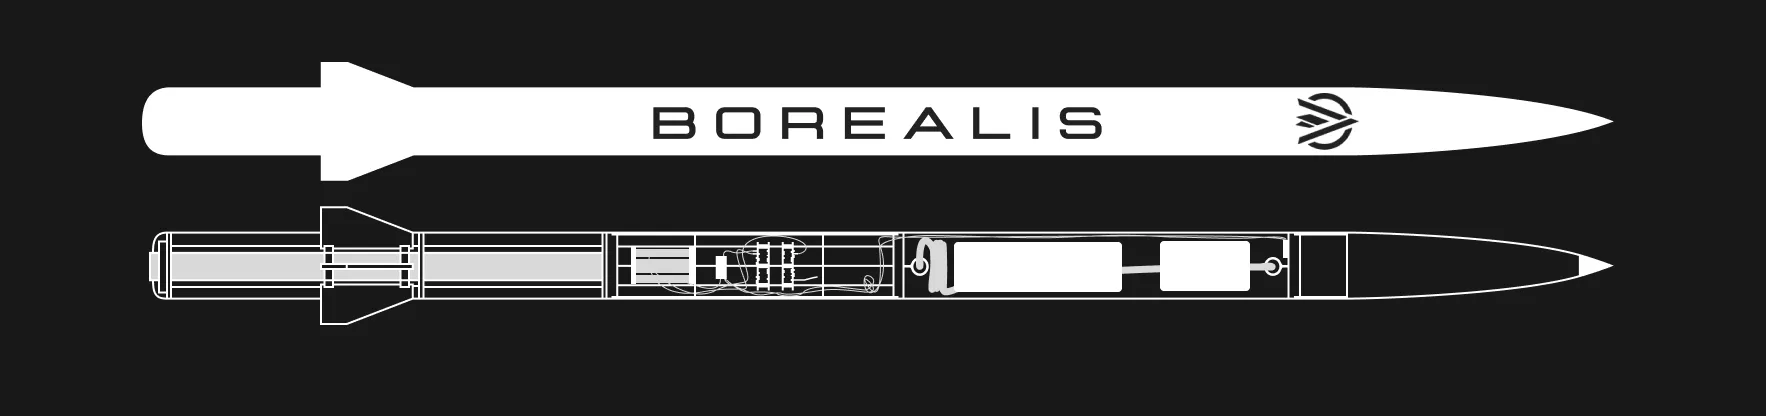
\includegraphics[width=0.75\textwidth]{img/borealis-schema.png}
    \caption{Schema rappresentativo di \emph{Borealis}.}
    % La label ci vuole sempre e te la inventi tu: serve per riferirsi alle immagini successivamente
    \label{fig:borealis-schema}
\end{figure}

Il razzo è formato da una sezione propulsiva (\emph{Motor bay}), una fusoliera
in alluminio divisa in tre \emph{bays}:
\begin{itemize}
    \item \textbf{\emph{Electronics bay}}: contenente l'elettronica di bordo,
    \item \textbf{\emph{Payload bay}}: contenente un carico pagante sperimentale,
    \item \textbf{\emph{Parachute tube}}: contenente i due paracadute.
\end{itemize}
infine un \emph{nose cone} apribile per permettere l'espulsione del paracadute.\\

La \emph{Electronics bay} \'e inserita in una finestra in plexiglass, per permettere
la trasmissione del segnale radio della telemetria, che sarebbe altrimenti schermato
dal corpo in alluminio del razzo. \\

Nella \emph{Electronics bay}
è presente il computer di volo, che si occupa di
gestire il lancio e il recupero del razzo e di raccogliere dati durante il volo. \\
Il computer di volo è dotato di un sistema di telemetria che trasmette in tempo
reale i dati raccolti a una \emph{ground station}, permettendo il monitoraggio
del volo da terra.

\begin{figure}[H]
    \centering
    % Se metti solo una delle due dimensioni, l'altra scala in automatico
    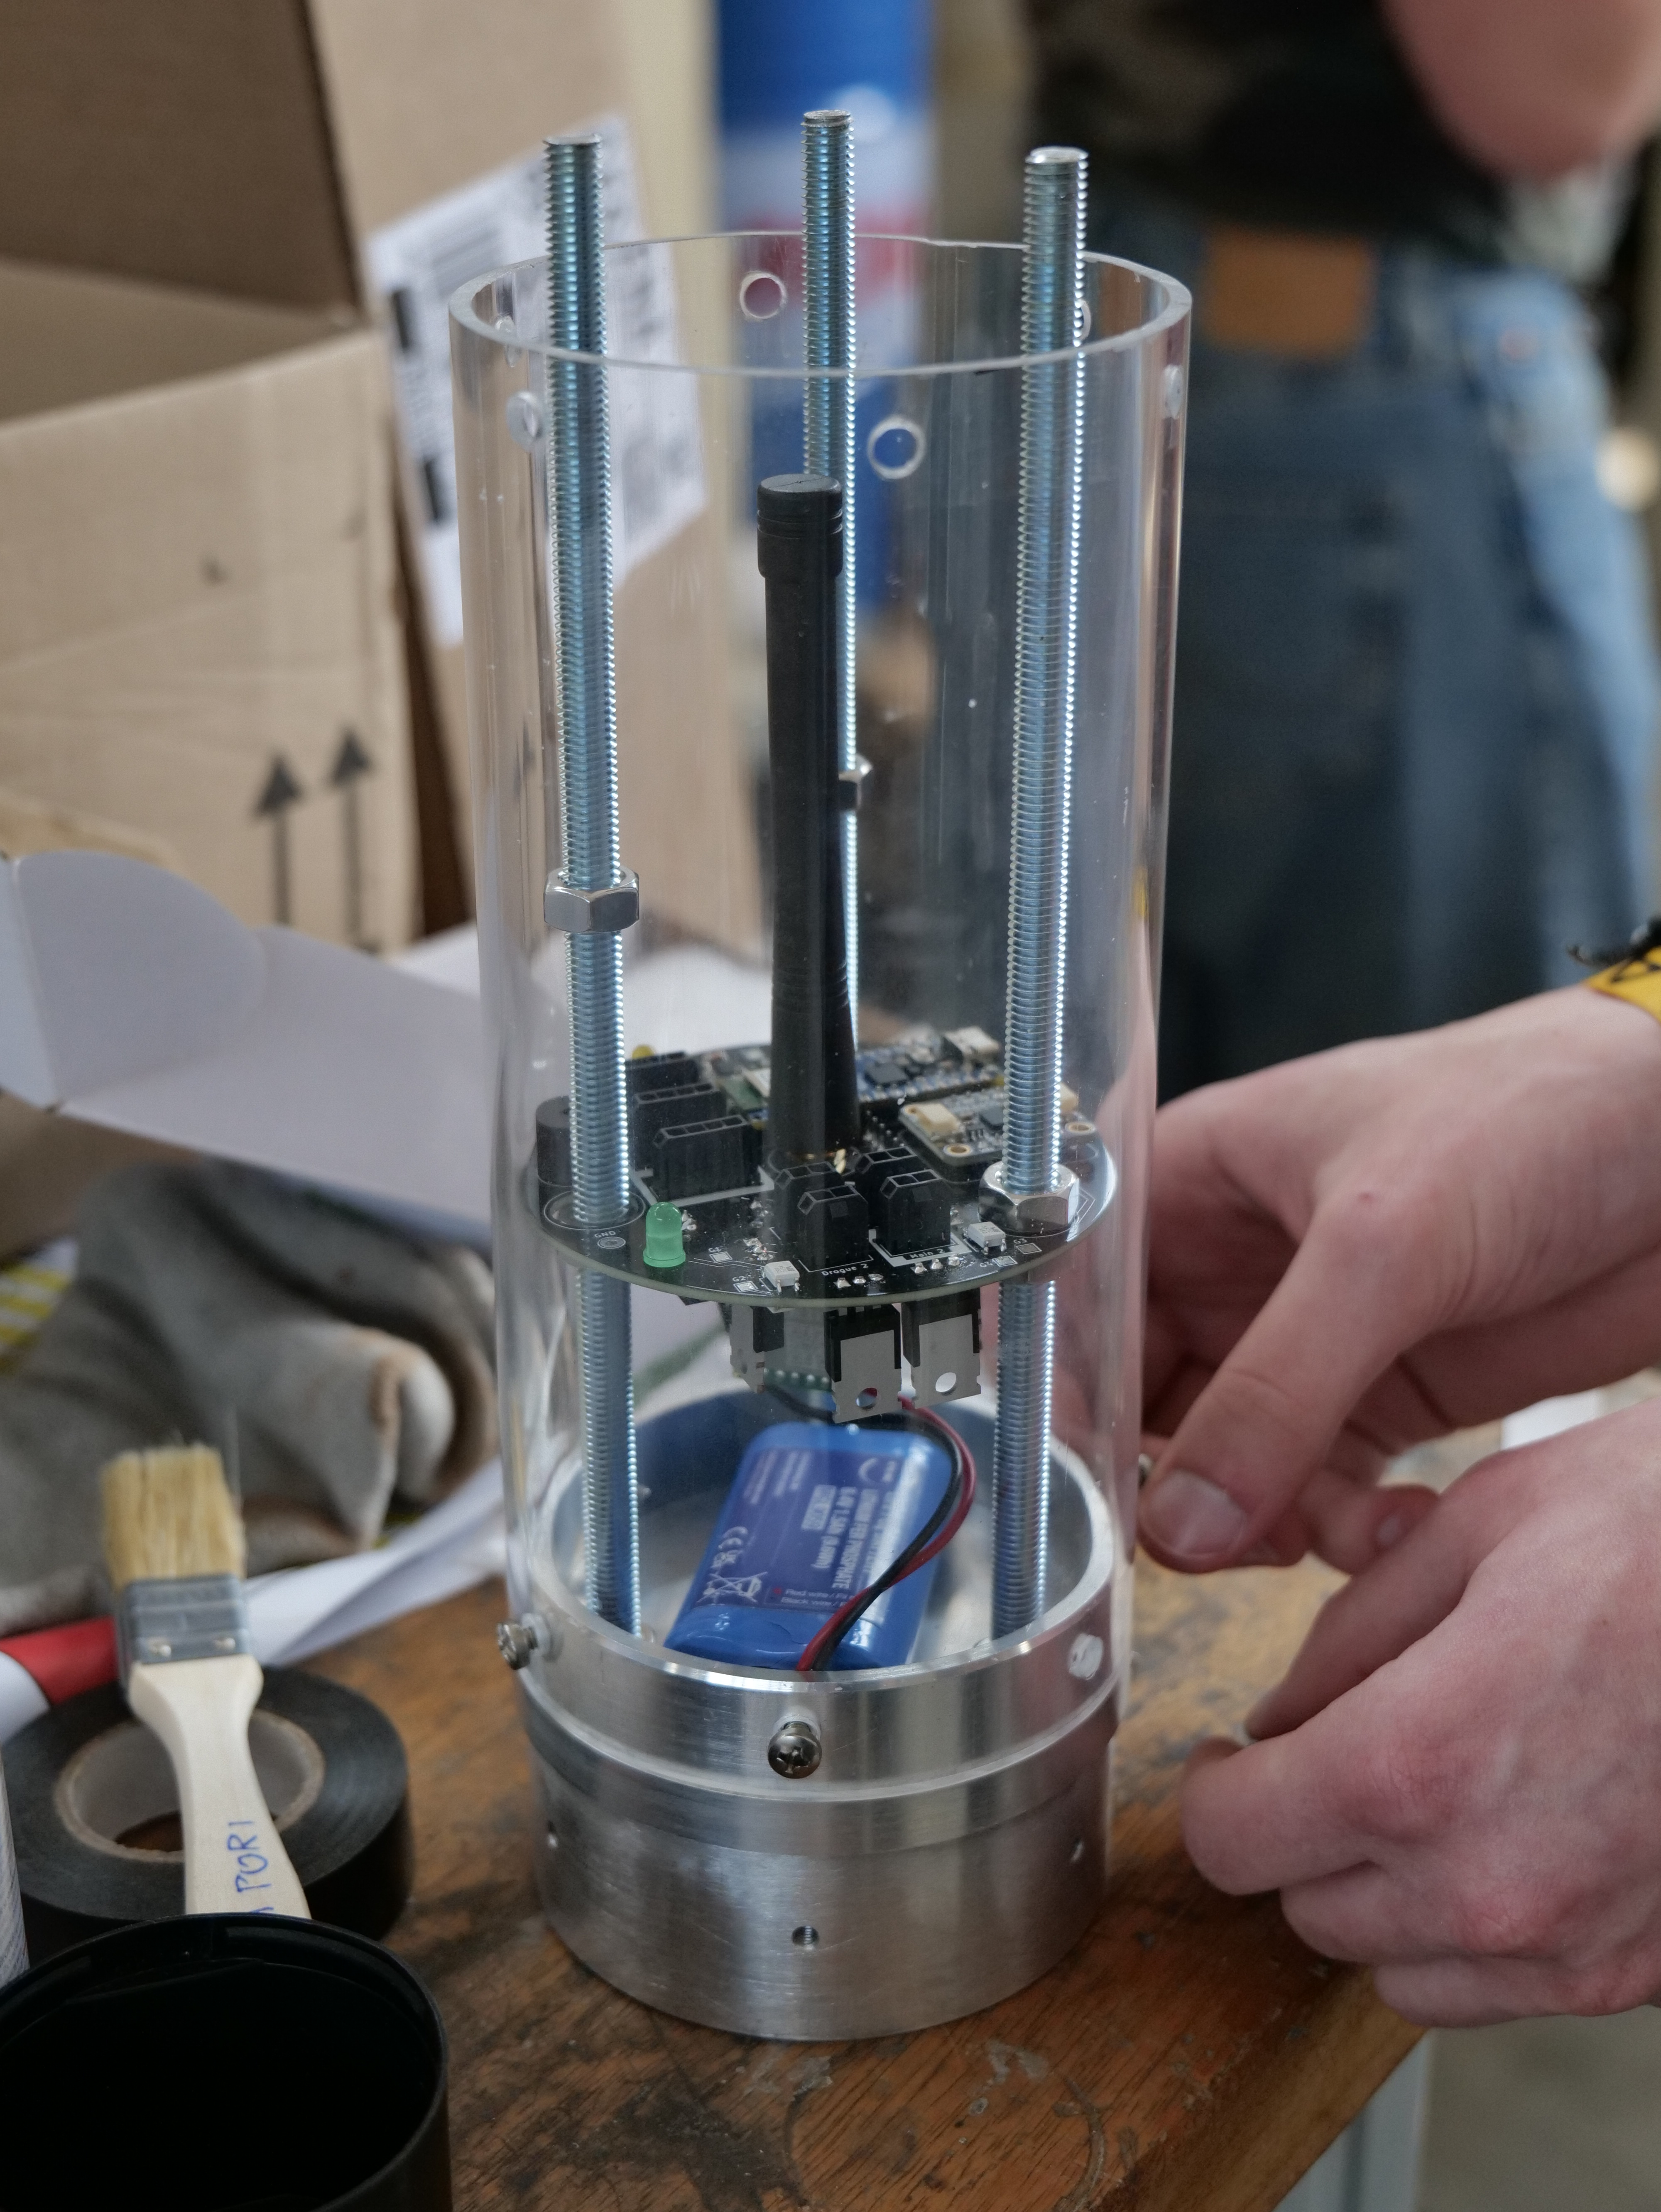
\includegraphics[width=0.6\textwidth]{img/electronics-bay.jpg}
    \caption{\emph{Electronics bay}.}
    % La label ci vuole sempre e te la inventi tu: serve per riferirsi alle immagini successivamente
    \label{fig:electronics-bay}
\end{figure}
\section{Contesto storico della creazione e dell'impiego di razzi sperimentali}
II razzi sperimentali svolgono un ruolo cruciale nella ricerca e nello sviluppo
tecnologico sin dalla fine del XIX secolo.
Sebbene siano stati impiegati per scopi militari sin dal XIII secolo, fu tra il
1926 e il 1929 che il fisico americano Robert H. Goddard, ispirato dagli studi
di Hermann Oberth e Konstantin Tsiolkovsky sulla velocità di fuga terrestre e
sulla propulsione a razzo, realizzò il primo razzo a propellente liquido per
scopi scientifici\cite{seibert2006history}.

Da allora, i razzi sperimentali sono stati utilizzati per una vasta gamma di
applicazioni, tra cui:
\begin{itemize}
    \item La ricerca spaziale e l’esplorazione planetaria, come i razzi-sonda
          impiegati per esperimenti scientifici in microgravità.
    \item Lo studio dell’atmosfera e dei fenomeni meteorologici, come i razzi
          impiegati per analizzare la composizione degli strati superiori
          dell’atmosfera terrestre.
    \item I test di nuove tecnologie aerospaziali, inclusi materiali innovativi,
          sistemi di propulsione sperimentali, sistemi di navigazione autonoma e
          nuove tecnologie di telecomunicazione.
    \item Applicazioni educative e accademiche, che permettono a università e
          centri di ricerca di sviluppare esperimenti e formare studenti nel campo
          dell’ingegneria aerospaziale.
\end{itemize}

\section{Contesto e importanza dei sistemi di telemetria nei razzi sperimentali}
Le motivazioni per cui \`e importante sviluppare un sistema di telemetria per un
razzo sperimentale sono molteplici.

In primo luogo, il monitoraggio del volo in tempo reale permette di avere un
\emph{feedback} immediato sulle prestazioni del razzo, sulle condizioni
ambientali e sulle eventuali anomalie che possono verificarsi durante il volo.
Inoltre, la raccolta di dati durante il volo \`e fondamentale per l’analisi
post missione e per l’ottimizzazione del design del razzo.
Infine, la telemetria \`e essenziale per poter analizzare il volo in caso di
problemi o incidenti, al fine d'identificarne le cause se il sistema di
\emph{logging} a bordo dovesse andare perso.

Ciò pone delle sfide tecniche significative tra cui:
\begin{itemize}
    \item L'affidabilità della trasmissione dati, che deve essere mantenuta
          nonostante le condizioni critiche a cui il sistema è soggetto, tra cui
          accelerazioni estreme, eventi atmosferici e interferenze elettromagnetiche.
    \item L'ottimizzazione della raccolta dati, che deve avvenire in tempo reale
          e con una frequenza sufficiente per garantire la precisione delle misurazioni.
    \item La gestione del consumo energetico, che deve essere minimizzato per
          garantire l'autonomia del sistema durante il volo.
\end{itemize}

\section{Obiettivi della tesi e contributo personale}
L'obiettivo di questa tesi è la descrizione delle fasi di progettazione,
sviluppo e ottimizzazione del sistema di telemetria per il razzo Borealis di
Aurora Rocketry, offrendo una panoramica dettagliata delle tecnologie utilizzate
e delle scelte progettuali effettuate, valutando le prestazioni del sistema e
identificando possibili miglioramenti futuri.
Si vuole inoltre fornire un confronto tra le soluzioni adottate da Aurora
Rocketry e quelle utilizzate in progetti simili, al fine di valutare l'impatto
del sistema sviluppato nell'ambito della ricerca e dello sviluppo di razzi
sperimentali.

Il mio contributo personale al progetto ha riguardato tutte le fasi di sviluppo
del computer di volo, dal design iniziale alla realizzazione del prototipo, fino
alla fase di test e ottimizzazione.
Ho contribuito alla scelta delle tecnologie utilizzate, alla progettazione
dell'architettura del computer di volo e del sistema di telemetria e alla
scrittura del software per la raccolta, la strutturazione e la trasmissione dati.
Inoltre, ho partecipato attivamente alle prove sperimentali e all'analisi dei
dati raccolti, apportando modifiche e ottimizzazioni al sistema in base ai
risultati ottenuti.

\chapter{Descrizione del Computer di Volo} \label{chap:flight-computer}
\pagestyle{plain}

Il computer di volo di Borealis è basato su un microcontrollore ESP32-S3, montato
su una scheda di sviluppo Arduino Nano ESP32, un modulo di raccolta dati contenente
i sensori, e un modulo di attuatori responsabile dell'attivazione di cariche
pirotecniche tramite un circuito di innesco controllato dal microcontrollore.%

I sensori utilizzati sono:
\begin{itemize}
    \item Una \ac{IMU} \emph{Bosch BNO055}\libref{lib:bno055}
          (Giroscopio, Accelerometro e Magnetometro).
    \item Due barometri \emph{Adafruit MPRLS} con presa statica \libref{lib:mprls}.
\end{itemize}
\section{Funzioni principali e componenti chiave}
Il computer di volo si occupa del monitoraggio del volo. Riceve i dati dal modulo
dei sensori, tramite algoritmi di \emph{sensor fusion} li elabora e
contemporaneamente li trasmette alla \emph{ground station}.
In particolare fa uso di un Extended Kalman Filter per filtrare e combinare i
dati ottenuti dalla \ac{IMU} e dei due barometri, ottenendo una stima
affidabile dell'orientamento, della velocità e dell'altitudine.
Il filtro mitiga gli errori dei sensori, corregge la deriva della \ac{IMU} e riduce
le incertezze delle misurazioni barometriche, combinando i dati di accelerazione,
orientamento e pressione atmosferica.

L'algoritmo di rilevamento dell'apogeo monitora l'altitudine e la velocità verticale
del razzo.
Quando la velocità verticale si annulla e il razzo inizia la discesa, il
computer di volo rileva l'apogeo e attiva la sequenza di recupero,
espellendo prima il paracadute \emph{drogue} per stabilizzare il razzo, e poi
il paracadute principale per garantire una discesa controllata.

\section{Integrazione e ruolo del sistema di telemetria}
Per la telemetria è stato impiegato un modulo \ac{LoRa} \emph{EByte E220-900T22D}
a 868MHz collegato al microcontrollore tramite un'interfaccia \ac{UART}
trasmettendo in tempo reale i dati di volo alla ground station.

Il sistema di telemetria è stato integrato nel computer di volo per permettere il
monitoraggio del volo in tempo reale e la raccolta dati durante la missione,
fornendo un'interfaccia di comunicazione tra il razzo e la \emph{ground station}.
Il sistema di telemetria è stato progettato per garantire l'affidabilità della
trasmissione dati, la precisione delle misurazioni e l'ottimizzazione del consumo
energetico.%

Il software di gestione della telemetria è stato sviluppato in C++17 utilizzando
una libreria open-source\libref{lib:lora} per l'interfaccia con il modulo \ac{LoRa}
e un protocollo di comunicazione personalizzato per la trasmissione e la
ricezione dei dati.

\chapter{Tecnologia \texorpdfstring{LoRa\textsuperscript{\textcopyright}}{} e la sua Applicazione} \label{chap:lora}

\section{Panoramica della tecnologia \texorpdfstring{LoRa\textsuperscript{\textcopyright}}{}}
\ac{LoRa} è una tecnologia proprietaria per la trasmissione wireless di dati a
lungo raggio e basso consumo energetico. Impiega la modulazione \ac{CSS},
che garantisce un'elevata robustezza alle interferenze e consente comunicazioni
su lunghe distanze a basso consumo energetico, a costo di una ridotta velocità di trasmissione,
che rimane comunque adeguata per applicazioni di telemetria e monitoraggio
in tempo reale. \\
\ac{LoRa} opera all'interno delle bande di frequenza \ac{ISM} non licenziate,
con specifiche allocazioni in base alla regione geografica:
\begin{itemize}
    \item \textbf{868 MHz} in Europa.
    \item \textbf{915 MHz} in Nord America.
    \item \textbf{433 MHz} in alcune aree dell’Asia.
\end{itemize}

Questa tecnologia può essere utilizzata sia in modalità \emph{point-to-point},
per la comunicazione diretta tra dispositivi, sia in un’architettura di rete più
estesa. In quest'ultimo caso, è comunemente adottata all'interno di
un'infrastruttura \ac{LoRaWAN}, che consente la trasmissione di dati a lunga
distanza tramite una rete di gateway interconnessi a server centralizzati.

\subsection{Modulazione \emph{Chirp Spread Spectrum}}
La modulazione \ac{CSS} è una tecnica di modulazione che fa uso di segnali a
\emph{chirp} per rappresentare informazioni digitali. I \emph{chirp} sono segnali
la cui frequenza varia linearmente nel tempo: quando la frequenza cresce si parla
di \emph{up-chirp}, mentre quando decresce si parla di \emph{down-chirp}.

\begin{figure}[H]
    \centering
    % Se metti solo una delle due dimensioni, l'altra scala in automatico
    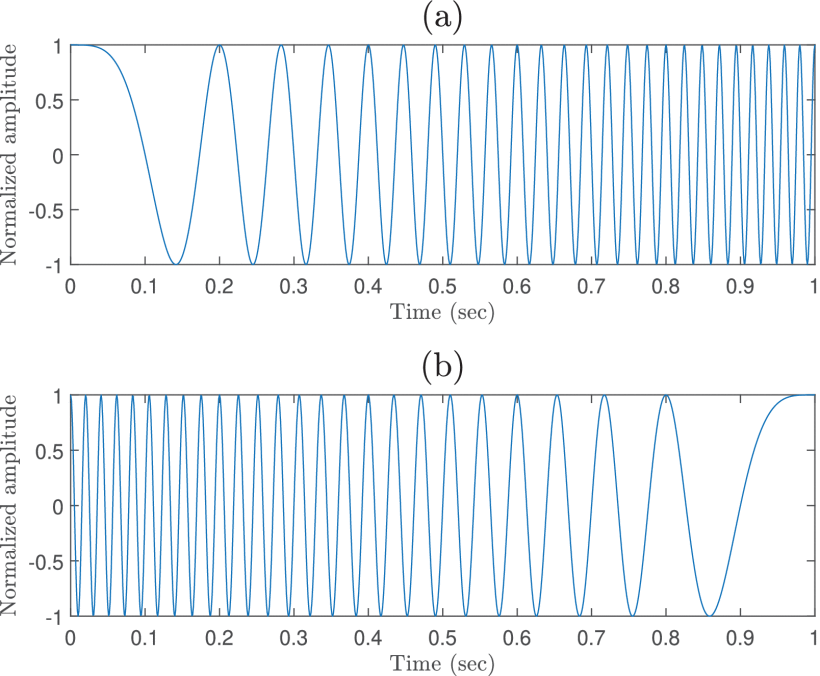
\includegraphics[width=0.75\textwidth]{img/up-chirp-down-chirp.png}
    \caption[Up-chirp e down-chirp]{%
        Esempio temporale di un \emph{up-chirp} (a) e di un \emph{down-chirp} (b).
        \textit{\tiny{Immagine adattata da \cite{10609524}.}}%
    }
    % La label ci vuole sempre e te la inventi tu: serve per riferirsi alle immagini successivamente
    \label{fig:up-chirp-down-chirp}
\end{figure}

In un sistema CSS, ogni simbolo viene rappresentato da un singolo \emph{chirp} e
la quantità di bit che esso trasporta è determinata dallo \ac{SF}, secondo la relazione
$M = 2^{SF}$, dove $M$ rappresenta il numero di simboli ortogonali (cioè distinti
tra loro).

La modulazione \ac{CSS} si basa sulla generazione di un insieme di \emph{chirp}
ortogonali ottenuti mediante traslazioni circolari nel tempo di un \emph{chirp}
di riferimento (detto \emph{chirp base}). La posizione temporale del \emph{chirp}
traslato è proporzionale al valore numerico del simbolo da trasmettere, permettendo
la generazione di $M$ forme d'onda tra loro ortogonali.

Questa proprietà consente al ricevitore di recuperare il simbolo trasmesso mediante
correlazione con i \emph{chirp} possibili, tipicamente implementata in maniera efficiente
tramite la trasformata di Fourier (FFT), rendendo il sistema robusto a rumore,
interferenze e attenuazione multipath\cite{10609524}.

\section{Specifiche tecniche dei moduli utilizzati}

Il sistema di telemetria di Borealis impiega due moduli \ac{LoRa}
\emph{EByte E220-900T22D}, uno in trasmissione a bordo del razzo e uno in
ricezione nella \emph{Ground Station}.
Il modulo impiega la ricetrasmittente \ac{LoRa} \emph{Smart Home LLCC68} e
opera nella banda di frequenza compresa tra 850.15 MHz e 930.15 MHz.

Le specifiche tecniche principali del modulo utilizzato sono riportate nella
Tabella \ref{tab:LoRa-E220-specs}. Queste caratteristiche includono la potenza di
trasmissione massima di +22 dBm (160 mW), la sensibilità del ricevitore pari a
-129 dBm, e la configurabilità dello Spreading Factor (SF) nell'intervallo
SF5 - SF12, che influisce direttamente sulla velocità di trasmissione (da 0.3 kbps
a 62.5 kbps). Inoltre, il consumo energetico del modulo varia tra 120 mA in
trasmissione alla potenza massima e 10 mA in ricezione\dsref{ds:lora}, permettendo una gestione
efficiente delle risorse in missioni di lunga durata.

\begin{table}[H]
    \centering
    \resizebox{\textwidth}{!}{
        \begin{tabular}{|c|c|}
            \hline
            \textbf{Caratteristica}                      & \textbf{Valore}         \\ \hline
            \textbf{Banda di frequenza}                  & 850.15 MHz - 930.15 MHz \\ \hline
            \textbf{Potenza di trasmissione}             & +22 dBm (160 mW)        \\ \hline
            \textbf{Sensibilità del ricevitore}          & -129 dBm                \\ \hline
            \textbf{Spreading Factor (SF)}               & SF5 - SF12              \\ \hline
            \textbf{Velocità di trasmissione}            & 0.3 kbps - 62.5 kbps    \\ \hline
            \textbf{Consumo in trasmissione (a +22 dBm)} & 120 mA                  \\ \hline
            \textbf{Consumo in ricezione}                & 10 mA                   \\ \hline
            \textbf{Interfaccia di comunicazione}        & \ac{UART} (3.3V TTL)    \\ \hline
            \textbf{Baud rate}                           & 1200 bps - 115200 bps   \\ \hline
            \textbf{Connettore antenna}                  & SMA femmina             \\ \hline
            \textbf{Impedanza connettore}                & 50 \textohm             \\ \hline
        \end{tabular}
    }
    \caption{Caratteristiche tecniche del modulo \ac{LoRa} EByte E220-900T22D.}
    \label{tab:LoRa-E220-specs}
\end{table}

\section{Specifiche delle antenne utilizzate} \label{sec:antennas}
La scelta delle antenne per il sistema telemetrico del razzo è stata guidata da
esigenze tecniche specifiche, nonostante le opzioni disponibili fossero limitate.
Le caratteristiche fondamentali del sistema richiedevano un'antenna a bordo in
grado di garantire una copertura di radiazione uniforme su una superficie quanto
più ampia possibile. Per la \emph{ground station}, invece, è stata selezionata
un'antenna direzionale.

\subsection*{Antenna omnidirezionale (Razzo)}

Per il razzo, la soluzione ottimale si è rivelata essere un'antenna omnidirezionale
elicoidale.
Questa scelta è praticamente obbligata a causa della variazione costante dell'orientamento
del razzo durante il volo, rendendo impraticabile l'utilizzo di antenne direzionali,
a meno di non implementare sistemi complessi di controllo dell'assetto, che
tuttavia non rientrano nell'ambito del progetto attuale.

\subsection*{Antenna direzionale (Ground Station)}

Per la \emph{ground station}, è stata selezionata un'antenna direzionale. Le due
tecnologie principali prese in considerazione sono state:
\begin{itemize}
    \item Antenna Yagi
    \item Antenna Log-Periodica
\end{itemize}

La differenza principale tra questi due tipi di antenne riguarda la direzionalità.
L'antenna Log-Periodica offre una direzionalità maggiore rispetto alla Yagi,
caratteristica che, in linea di principio, sarebbe desiderabile per il sistema
di terra, in quanto consente di concentrare l'energia di ricezione in un angolo
ristretto, aumentando il guadagno e riducendo il rumore di fondo.
Tuttavia, l'eccessiva direzionalità della Log-Periodica avrebbe introdotto
delle complicazioni operative. Poiché il tracciamento del razzo durante il volo
sarà eseguito manualmente, una direzionalità troppo elevata avrebbe richiesto
una precisione di puntamento molto elevata, difficile da mantenere senza
strumenti automatizzati, aumentando il rischio di perdita temporanea del segnale.

L'antenna Yagi, con la sua direzionalità moderata, si è rivelata una scelta più
equilibrata. Essa offre un buon compromesso tra guadagno e facilità di puntamento,
consentendo un tracciamento sufficientemente preciso del razzo senza la necessità
di strumenti avanzati d'inseguimento automatico.

\subsection*{Dettagli tecnici delle antenne}

\begin{table}[H]
    \centering
    \resizebox{\textwidth}{!}{
        \begin{tabular}{|c|c|c|}
            \hline
                                & \textbf{Antenna Omnidirezionale} & \textbf{Antenna Yagi}   \\ \hline
            Marca e modello     & \emph{Siretta Delta 5A}          & \emph{Siretta Oscar 3A} \\ \hline
            Tipo                & Omnidirezionale elicoidale       & Direzionale Yagi        \\ \hline
            Frequenza di lavoro & 433 MHz - 5.9 GHz                & 850 MHz - 930 MHz       \\ \hline
            Guadagno            & 3 dBi                            & 10.55 dBi               \\ \hline
            Angolo di copertura & 360\textdegree                   & 60\textdegree           \\ \hline
            Impedenza           & 50 \textohm                      & 50 \textohm             \\ \hline
            Polarizzazione      & Verticale                        & Verticale               \\ \hline
            Tipo di connettore  & SMA maschio                      & FME maschio             \\ \hline
        \end{tabular}
    }
    \caption{Specifiche tecniche dell'antenna omnidirezionale e dell'antenna Yagi.}
    \label{tab:antenne_confronto}
\end{table}

\begin{figure}[H]
    \centering
    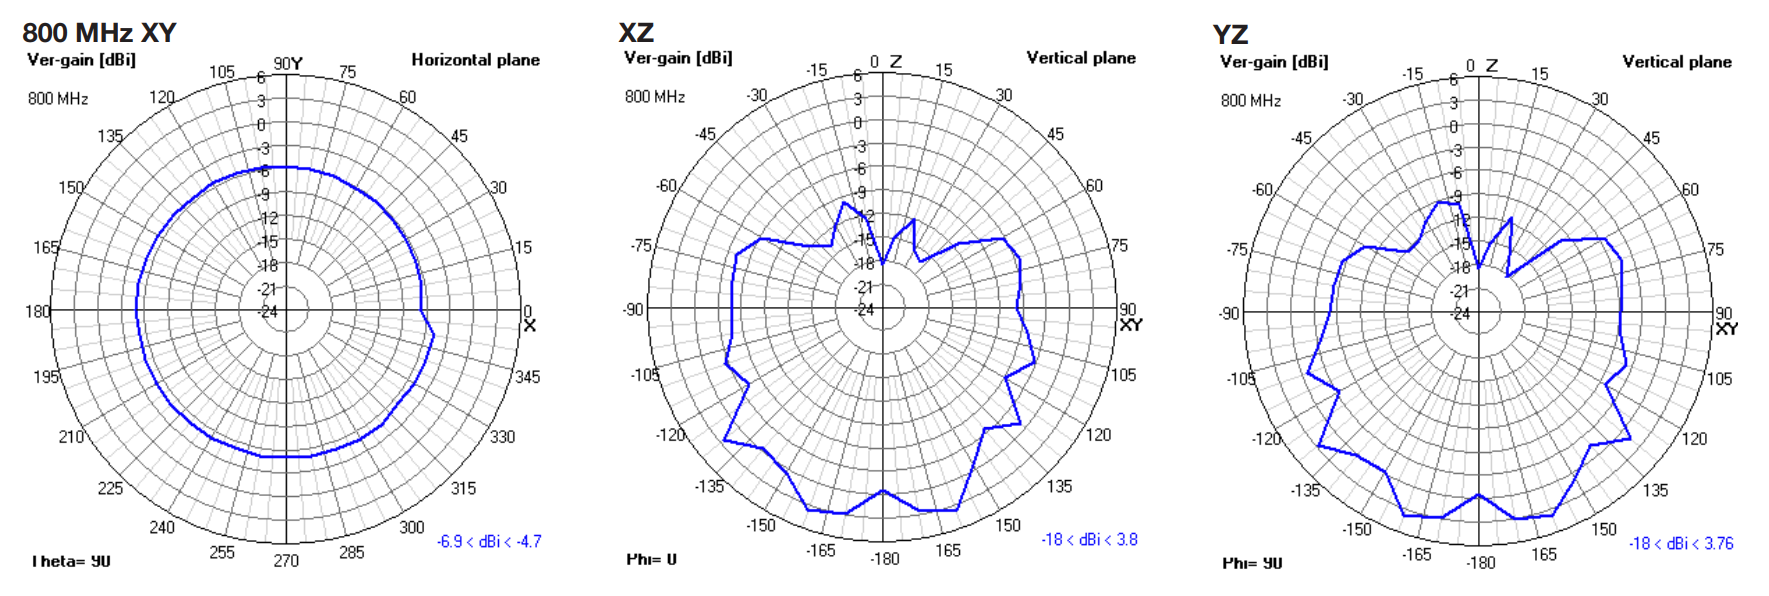
\includegraphics[width=\textwidth]{img/omnidirezionale-rad-plot.png}
    \caption[Grafici di radiazione antenna omnidirezionale]%
    {Grafici di radiazione dell'antenna omnidirezionale. \tiny{Immagine adattata da \dsref{ds:omni}}}%
    \label{fig:omni-rad-plot}
\end{figure}

\begin{figure}[H]
    \centering
    % Se metti solo una delle due dimensioni, l'altra scala in automatico
    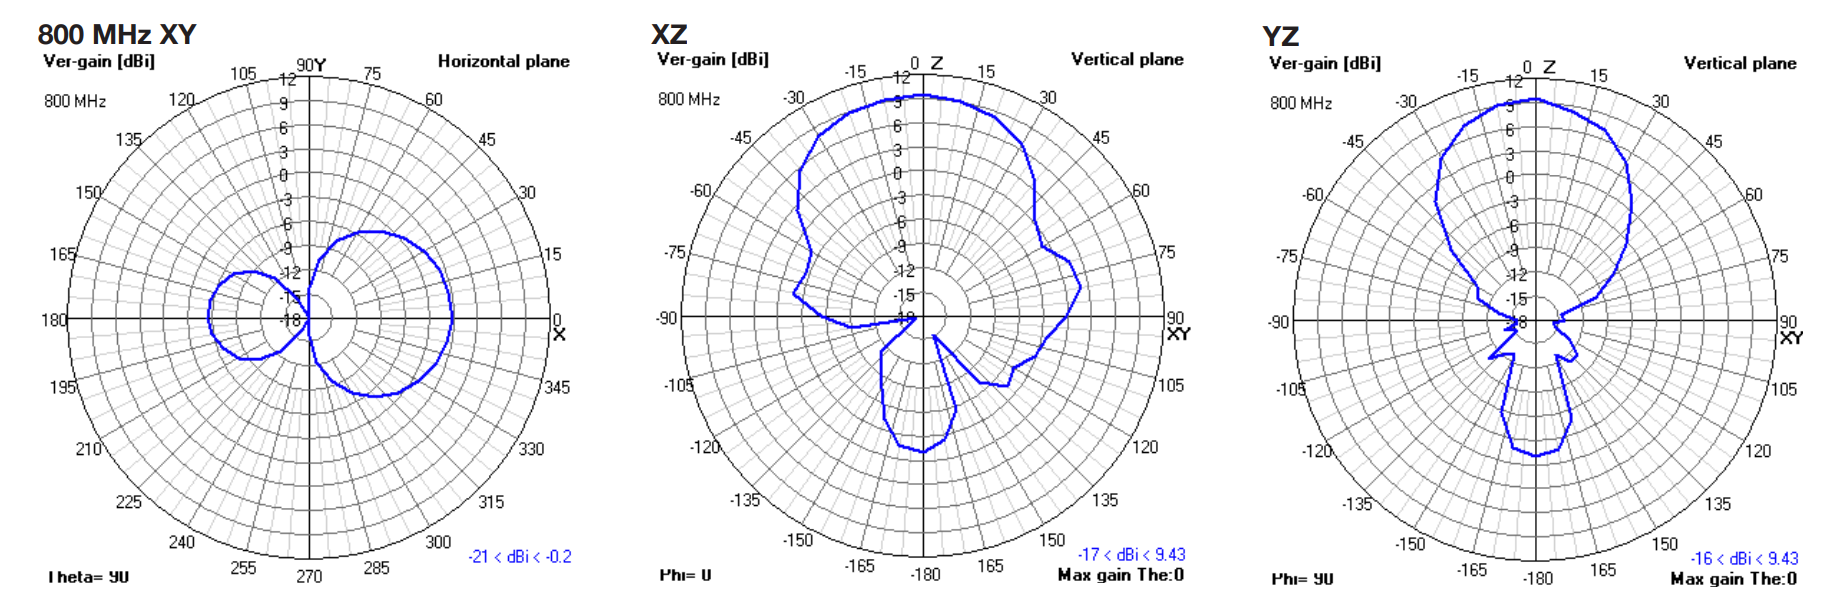
\includegraphics[width=\textwidth]{img/yagi-rad-plot.png}
    \caption[Grafici di radiazione dell'antenna Yagi]%
    {Grafici di radiazione dell'antenna Yagi. \tiny{Immagine adattata da \dsref{ds:yagi}}}%
    % La label ci vuole sempre e te la inventi tu: serve per riferirsi alle immagini successivamente
    \label{fig:yagi-rad-plot}
\end{figure}

\section{Motivazioni della scelta di \texorpdfstring{LoRa\textsuperscript{\textcopyright}}{} per il progetto}
Il progetto richiedeva di individuare una tecnologia di trasmissione dati che garantisse
un'elevata affidabilità e copertura, mantenendo un consumo energetico contenuto,
anche in un ambiente operativo complesso come quello di un razzo sperimentale.

Le caratteristiche tecniche discusse nelle sezioni precedenti rendono \ac{LoRa}
una scelta ideale per il progetto.
I test effettuati in laboratorio hanno confermato la capacità dei moduli
ricetrasmittenti impiegati di soddisfare i requisiti di trasmissione dati del
sistema di telemetria.

In letteratura sono stati documentati numerosi casi di applicazione di \ac{LoRa}
in sistemi simili\cite{Misbahuddin2022, Ma2024}, che hanno dimostrato la sua
efficacia in ambienti operativi critici, garantendo trasmissioni dati stabili e
affidabili.

Infine, l'ampia diffusione dell'uso di \ac{LoRa} nell'\ac{IoT} e la conseguente
vasta disponibilità di hardware a costi contenuti hanno reso questa tecnologia
una scelta conveniente e accessibile per il progetto.

\chapter{Implementazione del Sistema di Telemetria} \label{chap:telemetry}

% In questo capitolo verranno discussi i dettagli di progettazione e di implementazione
% del software che gestisce la telemetria a bordo di Borealis e nella \emph{ground station}.

\section{Architettura del sistema di trasmissione dati}
Il sistema di trasmissione dati impiegato su Borealis è basato su un'architettura
punto-punto monodirezionale.

Come discusso nel capitolo \ref{chap:lora} il sistema è composto dai seguenti componenti principali:
\begin{itemize}
    \item \textbf{Modulo \ac{LoRa} trasmettitore (Razzo)}: EByte E220-900T22D per
          la trasmissione della telemetria alla \emph{ground station} con antenna
          omnidirezionale (Sez. \ref{sec:antennas}).
          Collegato tramite interfaccia \ac{UART} al computer di volo.
    \item \textbf{Modulo \ac{LoRa} ricevitore (Ground Station)}: EByte E220-900T22D,
          identico al ricevente, impiegato nella \emph{ground station} per
          ricevere i dati con antenna direzionale Yagi (Sez. \ref{sec:antennas}).
          Collegato a un microcontrollore ESP32-S3 tramite interfaccia \ac{UART}
          che si occupa di inviare i dati ricevuti a un PC tramite connessione seriale.
\end{itemize}

Il flusso dei dati nel sistema è il seguente:

% \begin{figure}[H]
%     \centering
%     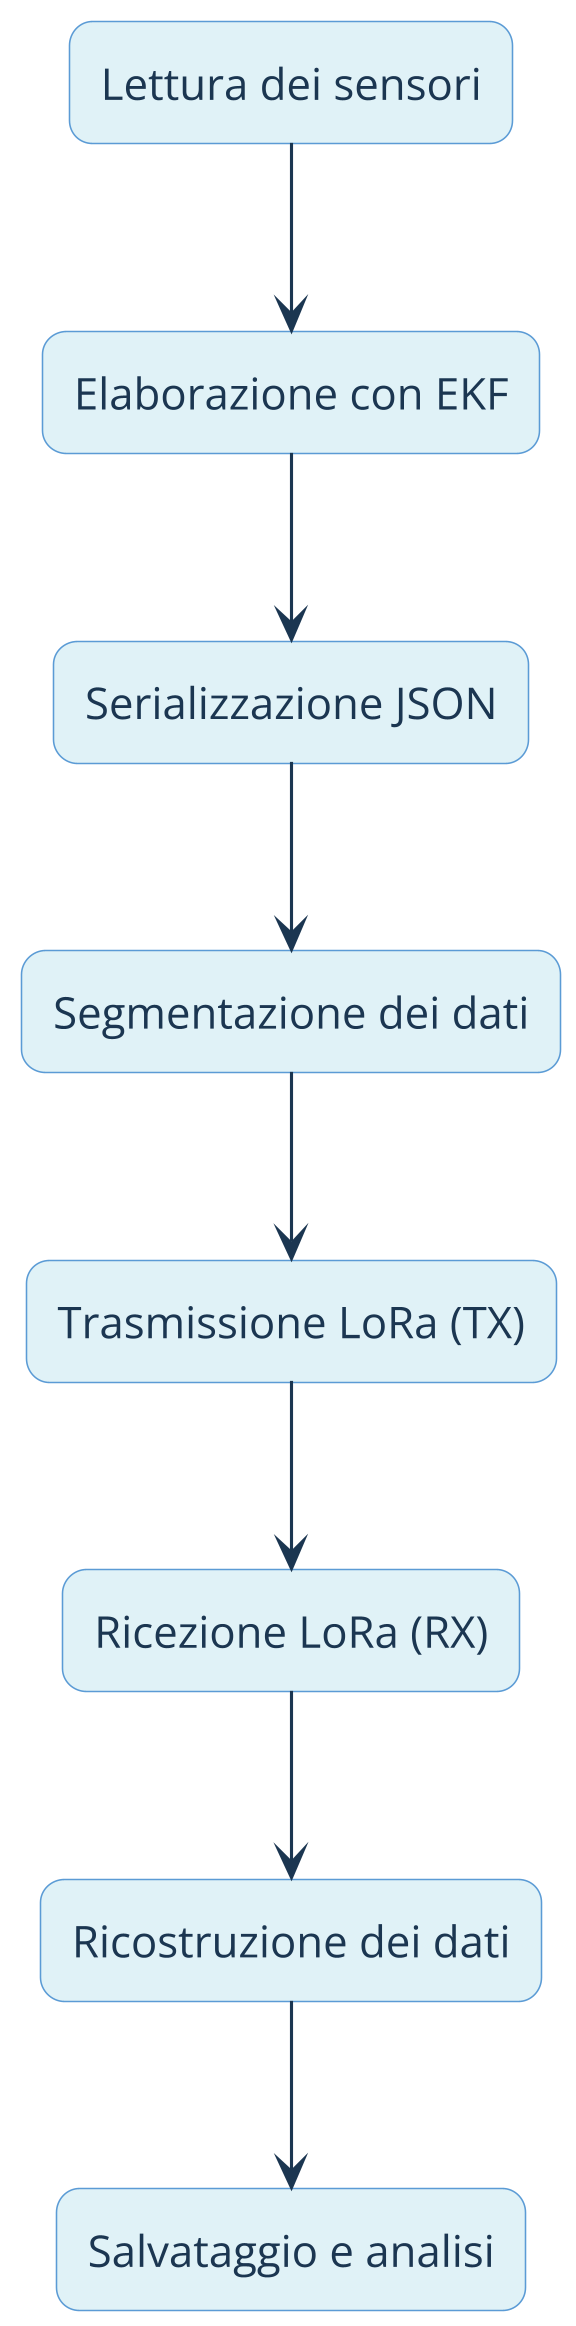
\includegraphics[width=0.25\textwidth]{img/uml/data-flow.png}
%     \caption{Schema di flusso dei dati del sistema di telemetria.}
%     \label{fig:telemetry-flowchart}
% \end{figure}
% \newpage
\begin{enumerate}
    \item I dati di volo vengono raccolti dai sensori a bordo del razzo e inviati al computer di volo.
    \item Il computer di volo elabora i dati attraverso un \ac{EKF} che permette di derivare l'altitudine e la velocità verticale del razzo.
    \item I dati elaborati vengono inseriti in un oggetto JSON.
    \item L'oggetto JSON viene serializzato e segmentato per rispettare i limiti di dimensione del payload dei moduli \ac{LoRa}.
    \item Ogni segmento viene inserito in un pacchetto ad-hoc per gestire la logica di trasmissione e ricezione.
    \item I dati serializzati vengono trasmessi al modulo \ac{LoRa} trasmettitore via \ac{UART}
    \item Il modulo \ac{LoRa} trasmettitore invia i pacchetti dati via wireless.
    \item Il modulo \ac{LoRa} ricevitore riceve i dati trasmessi.
    \item I dati ricevuti vengono deserializzati, ricomponendo il \emph{payload} originale.
    \item Il \emph{payload} viene inviato al PC per essere salvati e in seguito analizzati.
\end{enumerate}
Vista la presenza di forti vibrazioni, accelerazioni estreme,
variazioni continue di assetto e orientamento, condizioni atmosferiche variabili
e possibili interferenze elettromagnetiche, sono stati valutati
gli impatti che questi fattori possono avere sulla trasmissione dei dati e sulla
loro integrità. \\
Abbiamo calcolato che la banda di frequenza di 868 MHz, utilizzata dai moduli
\ac{LoRa} impiegati, non è soggetta a interferenze significative da parte di altri
dispositivi e che la modulazione \ac{CSS} impiegata garantisce una robustezza
adeguata contro le interferenze, il rumore ambientale e l'effetto Doppler,
permettendo una trasmissione affidabile anche in condizioni difficili.
Bisogna inoltre tenere conto che nella \emph{ground station} non \'e previsto
alcun sistema di inseguimento, quindi l'antenna direzionale Yagi deve essere puntata manualmente
verso il razzo durante il volo, per garantire una ricezione ottimale del segnale.

\section{Protocollo di comunicazione e gestione dati}

Il protocollo di comunicazione è stato progettato per garantire efficienza e
semplicità, consentendo la trasmissione di pacchetti dati strutturati e adattabili
a diversi formati.

Il pacchetto generato dal nodo trasmittente è composto dalle seguenti sezioni:

\begin{itemize}
    \item \textbf{\emph{Header} fisico} (3 byte), che include:
          \begin{itemize}
              \item Byte alto dell’indirizzo del destinatario
              \item Byte basso dell’indirizzo del destinatario
              \item Identificativo del canale di trasmissione
          \end{itemize}
    \item \textbf{\emph{Payload}} (196 o 197 byte): contiene i dati applicativi da trasmettere.

    \item \textbf{\emph{Footer} opzionale} (1 byte): include il valore del \ac{RSSI},
          utilizzato per la diagnostica della qualità del link.
\end{itemize}

Considerando le limitazioni fisiche del modulo \ac{LoRa} impiegato (in particolare,
la dimensione massima dei pacchetti), il protocollo è stato esteso per supportare
la segmentazione del \emph{payload}. Quando il dato da trasmettere eccede la dimensione
massima consentita, esso viene suddiviso in sotto-segmenti detti \emph{chunk},
ciascuno trasmesso come pacchetto indipendente.

Per supportare questa funzionalità è stato introdotto un \textbf{header logico}
aggiuntivo di 11 byte in testa al \emph{payload}, che include le seguenti informazioni di controllo:

\begin{itemize}
    \item \textbf{\emph{Packet Number}}: identificatore univoco della sequenza di pacchetti riferita a una singola lettura.
    \item \textbf{\emph{Total Chunks}}: numero totale di chunk in cui è stato suddiviso il \emph{payload} originale.
    \item \textbf{\emph{Chunk Index}}: indice progressivo del chunk corrente all'interno della sequenza, utilizzato per la ricostruzione corretta del dato.
    \item \textbf{\emph{Payload Size}}: dimensione effettiva del \emph{payload} trasportato nel chunk, espressa in byte.
    \item \textbf{\emph{Timestamp}}: riferimento temporale associato all’invio del pacchetto, utile per analisi temporali e sincronizzazione.
    \item \textbf{\emph{Protocol Version}}: campo riservato per la gestione di versioni successive del protocollo, utile in ottica di retrocompatibilità.
\end{itemize}

Considerando la dimensione del \emph{header} logico, il \emph{payload} massimo trasportabile in un singolo pacchetto
è di 185 byte usando i moduli \ac{LoRa} EByte E220-900T22D, che hanno un limite di 200 byte per pacchetto.

\section{Implementazione software e algoritmi di gestione della trasmissione}
Il software è stato implementato in C++17. Nei seguenti paragrafi verrà illustrata
l'architettura dei principali moduli software: il computer di volo,
il modulo trasmettitore e il modulo ricevitore.

\subsection{Architettura software}

\subsubsection{Computer di volo}
Il computer di volo è responsabile della raccolta e dell'elaborazione dei dati
provenienti dai sensori, della gestione della telemetria e dell'attivazione degli
attuatori per il recupero del razzo.

Il sistema è orchestrato da una macchina a stati finiti, che gestisce le diverse
fasi del volo, rappresentata nella Figura \ref{fig:flight-computer-fsm}.
\ifdefined\HCode
\else
    \begin{landscape}
        \fi
        \begin{figure}[H]
            \centering
            \vspace*{2cm}  % Reduce space from top
            \hspace*{-4cm}
            
\includegraphics[width=1.7\textwidth]{img/uml/fsm.png}
            \caption{Macchina a stati finiti del computer di volo.}
            \label{fig:flight-computer-fsm}
            \vspace*{-1cm}  % Reduce space at bottom
        \end{figure}
        \thispagestyle{empty}  % Remove page numbering for this page
        \ifdefined\HCode
        \else
    \end{landscape}
\fi

\newpage
Il computer di volo è composto da 4 elementi principali:
\paragraph{\textbf{Modulo di raccolta dati:}} Gestisce la lettura dei sensori.
\begin{figure}[H]
    \centering
    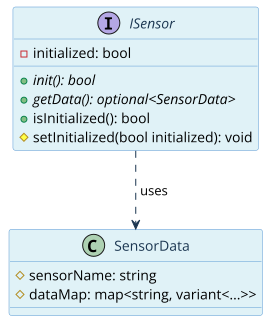
\includegraphics[width=0.5\textwidth]{img/uml/sensor.png}
    \caption{Interfaccia per la raccolta dati da un sensore.}
    \label{fig:flight-computer-data-collection}
\end{figure}

\newpage
\paragraph{\textbf{Modulo di logging:}}Si occupa della serializzazione dei dati in formato JSON.
\begin{figure}[H]
    \centering
    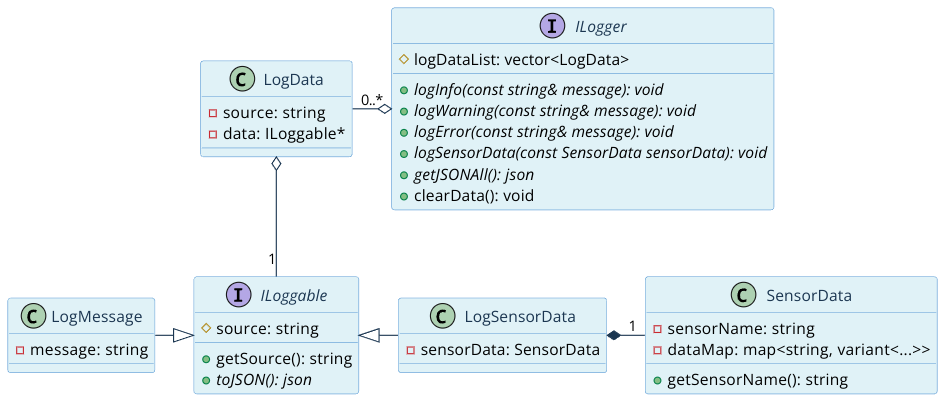
\includegraphics[width=1\textwidth]{img/uml/logger.png}
    \caption{Interfaccia per il logging dei dati.}
    \label{fig:flight-computer-logger}
\end{figure}

\newpage
\paragraph{\textbf{Modulo di elaborazione dati:}}Si occupa dell'elaborazione dei
dati raccolti dai sensori, applicando un \ac{EKF} e algoritmi di \emph{sensor
    fusion} per la stime dell'altitudine e della velocità verticale, che sono
utilizzate per il rilevamento dell'apogeo e la gestione della sequenza di recupero.

\newpage
\paragraph{\textbf{Modulo di telemetria:}}Si occupa della serializzazione, segmentazione
e trasmissione dei dati via \ac{LoRa}.
\begin{figure}[H]
    \centering
    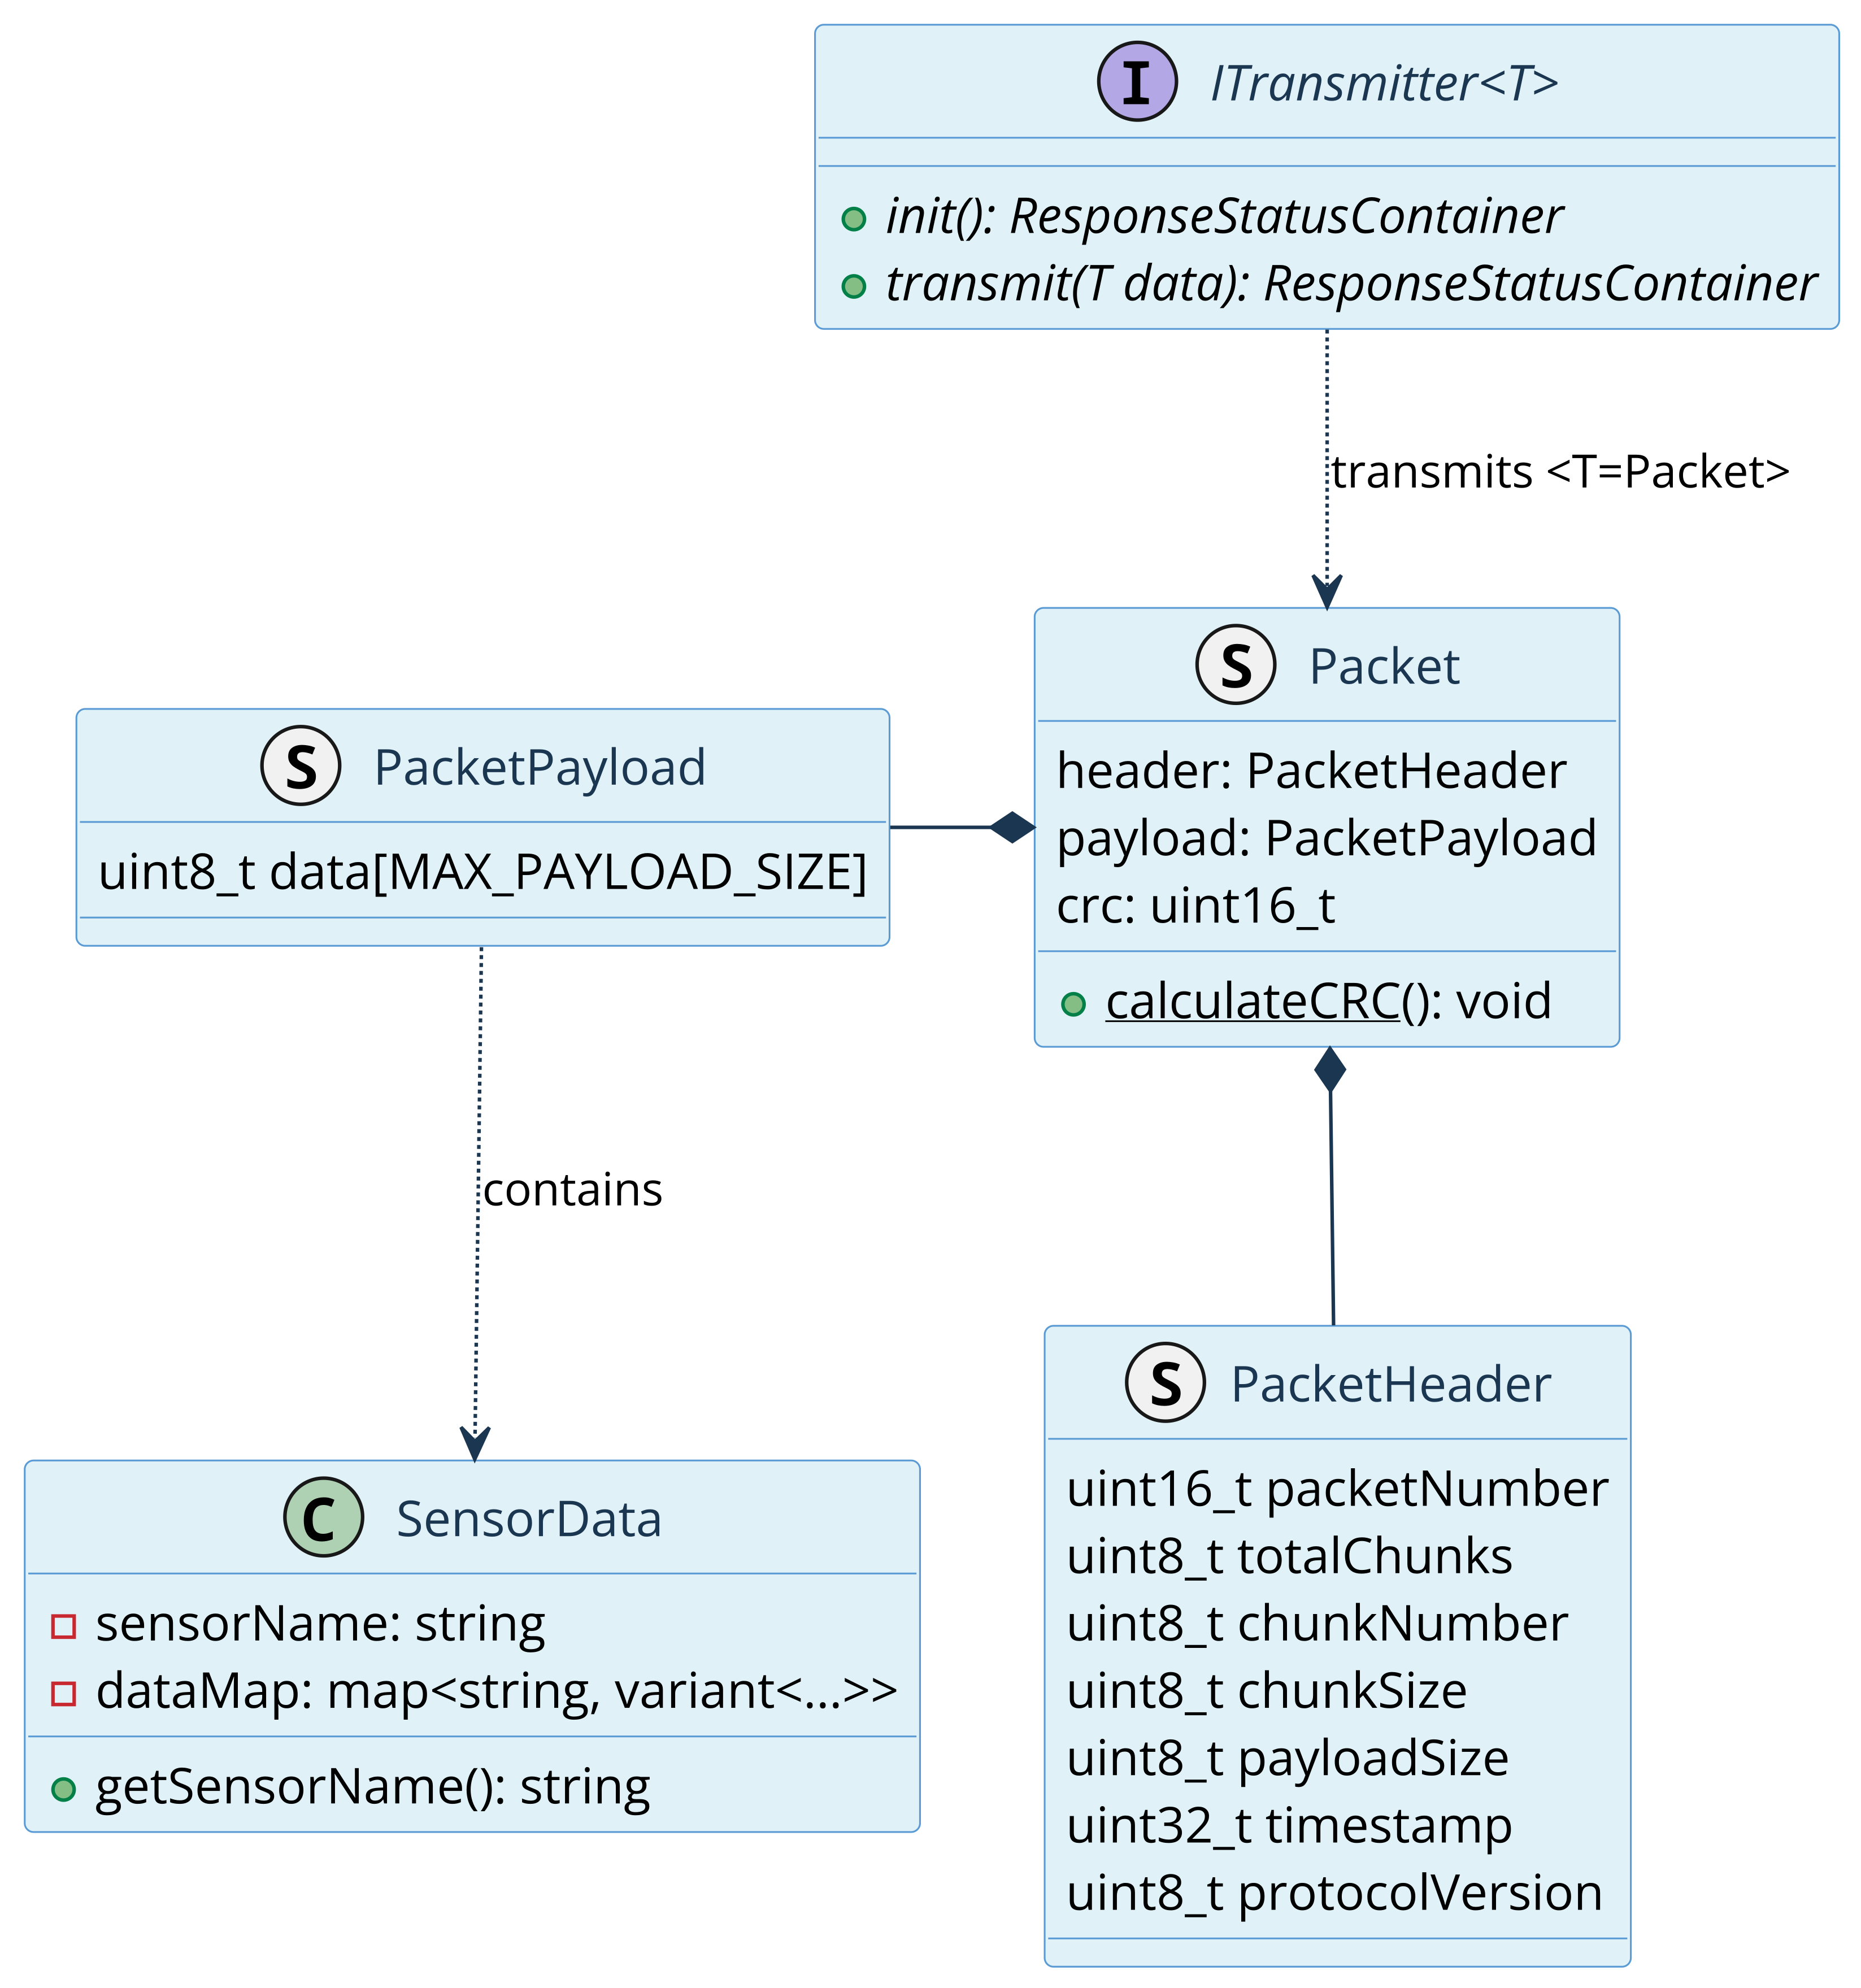
\includegraphics[width=0.8\textwidth]{img/uml/transmitter.png}
    \caption{Interfaccia per la telemetria.}
    \label{fig:flight-computer-telemetry}
\end{figure}
\newpage
\subsubsection{Ground Station}
La \emph{ground station} è responsabile della ricezione dei dati trasmessi dal
razzo, della loro deserializzazione e dell'invio al PC su cui vengono salvati.
\begin{figure}[H]
    \centering
    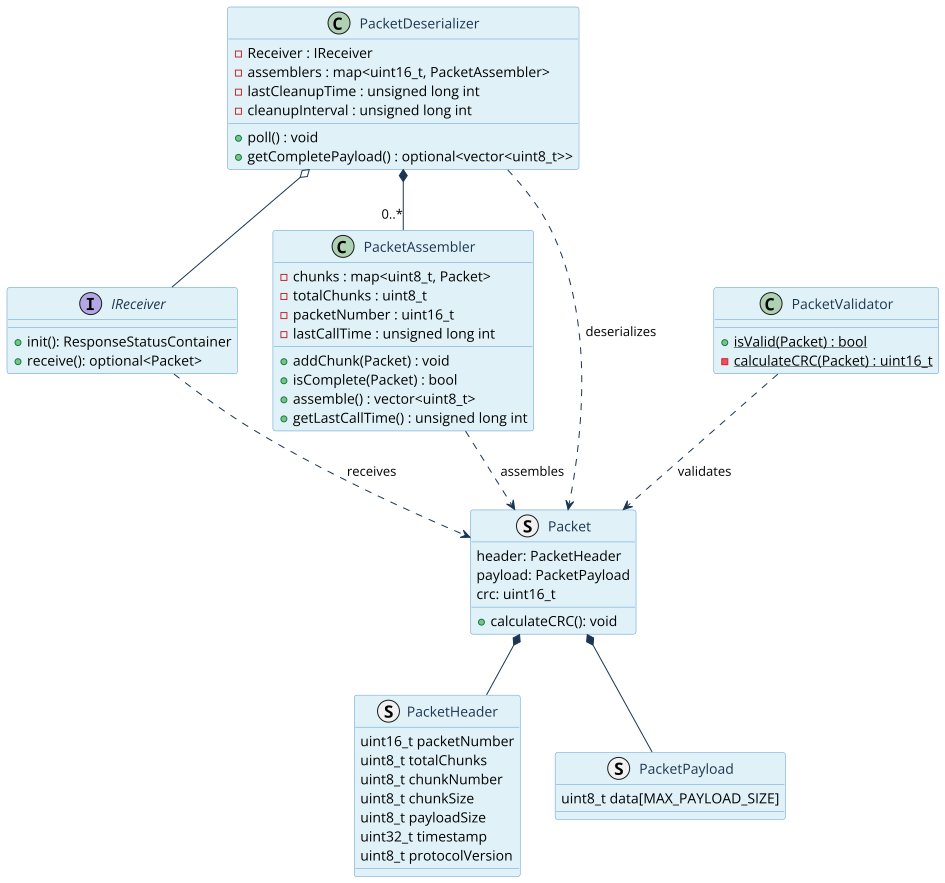
\includegraphics[width=\textwidth]{img/uml/ground-station.png}
    \caption{Architettura della \emph{ground station}.}
    \label{fig:ground-station-architecture}
\end{figure}
\newpage
\subsection{Algoritmo di ricostruzione del \emph{payload}} \label{sec:reconstruction-algorithm}
L'algoritmo di ricostruzione del \emph{payload} originale a partire dai pacchetti
ricevuti, permette di gestire la segmentazione dei dati e garantire l'integrità
delle informazioni trasmesse.

L'algoritmo organizza i pacchetti ricevuti in base al loro identificativo di sequenza
(\emph{Packet Number}), consentendo la ricostruzione dei messaggi frammentati.
Ogni pacchetto in arrivo viene validato, verificando la consistenza dell'\emph{header} logico
e il \ac{CRC} per assicurare l'integrit\'a del contenuto.

I pacchetti validati vengono inseriti in una struttura dati temporanea, corrispondente
alla sequenza a cui appartengono, indicizzandoli in base al \emph{Chunk Number}.
Una volta ricevuti tutti i \emph{chunk} previsti per una sequenza, il \emph{payload}
originale viene ricostruito, concatenando i dati dei \emph{chunk}.

Per ottimizzare l'uso delle risorse, \'e stato implementato un meccanismo di \emph{drop}
temporizzato per le sequenze incomplete, prevenendo cos\'i l'accumulo di dati parziali,
sfruttando la tolleranza del sistema alla perdita occasionale di letture dei dati
dei sensori e la garanzia di disponibilità dei dati grazie al sistema di logging secondario a
bordo del computer di volo.

\chapter{Valutazione delle Prestazioni} \label{chap:performance}
\vspace{-0.5cm}
\section{Metodologia di test e criteri di valutazione}
\begin{table}[H]
    \centering
    \renewcommand{\arraystretch}{1.2}
    \begin{tabular}{|p{4cm}|p{6.5cm}|p{4cm}|}
        \hline
        \textbf{Test}                     & \textbf{Obiettivo}                                                                                                                                                                       & \textbf{Metrica misurata}                                     \\
        \hline
        Affidabilit\'a della trasmissione & Verificare la capacit\'a del sistema di trasmettere e ricevere pacchetti su distanze variabili, in condizioni ambientali diverse, con ostacoli, rumore e disallineamento tra le antenne. & \ac{RSSI}, angolo di disallineamento tra le antenne           \\
        \hline
        Throughput                        & Valutare la velocità effettiva di trasmissione su diversi scenari di distanza e ambiente                                                                                                 & Pacchetti/s, bit/s, percentuale di pacchetti persi, \ac{RSSI} \\
        \hline
        Segmentazione e ricostruzione     & Verificare l'efficienza e la scalabilità del protocollo nel ricostruire correttamente i payload segmentati                                                                               & Tempo medio di ricostruzione                                  \\
        \hline
        Meccanismo di \emph{drop}         & Verificare la capacità del sistema di identificare e scartare pacchetti incompleti o corrotti                                                                                            & Loss rate (\%), pacchetti scartati,                           \\
        \hline
        Riordinamento dei \emph{chunk}    & Verificare la capacità del sistema di gestire chunk ricevuti in ordine scorretto e ripristinare l'ordine corretto prima della ricostruzione                                              & Stato di ordinamento                                          \\
        \hline
        Robustezza e affidabilità         & Valutare la stabilità del sistema durante trasmissioni prolungate e in condizioni realistiche di rumore e interferenza                                                                   & Stabilità throughput, variazione delay                        \\
        \hline
    \end{tabular}
    \caption{Schema riassuntivo dei test sperimentali}
    \label{tab:riassunto_test}
\end{table}

\newpage
\subsection{Test preliminari}
La valutazione delle prestazioni del sistema è stata preceduta da una serie di test
preliminari, condotti per determinare le capacità effettive dei moduli prima
dell'implementazione del protocollo di comunicazione.
Utilizzando una configurazione punto-punto, sono state effettuate misurazioni dell'\ac{RSSI}
in diverse condizioni ambientali.
I risultati di questi test sono stati favorevoli, dimostrando una comunicazione
efficace anche in presenza di ostacoli come alberi, edifici e rilievi, fornendo
una base solida per lo sviluppo successivo.

\subsubsection{Disallineamento angolare dell'antenna direzionale}
Per ogni distanza si sono effettuate 8 misurazioni, con angoli di disallineamento
dell'antenna direzionale compresi tra 0° e 30°, e un ulteriore test a 90° per
verificare la perdita di segnale in caso di disallineamento completo.

\begin{figure}[H]
    \centering
    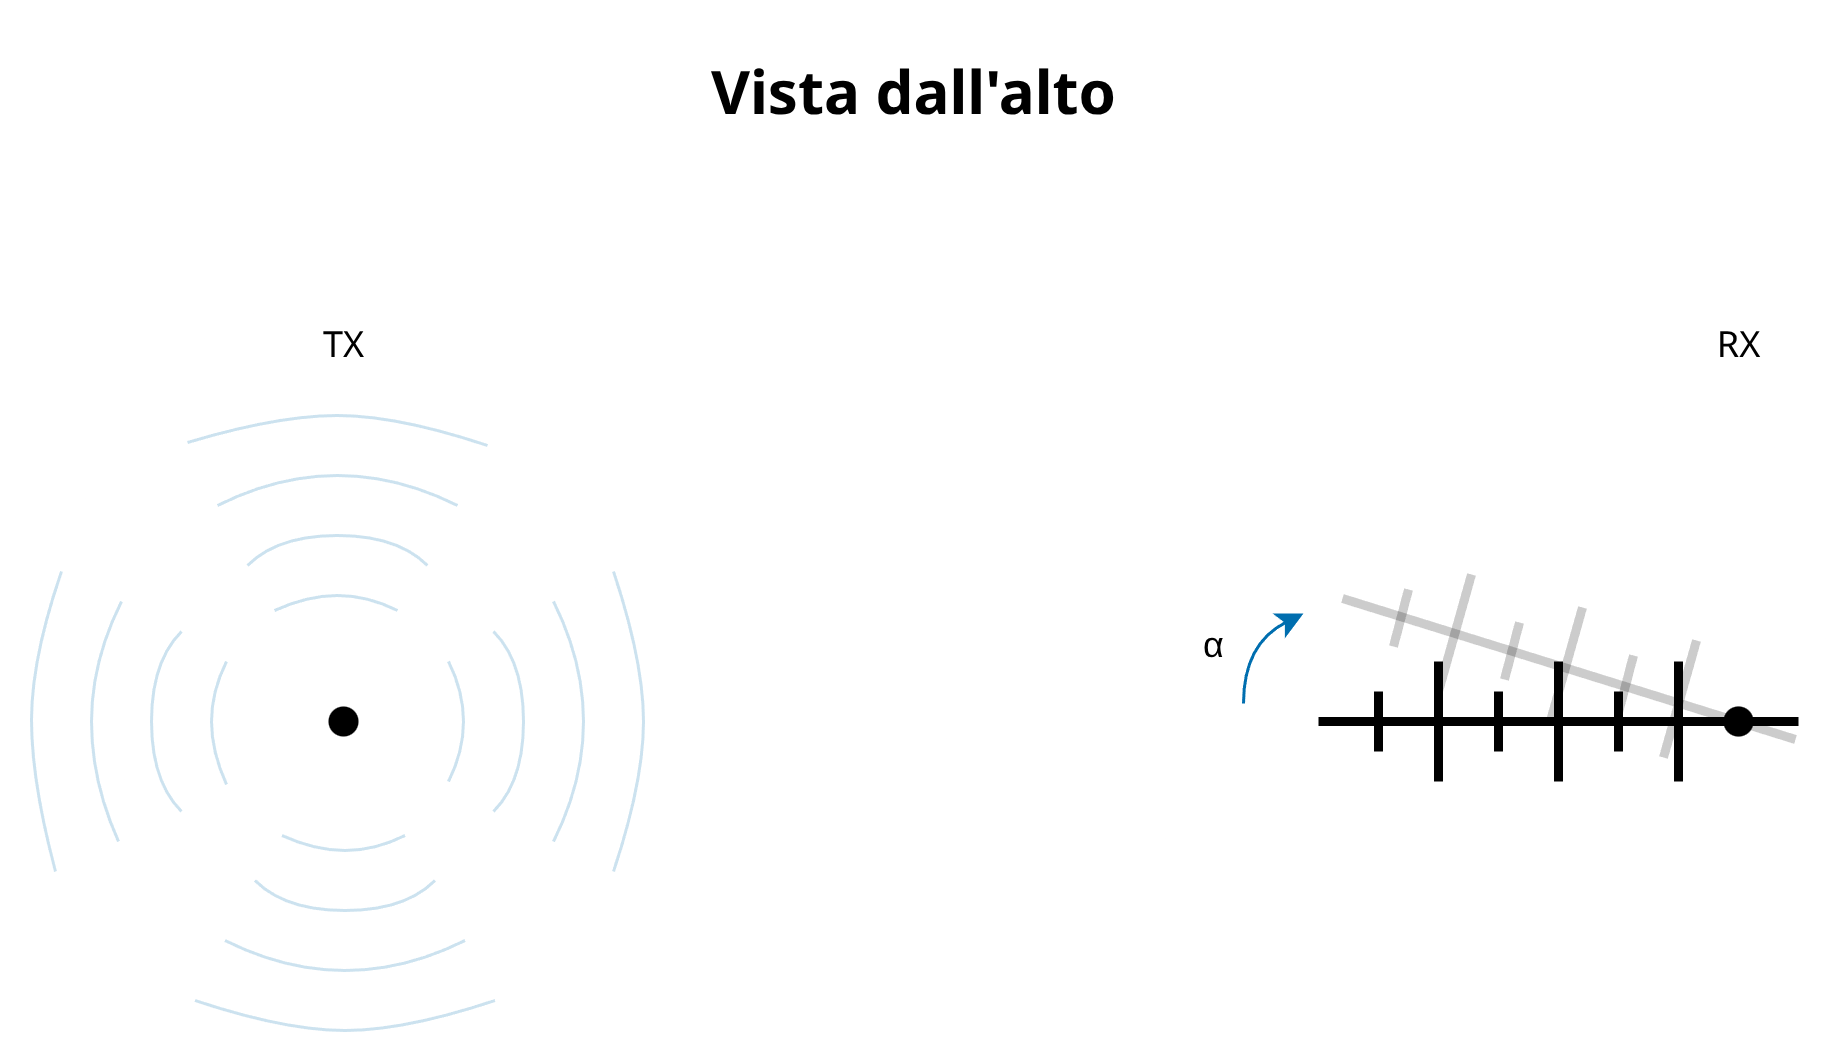
\includegraphics[width=0.6\textwidth]{img/tests/telemetry-test-direct.png}
    \caption{Test di disallineamento angolare dell'antenna direzionale.}
    \label{fig:directional-test}
\end{figure}
\newpage
\subsubsection{Disallineamento angolare dell'antenna omnidirezionale}
In seguito \'e stato eseguito lo stesso test, stavolta variando l'angolo di
disallineamento dell'antenna omnidirezionale sul piano verticale tra 0° e 30°,
e un ulteriore test a 90°, per simulare l'effetto della variazione di assetto
del razzo durante il volo.

\begin{figure}[H]
    \centering
    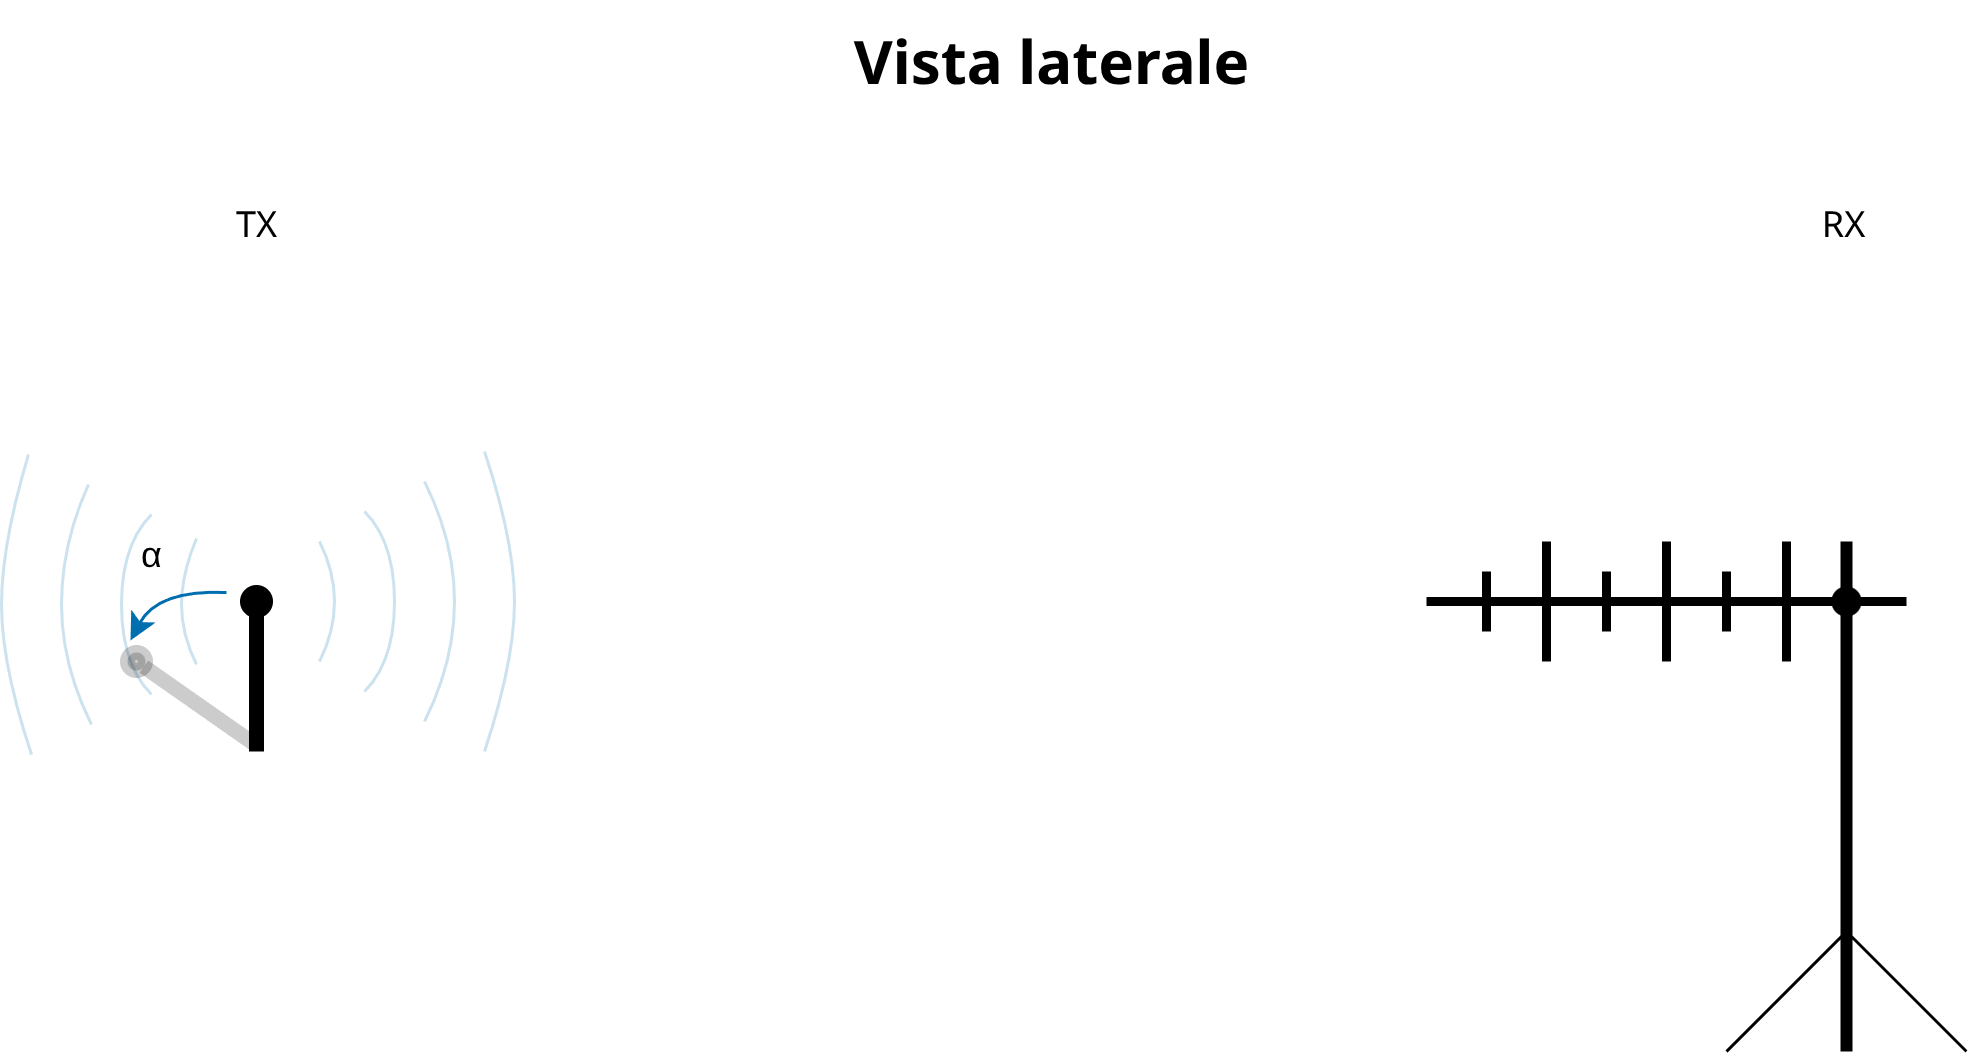
\includegraphics[width=0.6\textwidth]{img/tests/telemetry-test-omni.png}
    \caption{Test di disallineamento angolare dell'antenna omnidirezionale.}
    \label{fig:omnidirectional-test}
\end{figure}

\subsection{Test sul protocollo di comunicazione}
Dopo aver verificato le prestazioni dei moduli \ac{LoRa} e delle antenne, si è
proceduto a testare il protocollo di comunicazione implementato, valutando
l'affidabilità della trasmissione dei dati, la capacità di gestire la segmentazione
e la ricostruzione dei messaggi, e la robustezza del sistema in condizioni
di rumore e interferenze.
\subsubsection{Test del \emph{throughput}}
\ifdefined\HCode
    \begin{table}[H]
        \centering
        \resizebox{\textwidth}{!}{
            \begin{tabular}{|c|c|c|c|}
                \hline
                \textbf{Distanza} & \textbf{Frequenza di trasmissione} & \textbf{Potenza trasmissiva} & \textbf{Variabili di controllo} \\ \hline
                10m               & 873.125 MHz                        & +17 dBm                      & Dimensione del payload          \\ \hline
                50m               &                                    &                              &                                 \\ \hline
                100m              &                                    &                              &                                 \\ \hline
                150m              &                                    &                              &                                 \\ \hline
                200m              &                                    &                              &                                 \\ \hline
                250m              &                                    &                              &                                 \\ \hline
                500m              &                                    &                              &                                 \\ \hline
            \end{tabular}
        }
        \caption{Condizioni del test del throughput (HTML).}
        \label{tab:T1-conditions-html}
    \end{table}
\else
    \begin{table}[H]
        \centering
        \resizebox{\textwidth}{!}{
            \begin{tabular}{|c|c|c|c|}
                \hline
                \textbf{Distanza} & \textbf{Frequenza di trasmissione} & \textbf{Potenza trasmissiva} & \textbf{Variabili di controllo}         \\ \hline
                10m               & \multirow{7}{*}{873.125 MHz}       & \multirow{7}{*}{+17 dBm}     & \multirow{7}{*}{Dimensione del payload} \\ \cline{1-1}
                50m               &                                    &                              &                                         \\ \cline{1-1}
                100m              &                                    &                              &                                         \\ \cline{1-1}
                150m              &                                    &                              &                                         \\ \cline{1-1}
                200m              &                                    &                              &                                         \\ \cline{1-1}
                250m              &                                    &                              &                                         \\ \cline{1-1}
                500m              &                                    &                              &                                         \\ \hline
            \end{tabular}
        }
        \caption{Condizioni del test del throughput (PDF).}
        \label{tab:T1-conditions-pdf}
    \end{table}
\fi

\subsubsection{Test del \emph{throughput}}

Il test ha avuto l’obiettivo di misurare il \emph{throughput} effettivo del
sistema di telemetria, valutando la quantità di dati ricevuti correttamente al
variare della distanza tra le antenne, in condizioni ambientali reali.

Per ciascuna prova è stato trasmesso un \emph{payload} di dimensione fissa,
suddiviso in 5 \emph{chunk}, secondo il criterio di frammentazione descritto nel
Capitolo~\ref{chap:telemetry}.

\paragraph{Dettagli operativi del setup sperimentale}

Il test è stato eseguito in configurazione punto-punto, con l'antenna ricevente
mantenuta in posizione fissa, mentre l'antenna trasmittente
è stata progressivamente allontanata lungo una direttrice lineare, posizionandola
alle distanze indicate nella Tabella~\ref{tab:T1-conditions-pdf} e visibili nelle figure
\ref{fig:throughput-test-10-250m-full}-\ref{fig:throughput-test-500m}.

\begin{figure}[H]
    \centering
    \begin{minipage}{0.32\textwidth}
        \centering
        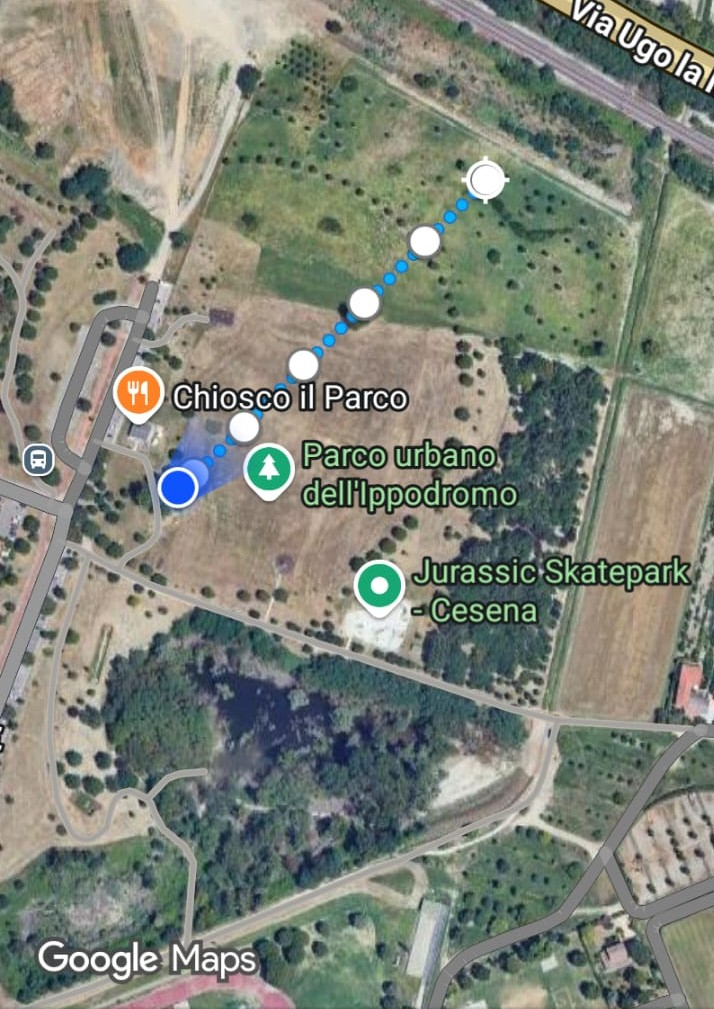
\includegraphics[width=\textwidth]{img/tests/T1/sat/10-250-full.jpeg}
        \caption{Posizioni di test da 10m a 250m con ostacoli.}
        \label{fig:throughput-test-10-250m-full}
    \end{minipage}
    \hfill
    \begin{minipage}{0.32\textwidth}
        \centering
        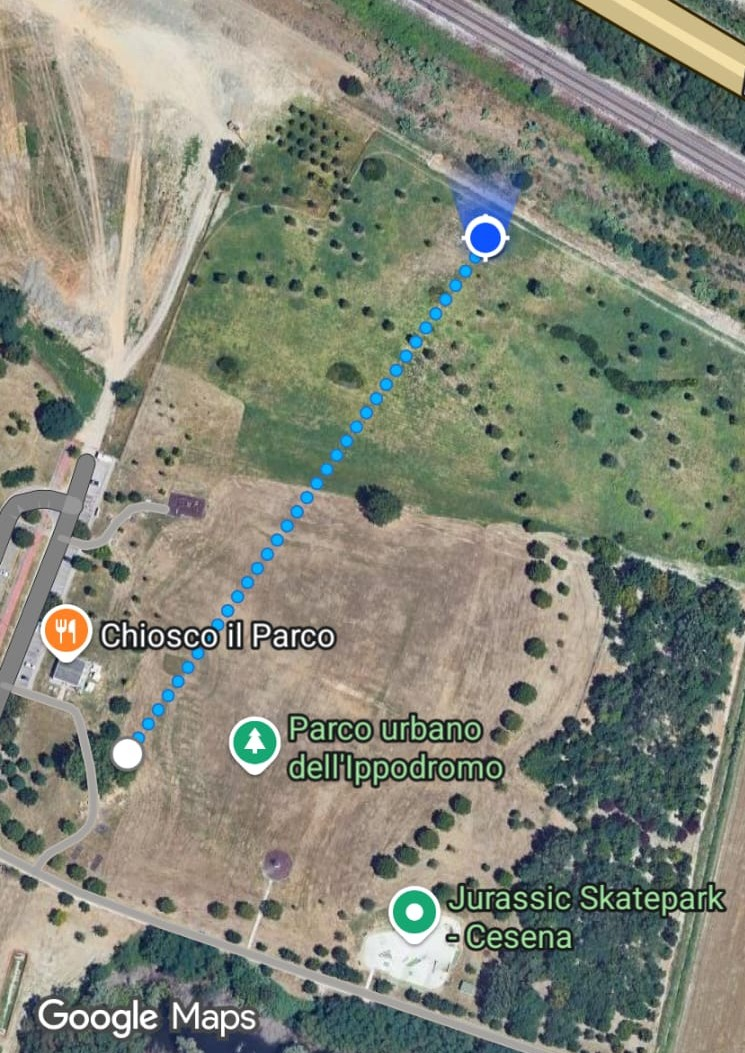
\includegraphics[width=\textwidth]{img/tests/T1/sat/10-250-direct.jpeg}
        \caption{Posizione di test a 250m senza ostacoli.}
        \label{fig:throughput-test-10-250m-direct}
    \end{minipage}
    \hfill
    \begin{minipage}{0.32\textwidth}
        \centering
        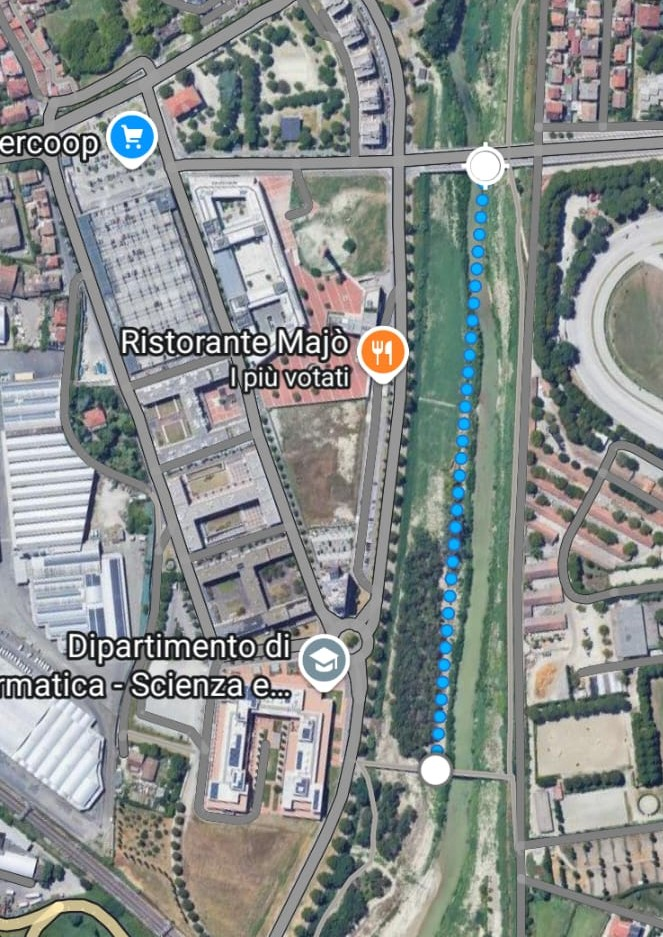
\includegraphics[width=\textwidth]{img/tests/T1/sat/500-full.jpeg}
        \caption{Posizione di test a 500m.}
        \label{fig:throughput-test-500m}
    \end{minipage}
\end{figure}

Per la distanza di 250~m sono state effettuate due misurazioni distinte:
\begin{itemize}
    \item \textbf{Scenario con ostacoli:} la trasmittente era posizionata dietro
          un leggero rilievo e fitta vegetazione, in assenza di linea di vista diretta (non-LoS);

    \item \textbf{Scenario parzialmente libero:} la trasmittente è stata spostata
          lateralmente di alcuni metri, ottenendo una visibilità migliorata, con la presenza
          di pochi alberi isolati lungo la traiettoria.
\end{itemize}

Il test alla distanza di 200~m è stato effettuato sulla cima di un piccolo rilievo naturale.

Il test alla distanza di 500~m è stato invece eseguito in una seconda location,
scelta per garantire una condizione di \emph{line of sight} (LoS) più favorevole:
la trasmissione è avvenuta tra due ponti stradali separati da un fiume, con l’antenna
ricevente posizionata su un ponte e la trasmittente sull'altro. Nonostante la presenza
di vegetazione lungo gli argini, la visibilità tra le antenne è rimasta sostanzialmente diretta.

Queste configurazioni hanno permesso di analizzare l'impatto reale degli ostacoli naturali
sulla qualità del collegamento radio e sul throughput risultante, mantenendo il
più possibile costanti le condizioni operative (altezza delle antenne, orientamento,
parametri di trasmissione).

Per ogni distanza, sono state misurate le seguenti metriche:
\begin{itemize}
    \item \ac{RSSI} medio rilevato;
    \item Numero di pacchetti ricevuti;
    \item Pacchetti al secondo (\emph{pkt/s});
    \item Byte al secondo (\emph{bps}) ricevuti correttamente.
\end{itemize}

\newpage
\subsubsection{Test sulla segmentazione e ricostruzione dei dati}
\begin{table}[H]
    \centering
    \resizebox{\textwidth}{!}{
        \begin{tabular}{|c|c|c|c|}
            \hline
            \textbf{Distanza} & \textbf{Frequenza di trasmissione} & \textbf{Potenza trasmissiva} & \textbf{Variabili di controllo} \\ \hline
            5m                & 873.125 MHz                        & +17 dBm                      & Dimensione del payload          \\ \hline
        \end{tabular}
    }
    \caption{Condizioni del test di segmentazione e ricostruzione dei dati.}
    \label{tab:T2-conditions}
\end{table}

Per valutare le prestazioni del protocollo di trasmissione nella gestione di pacchetti segmentati,
è stato condotto un test sperimentale mirato a misurare il tempo necessario alla ricostruzione
del \emph{payload} originale a partire dai \emph{chunk} ricevuti.

Il test è stato eseguito considerando \emph{payload} di dimensioni crescenti, suddivisi in 2, 3, 4 e 5
\emph{chunk}.
L’obiettivo era analizzare l’evoluzione del tempo medio di ricostruzione al variare del numero di
\emph{chunk}, al fine di valutare l’efficienza e la scalabilità del protocollo nella fase di riassemblaggio.

Questa analisi permette di valutare le prestazioni del sistema in scenari di trasmissione con pacchetti
di lunghezza variabile e di evidenziare eventuali criticità legate alla latenza introdotta dalla segmentazione.

Il tempo di ricostruzione di un pacchetto è calcolato come:

\begin{equation}
    \delta_{r} = (t_{UltimoChunk} - t_{PrimoChunk})
    \label{formula:reconstruction-time}
\end{equation}

\subsubsection{Test del meccanismo di \emph{drop}}
\begin{table}[H]
    \centering
    \resizebox{\textwidth}{!}{
        \begin{tabular}{|c|c|c|c|}
            \hline
            \textbf{Distanza} & \textbf{Frequenza di trasmissione} & \textbf{Potenza trasmissiva} & \textbf{Variabili di controllo}                      \\ \hline
            5m                & 873.125 MHz                        & +17 dBm                      & Frequenza di mancata trasmissione di un \emph{chunk} \\ \hline
        \end{tabular}
    }
    \caption{Condizioni del test del meccanismo di \emph{drop}.}
    \label{tab:T3-conditions}
\end{table}
La valutazione del meccanismo di \emph{drop} dei pacchetti è stata effettuata
per verificare la capacità del sistema di gestire situazioni in cui i pacchetti
ricevuti non sono completi o presentano errori di trasmissione.
Per eseguire il test, è stata simulata la mancata trasmissione di alcuni \emph{chunk}, consentendo di
verificare che il sistema identificasse e scartasse correttamente i pacchetti incompleti.

\subsubsection{Test del riordinamento dei pacchetti}
\begin{table}[H]
    \centering
    \resizebox{\textwidth}{!}{
        \begin{tabular}{|c|c|c|c|}
            \hline
            \textbf{Distanza} & \textbf{Frequenza di trasmissione} & \textbf{Potenza trasmissiva} & \textbf{Variabili di controllo}                 \\ \hline
            5m                & 873.125 MHz                        & +17 dBm                      & Frequenza di invio di \emph{chunk} fuori ordine \\ \hline
        \end{tabular}
    }
    \caption{Condizioni del test del meccanismo di riordinamento.}
    \label{tab:T4-conditions}
\end{table}
Per garantire l'integrit\'a dei dati, il protocollo mantiene i \emph{chunk} ricevuti
in una struttura dati ordinata.
Per verificare l'efficacia del meccanismo di riordinamento, sono stati inviati
alcuni \emph{chunk} in ordine invertito, consentendo di valutare la capacità del sistema
di riconoscere le sequenze fuori ordine, e riordinare i pacchetti prima della ricostruzione
del \emph{payload} originale.

\subsubsection{Test di robustezza e affidabilità}
\ifdefined\HCode
    \begin{table}[H]
        \centering
        \resizebox{\textwidth}{!}{
            \begin{tabular}{|c|c|c|c|}
                \hline
                \textbf{Distanza} & \textbf{Frequenza di trasmissione} & \textbf{Potenza trasmissiva} & \textbf{Variabili di controllo}                 \\ \hline
                5m                & 873.125 MHz                        & +17 dBm                      & Durata di trasmissione                          \\ \hline
                                  &                                    &                              & Dimensione del \emph{payload}                   \\ \hline
                                  &                                    &                              & Frequenza di trasmissione della seconda antenna \\ \hline
            \end{tabular}
        }
        \caption{Condizioni del test di robustezza e affidabilità.}
        \label{tab:T5-conditions-html}
    \end{table}
\else
    \begin{table}[H]
        \centering
        \resizebox{\textwidth}{!}{
            \begin{tabular}{|c|c|c|c|}
                \hline
                \textbf{Distanza}   & \textbf{Frequenza di trasmissione} & \textbf{Potenza trasmissiva} & \textbf{Variabili di controllo}                 \\ \hline
                \multirow{3}{*}{5m} & \multirow{3}{*}{873.125 MHz}       & \multirow{3}{*}{+17 dBm}     & Durata di trasmissione                          \\ \cline{4-4}
                                    &                                    &                              & Dimensione del \emph{payload}                   \\ \cline{4-4}
                                    &                                    &                              & Frequenza di trasmissione della seconda antenna \\ \hline
            \end{tabular}
        }
        \caption{Condizioni del test di robustezza e affidabilità.}
        \label{tab:T5-conditions-pdf}
    \end{table}
\fi
Per valutare la robustezza del sistema, sono stati condotti due test sperimentali.
Il primo ha riguardato la trasmissione di pacchetti in condizioni ottimali, a distanza
ravvicinata, con un \emph{payload} di dimensioni fisse, per verificare la stabilità
della comunicazione e studiare eventuali degradazioni delle prestazioni nel tempo.
Il test ha previsto l'invio di pacchetti frammentati per un periodo di 15 minuti,
monitorando la regolarità della trasmissione e il tempo di ricostruzione del \emph{payload} originale.

Il secondo test ha previsto l'attivazione di un secondo nodo trasmittente,
operante sulla stessa frequenza della prima antenna, per verificare eventuali effetti
di interferenze co-canalari. Il test è stato condotto nelle stesse condizioni del primo,
aggiungendo l'invio continuo di pacchetti da parte della seconda antenna.
I risultati dei due test sono stati successivamente confrontati per valutare l'effettivo impatto
delle interferenze sulla qualità del segnale e sulla stabilità della trasmissione.

\section{Ottimizzazioni apportate durante lo sviluppo}
\subsection{Compressione dei dati}
Considerando le limitazioni intrinseche dei moduli \ac{LoRa} utilizzati,
i tempi di ricostruzione osservati risultano comunque compatibili con i requisiti applicativi.
Per ridurre ulteriormente il carico trasmissivo, è stata implementata una compressione
delta per ridurre la dimensione complessiva dei \emph{payload} mantenendo inalterato il contenuto informativo.
\subsection{Gestione dei pacchetti}
Come discusso nella sezione \ref{sec:reconstruction-algorithm}, \'e stato implementato
un meccanismo di \emph{drop} dei pacchetti, che consente di scartare i pacchetti
incompleti o corrotti, evitando di accumulare dati parziali che potrebbero compromettere
le prestazioni e l'affidabilità del sistema.
Questo meccanismo si basa su un timeout configurabile, che permette di scartare i pacchetti
che non sono stati completati entro un certo intervallo di tempo, evitando l'accumulo
di dati inutili e garantendo una gestione efficiente della memoria.

Inoltre, per garantire l'integrità dei dati, il protocollo implementa un meccanismo di riordinamento
dei pacchetti, che consente di gestire situazioni in cui i \emph{chunk} arrivano
in ordine non sequenziale.

\chapter{Risultati e Analisi} \label{chap:results}

\section{Analisi dei dati raccolti durante le prove sperimentali}

\subsection{Risultati dei test preliminari}
I test preliminari hanno dimostrato che i moduli \ac{LoRa} EByte E220-900T22D
sono in grado di mantenere una comunicazione stabile anche in presenza di ostacoli naturali
(rilievi collinari, vegetazione) e artificiali, fino a distanze dell’ordine dei 2000 metri.
Questi risultati evidenziano la solidità della modulazione \ac{CSS}, in grado di garantire
una buona resilienza al rumore ambientale e alle interferenze radio locali.

Come mostrato in figura~\ref{fig:telemetry-misalignement}, anche con un disallineamento angolare
tra le antenne, l’intensità del segnale ricevuto è rimasta superiore al 60\% in tutti i casi testati,
con assenza di errori di decodifica o perdite significative di pacchetti.

I risultati sperimentali raccolti confermano la validità della scelta architetturale
adottata per il sistema radio, consentendo di procedere con lo sviluppo del
protocollo di comunicazione e della logica di trasmissione, assumendo una robusta
copertura anche in scenari \emph{outdoor} complessi.

\subsubsection{Disallineamento angolare dell'antenna direzionale}
\begin{table}[H]
    \centering
    \resizebox{0.8\textwidth}{!}{
        \begin{tabular}{|c|c|c|c|c|c|c|c|c|}
            \hline    \textbf{Distanza (m)} & \textbf{0°} & \textbf{5°} & \textbf{10°} & \textbf{15°} & \textbf{20°} & \textbf{25°} & \textbf{30°} & \textbf{90°} \\
            \hline    \textbf{100}          & 83.92       & 83.92       & 83.14        & 83.14        & 83.14        & 83.14        & 83.14        & 78.43        \\
            \hline    \textbf{250}          & 80.39       & 78.43       & 80.78        & 79.61        & 79.61        & 76.86        & 76.86        & 74.51        \\
            \hline    \textbf{780}          & 78.43       & 76.47       & 77.25        & 76.47        & 74.51        & 74.51        & 74.51        & 70.59        \\
            \hline    \textbf{1000}         & 69.02       & 68.63       & 66.67        & 65.49        & 68.63        & 71.37        & 71.37        & 69.80        \\
            \hline    \textbf{1500}         & 63.53       & 63.14       & 63.53        & 62.75        & 63.53        & 62.35        & 62.75        & 63.92        \\
            \hline    \textbf{2000}         & 62.75       & 62.75       & 62.75        & 63.14        & 62.75        & 63.14        & 62.75        & 62.75        \\
            \hline
        \end{tabular}
    }
    \caption{Intensità del segnale (\%) in funzione del disallineamento angolare dell'antenna direzionale e della distanza}
    \label{tab:signal-strength-directional}
\end{table}

\subsubsection{Disallineamento angolare dell'antenna omnidirezionale}
\begin{table}[H]
    \centering
    \resizebox{0.8\textwidth}{!}{
        \begin{tabular}{|c|c|c|c|c|c|c|c|c|}
            \hline    \textbf{Distanza (m)} & \textbf{0°} & \textbf{5°} & \textbf{10°} & \textbf{15°} & \textbf{20°} & \textbf{25°} & \textbf{30°} & \textbf{90°} \\
            \hline    \textbf{100}          & 80.00       & 78.43       & 77.65        & 78.43        & 80.39        & 82.35        & 82.35        & 84.31        \\
            \hline    \textbf{250}          & 76.47       & 79.61       & 79.61        & 78.43        & 78.43        & 78.82        & 78.82        & 82.35        \\
            \hline    \textbf{780}          & 73.73       & 72.55       & 69.80        & 72.55        & 72.94        & 73.73        & 71.37        & 76.47        \\
            \hline    \textbf{1000}         & 66.27       & 67.84       & 66.67        & 68.24        & 67.06        & 68.63        & 68.24        & 68.63        \\
            \hline    \textbf{1500}         & 62.75       & 62.75       & 63.14        & 62.75        & 62.35        & 62.35        & 62.35        & 64.71        \\
            \hline    \textbf{2000}         & 63.14       & 63.14       & 63.14        & 63.14        & 63.14        & 63.14        & 63.14        & 63.14        \\
            \hline
        \end{tabular}
    }
    \caption{Intensità del segnale (\%) in funzione del disallineamento angolare dell'antenna omnidirezionale e della distanza}
    \label{tab:signal-strength-omni}
\end{table}

\begin{figure}[H]
    \centering
    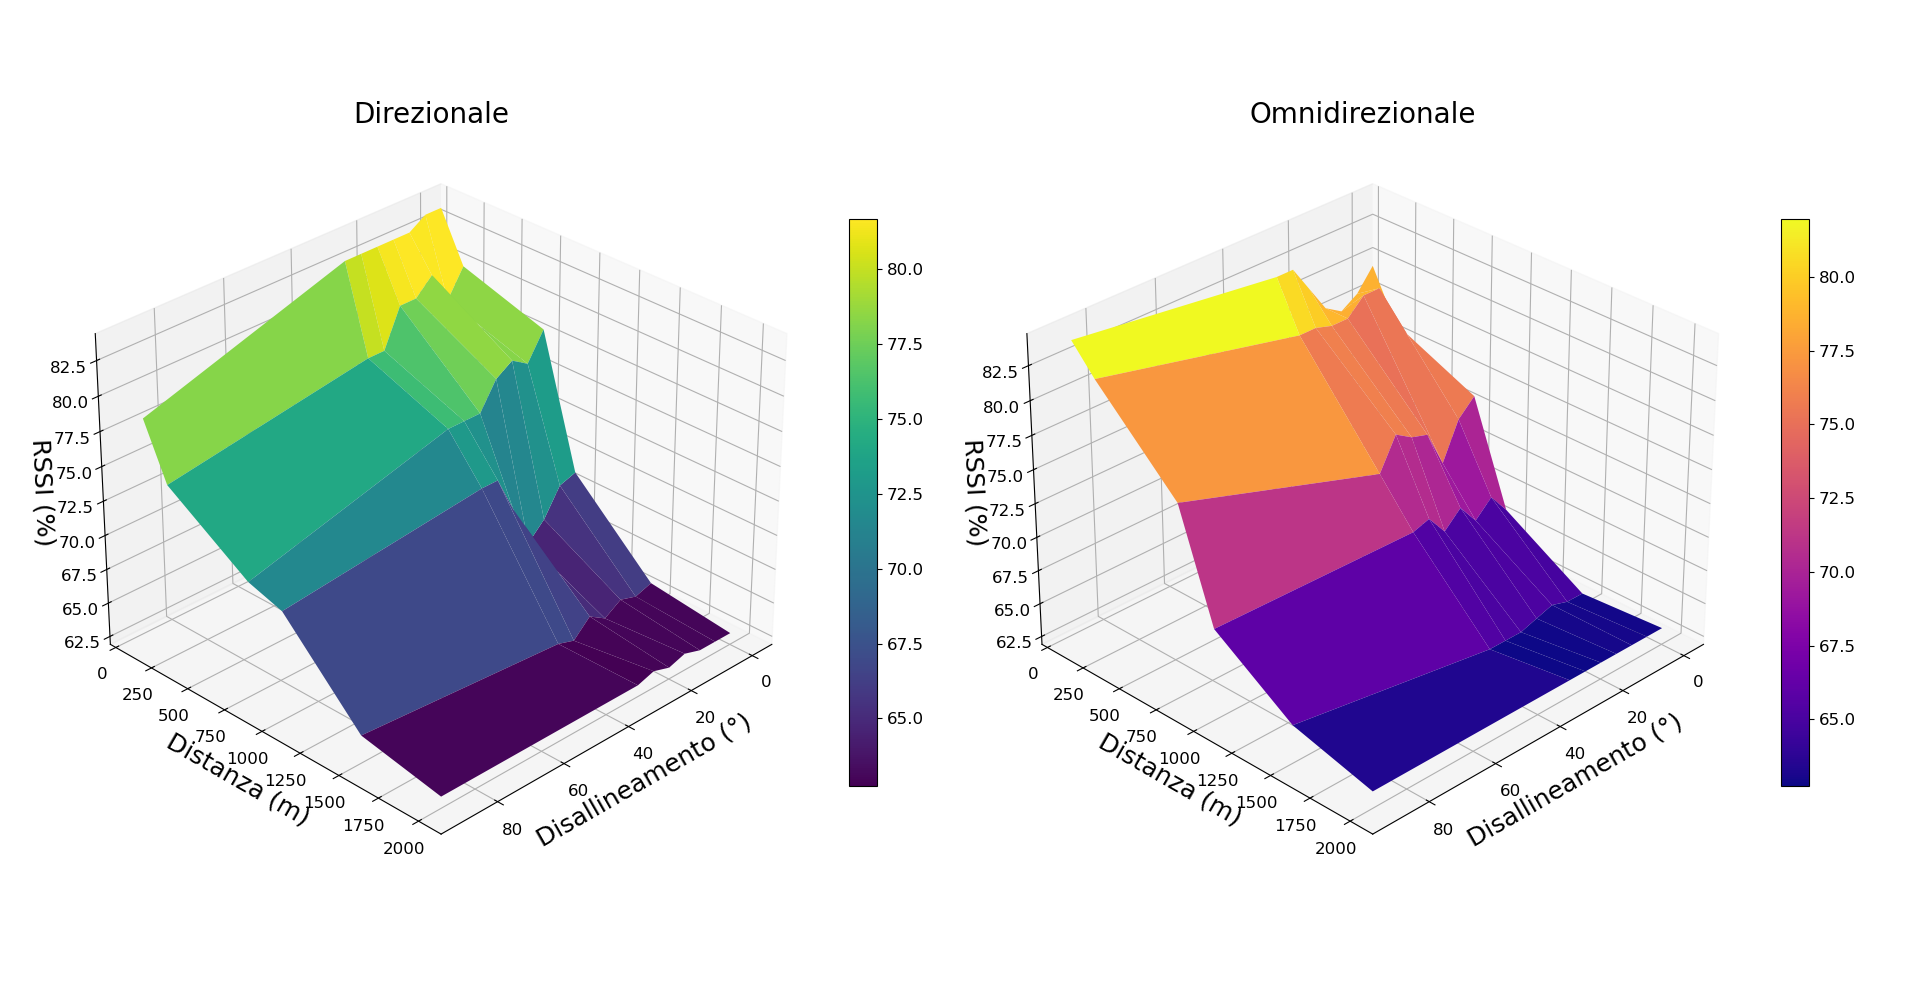
\includegraphics[width=0.95\textwidth]{img/tests/antenna-misalignement.png}
    \caption{Intensità del segnale in funzione della distanza e dell'angolo di disallineamento delle antenne.}
    \label{fig:telemetry-misalignement}
\end{figure}
\newpage
\subsection{Risultati dei test sul protocollo di comunicazione}
\subsubsection{Test del \emph{throughput}}
I risultati del test di \emph{throughput} indicano che il sistema di telemetria
mantiene prestazioni adeguate anche in condizioni operative complesse, con buona
robustezza alla variazione della distanza e alla presenza di ostacoli naturali.

Come riportato nella Tabella \ref{tab:T1-throughput_stats-pdf}, il throughput si è
mantenuto stabile (3.30 pkt/s e 646 B/s medi) per tutte le distanze testate, con
una leggera riduzione nello scenario a 250~m in presenza di ostacoli (vegetazione
e rilievi). In quel caso, la variabilità del throughput risulta più elevata
(deviazione standard: 10.85 B/s), confermando l'impatto degli ostacoli sulla
stabilità del collegamento. Al contrario, lo stesso scenario a 250~m con linea
di vista libera ha mostrato prestazioni sovrapponibili a quelle rilevate a 50–100–500~m.

\ifdefined\HCode
    \begin{table}[H]
        \centering
        \renewcommand{\arraystretch}{1.2}
        \begin{tabular}{|c|c|c|c|c|c|c|c|c|c|c|}
            \hline
            \textbf{Distanza} & \textbf{RSSI [\%] Mean} & \textbf{RSSI [\%] Std} & \textbf{RSSI [\%] Min} & \textbf{RSSI [\%] Max} & \textbf{Throughput [Byte/s] Mean} & \textbf{Throughput [Byte/s] Std} & \textbf{Throughput [Byte/s] Min} & \textbf{Throughput [Byte/s] Max} & \textbf{Pkt/s Mean} & \textbf{Pkt/s Std} \\
            \hline
            10 m              & 86.25                   & 0.54                   & 84.31                  & 87.84                  & 646.46                            & 0.19                             & 644.74                           & 646.86                           & 3.30                & 0.00               \\ \hline
            50 m              & 73.43                   & 0.78                   & 69.41                  & 75.29                  & 646.44                            & 0.16                             & 644.74                           & 646.86                           & 3.30                & 0.00               \\ \hline
            100 m             & 70.18                   & 0.86                   & 69.02                  & 71.76                  & 646.49                            & 0.09                             & 646.15                           & 646.86                           & 3.30                & 0.00               \\ \hline
            150 m             & 65.79                   & 1.73                   & 60.78                  & 69.02                  & 646.45                            & 0.15                             & 644.74                           & 646.86                           & 3.30                & 0.00               \\ \hline
            200 m             & 71.17                   & 1.15                   & 67.06                  & 72.94                  & 646.45                            & 0.07                             & 645.80                           & 646.86                           & 3.30                & 0.00               \\ \hline
            250 m (ostacoli)  & 64.90                   & 1.37                   & 60.39                  & 67.06                  & 634.54                            & 10.85                            & 587.71                           & 646.51                           & 3.24                & 0.06               \\ \hline
            250 m (libero)    & 65.21                   & 1.33                   & 59.61                  & 67.84                  & 646.49                            & 0.09                             & 646.44                           & 646.86                           & 3.30                & 0.00               \\ \hline
            500 m             & 73.64                   & 0.67                   & 71.76                  & 75.29                  & 646.42                            & 0.12                             & 644.74                           & 646.51                           & 3.30                & 0.00               \\ \hline
        \end{tabular}
        \caption{Statistiche sperimentali del throughput in funzione della distanza}
        \label{tab:T1-throughput_stats-html}
    \end{table}
\else
    \begin{table}[H]
        \centering
        \renewcommand{\arraystretch}{1.2}
        \resizebox{0.9\textwidth}{!}{
            \begin{tabular}{|c|cccc|cccc|cc|}
                \hline
                \textbf{Distanza} & \multicolumn{4}{c|}{\textbf{RSSI [\%]}} & \multicolumn{4}{c|}{\textbf{Throughput [Byte/s]}} & \multicolumn{2}{c|}{\textbf{Pkt/s}}                                                                 \\
                \cline{2-11}
                                  & \textbf{Mean}                           & \textbf{Std}                                      & \textbf{Min}                        & \textbf{Max}
                                  & \textbf{Mean}                           & \textbf{Std}                                      & \textbf{Min}                        & \textbf{Max}
                                  & \textbf{Mean}                           & \textbf{Std}                                                                                                                                            \\
                \hline
                10 m              & 86.25                                   & 0.54                                              & 84.31                               & 87.84        & 646.46 & 0.19  & 644.74 & 646.86 & 3.30 & 0.00 \\ \hline
                50 m              & 73.43                                   & 0.78                                              & 69.41                               & 75.29        & 646.44 & 0.16  & 644.74 & 646.86 & 3.30 & 0.00 \\ \hline
                100 m             & 70.18                                   & 0.86                                              & 69.02                               & 71.76        & 646.49 & 0.09  & 646.15 & 646.86 & 3.30 & 0.00 \\ \hline
                150 m             & 65.79                                   & 1.73                                              & 60.78                               & 69.02        & 646.45 & 0.15  & 644.74 & 646.86 & 3.30 & 0.00 \\ \hline
                200 m             & 71.17                                   & 1.15                                              & 67.06                               & 72.94        & 646.45 & 0.07  & 645.80 & 646.86 & 3.30 & 0.00 \\ \hline
                250 m (ostacoli)  & 64.90                                   & 1.37                                              & 60.39                               & 67.06        & 634.54 & 10.85 & 587.71 & 646.51 & 3.24 & 0.06 \\ \hline
                250 m (libero)    & 65.21                                   & 1.33                                              & 59.61                               & 67.84        & 646.49 & 0.09  & 646.44 & 646.86 & 3.30 & 0.00 \\ \hline
                500 m             & 73.64                                   & 0.67                                              & 71.76                               & 75.29        & 646.42 & 0.12  & 644.74 & 646.51 & 3.30 & 0.00 \\ \hline
            \end{tabular}
        }
        \caption{Statistiche sperimentali del throughput in funzione della distanza}
        \label{tab:T1-throughput_stats-pdf}
    \end{table}
\fi
La qualità del segnale, rappresentata dal valore di \ac{RSSI}, è risultata elevata
in tutti i test, con valori medi sempre superiori al 65\%, ad eccezione della
configurazione 250~m con ostacoli. La Figura~\ref{fig:throughput-rssi-dist-regression}
mostra l’andamento dell’RSSI medio in funzione della distanza, con una regressione
logaritmica che evidenzia un lieve decadimento complessivo all’aumentare della distanza.
Il boxplot in Figura~\ref{fig:throughput-rssi-dist-box} evidenzia inoltre un’anomala
crescita del valore medio dell’RSSI a 200~m, attribuibile alla posizione sopraelevata
della trasmittente in quel punto, causata dalla conformazione naturale del terreno.

\begin{figure}[H]
    \centering
    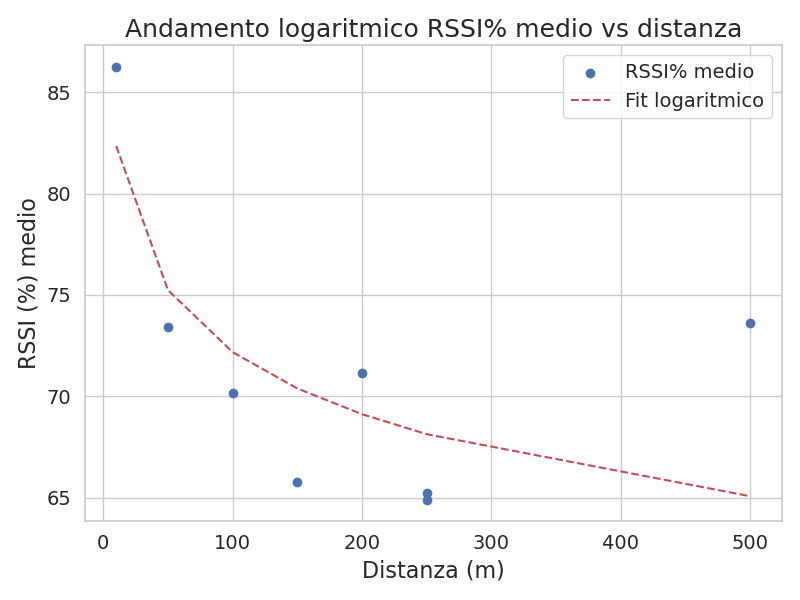
\includegraphics[width=0.8\textwidth]{img/tests/T1/T1-rssi_dist_regression.png}
    \caption{Andamento dell'RSSI in funzione della distanza (regressione logaritmica).}
    \label{fig:throughput-rssi-dist-regression}
\end{figure}

\begin{figure}[H]
    \centering
    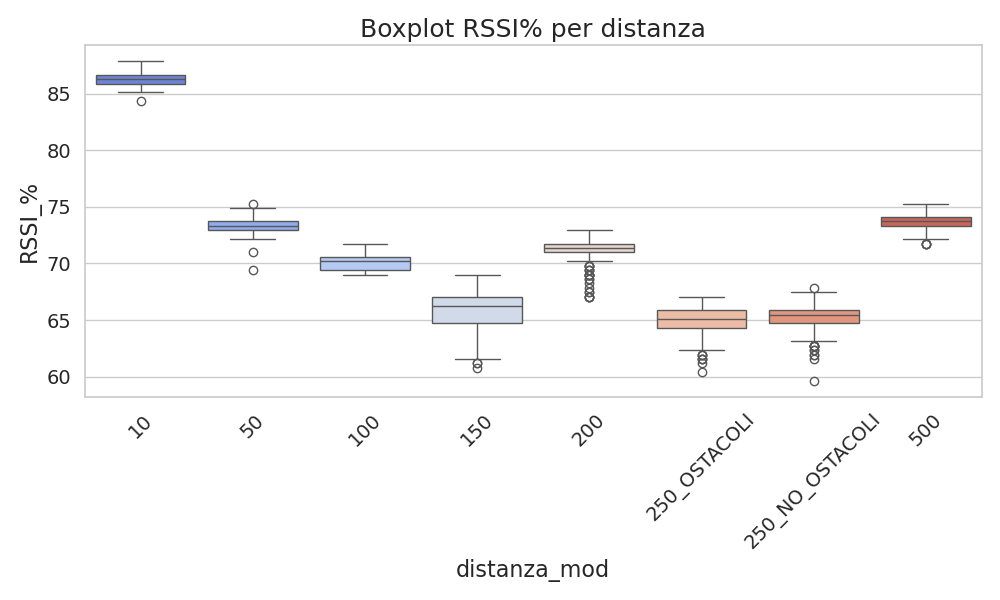
\includegraphics[width=0.9\textwidth]{img/tests/T1/T1-rssi_dist_box.png}
    \caption{Distribuzione (boxplot) dell'RSSI per ciascuna distanza testata.}
    \label{fig:throughput-rssi-dist-box}
\end{figure}
\newpage
L’impatto degli ostacoli naturali è ancora più evidente osservando il comportamento
del throughput. La Figura~\ref{fig:rssi-throughput-scat} mostra la dispersione dei
valori di throughput in funzione della distanza: nello scenario con ostacoli a 250~m
si osserva una maggiore variabilità e una riduzione rispetto alla configurazione
equivalente con linea di vista. La Figura~\ref{fig:RSSI-throughput-dist} mette a
confronto l’RSSI e il throughput medi per ciascuna distanza, evidenziando la coerenza
tra decadimento del segnale e leggera riduzione delle prestazioni.

\begin{figure}[H]
    \centering
    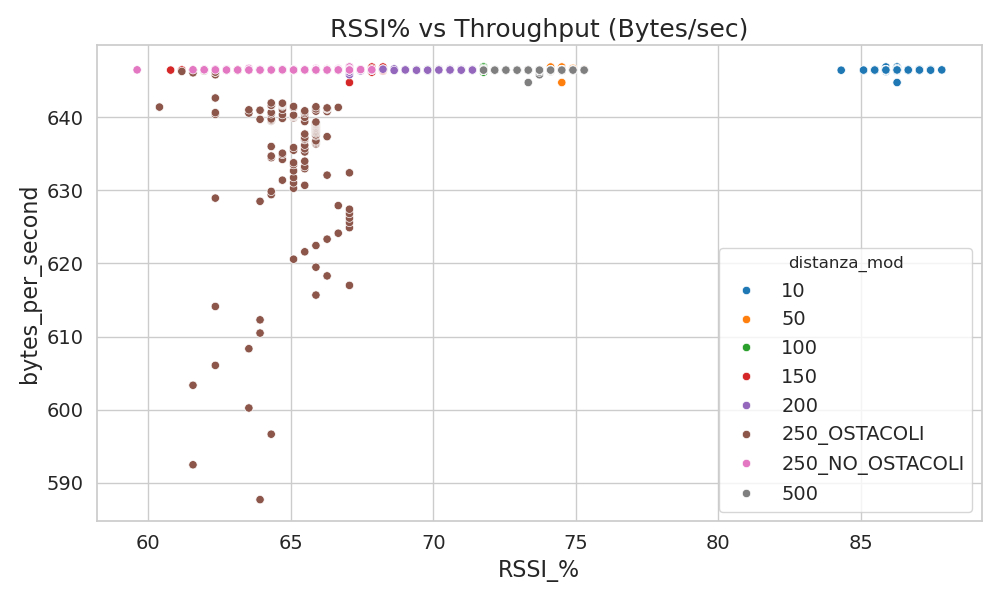
\includegraphics[width=0.8\textwidth]{img/tests/T1/T1-rssi_throughput_scat.png}
    \caption{Throughput in funzione della distanza (distribuzione puntuale).}
    \label{fig:rssi-throughput-scat}
\end{figure}

\begin{figure}[H]
    \centering
    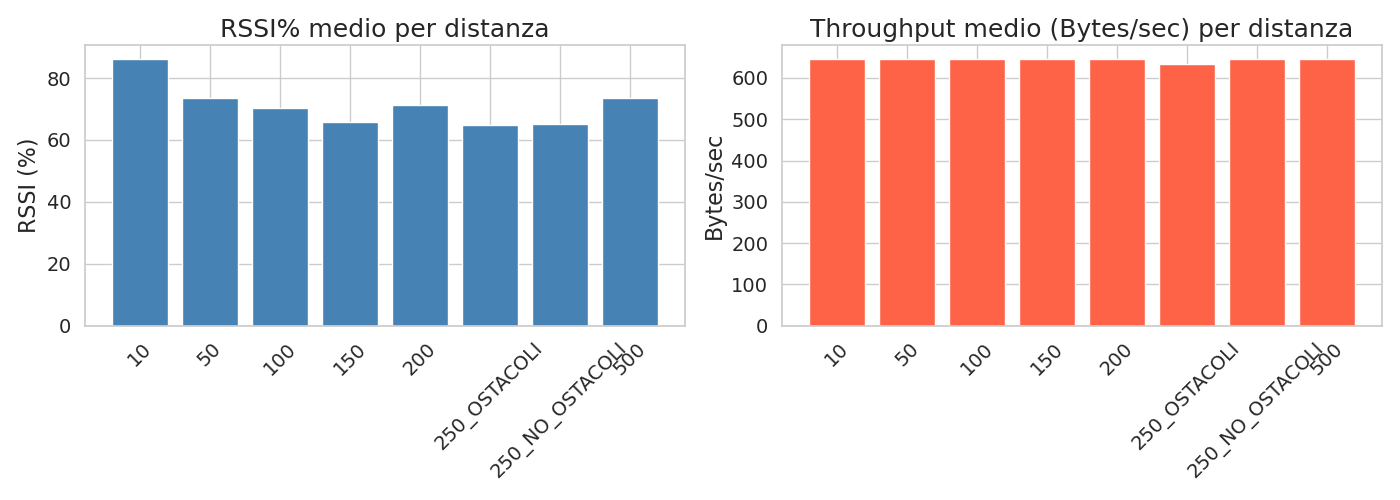
\includegraphics[width=0.8\textwidth]{img/tests/T1/T1-rssi_throughput_col.png}
    \caption{RSSI e throughput medi in funzione della distanza.}
    \label{fig:RSSI-throughput-dist}
\end{figure}

In conclusione, anche nello scenario con ostacoli a 250~m, il degrado delle prestazioni
è risultato contenuto e non critico: il throughput medio si è mantenuto sopra i
3.2 pkt/s, dimostrando una buona resilienza del sistema alla degradazione del canale radio.

\subsubsection{Test sulla segmentazione e ricostruzione dei dati}
I risultati dei test confermano che il sistema gestisce correttamente il riassemblaggio
dei \emph{payload} segmentati, con un tempo medio di ricostruzione che cresce in
maniera approssimativamente lineare con il numero di \emph{chunk}, come mostrato
in figura~\ref{fig:segmentation-reconstruction-avg-time}.

Come evidenziato in figura~\ref{fig:segmentation-reconstruction-sd}, la deviazione standard
dei tempi di ricostruzione si mantiene relativamente stabile al variare del numero di \emph{chunk},
indicando una buona prevedibilità temporale del processo di riassemblaggio.

Le distribuzioni dei tempi di ricostruzione (figure~\ref{fig:segmentation-test-2chunks}–\ref{fig:segmentation-test-5chunks})
mostrano che i tempi di ricostruzione sono concentrati attorno a valori medi, con una
leggera variabilità, ma senza picchi significativi.

\begin{figure}[H]
    \centering
    \begin{minipage}{0.47\textwidth}
        \centering
        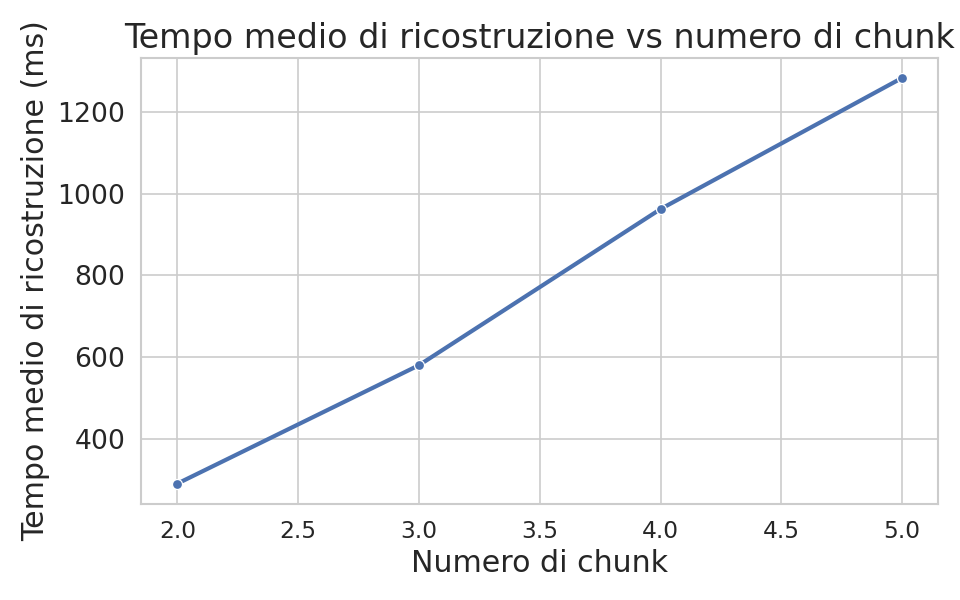
\includegraphics[width=\textwidth]{img/tests/T2/T2-avg-time.png}
        \caption{Tempo medio di ricostruzione per numero di chunk.}
        \label{fig:segmentation-reconstruction-avg-time}
    \end{minipage}
    \hfill
    \begin{minipage}{0.47\textwidth}
        \centering
        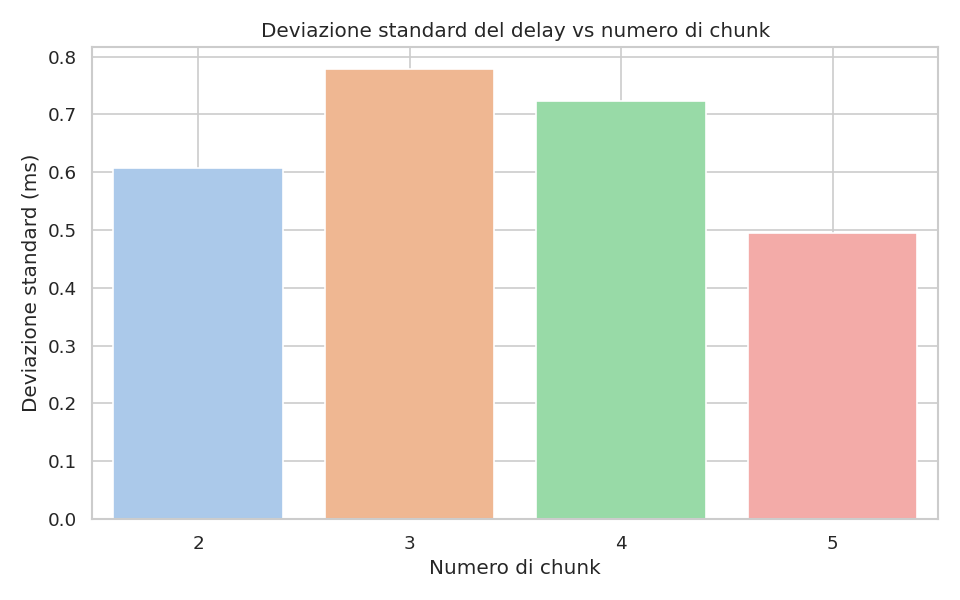
\includegraphics[width=\textwidth]{img/tests/T2/T2-sd.png}
        \caption{Deviazione standard dei tempi di ricostruzione per numero di chunk.}
        \label{fig:segmentation-reconstruction-sd}
    \end{minipage}
\end{figure}

\begin{figure}[H]
    \centering
    \begin{minipage}{0.47\textwidth}
        \centering
        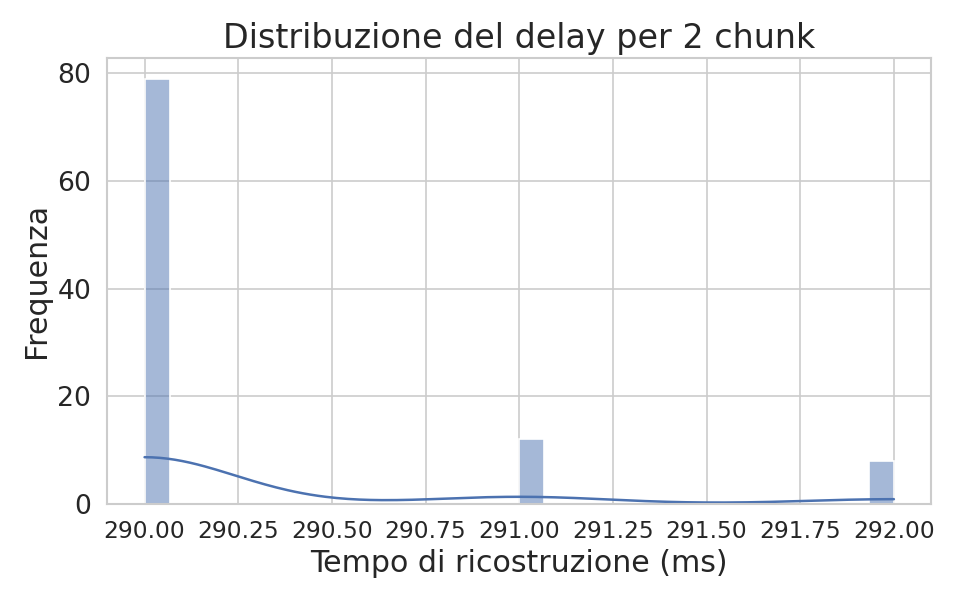
\includegraphics[width=\textwidth]{img/tests/T2/T2-dist-2chunks.png}
        \caption{Distribuzione dei tempi di ricostruzione per 2 chunk}
        \label{fig:segmentation-test-2chunks}
    \end{minipage}
    \hfill
    \begin{minipage}{0.47\textwidth}
        \centering
        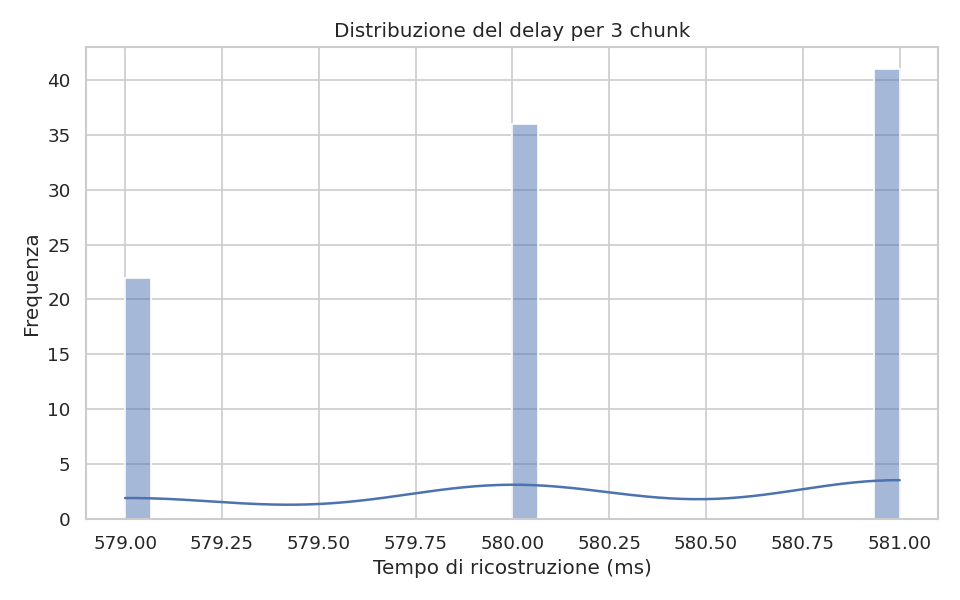
\includegraphics[width=\textwidth]{img/tests/T2/T2-dist-3chunks.png}
        \caption{Distribuzione dei tempi di ricostruzione per 3 chunk}
        \label{fig:segmentation-test-3chunks}
    \end{minipage}

    \vspace{1cm}

    \begin{minipage}{0.47\textwidth}
        \centering
        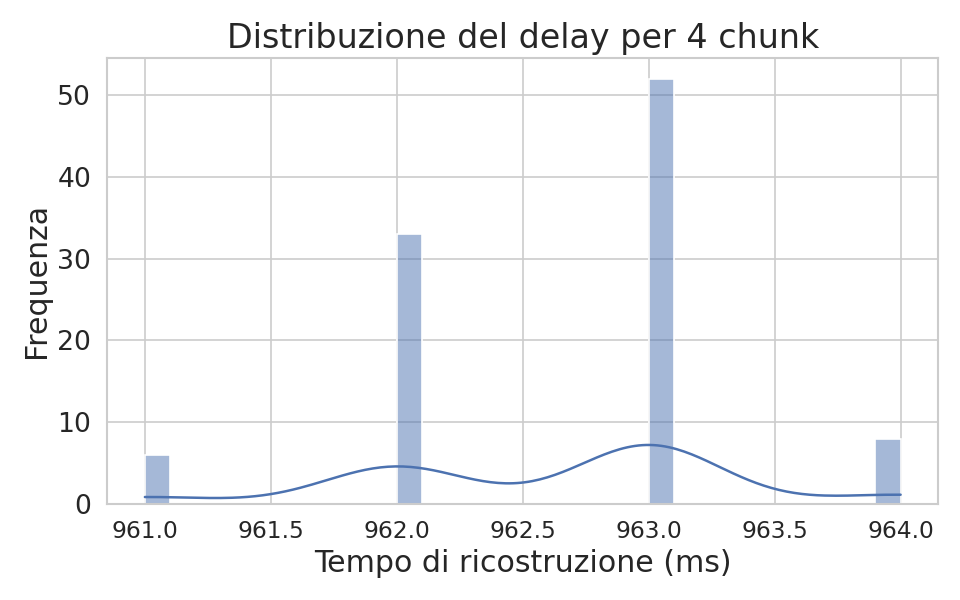
\includegraphics[width=\textwidth]{img/tests/T2/T2-dist-4chunks.png}
        \caption{Distribuzione dei tempi di ricostruzione per 4 chunk}
        \label{fig:segmentation-test-4chunks}
    \end{minipage}
    \hfill
    \begin{minipage}{0.47\textwidth}
        \centering
        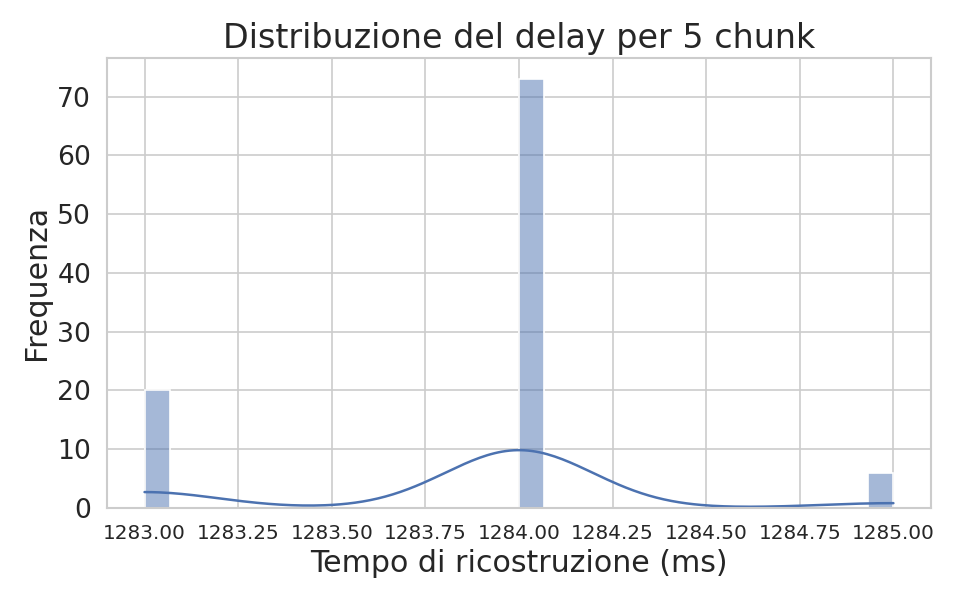
\includegraphics[width=\textwidth]{img/tests/T2/T2-dist-5chunks.png}
        \caption{Distribuzione dei tempi di ricostruzione per 5 chunk}
        \label{fig:segmentation-test-5chunks}
    \end{minipage}
\end{figure}
\newpage
\subsubsection{Test del meccanismo di \emph{drop}}
Il meccanismo di \emph{drop} si \'e dimostrato efficace nel gestire l'arrivo di pacchetti
non validi o incompleti, evitando l'accumulo di dati parziali, garantendo un'efficace
gestione della memoria e delle risorse.
La simulazione prevedeva l'invio di pacchetti frammentati, con la perdita di un \emph{chunk}
ogni 3 pacchetti, con una percentuale di perdita prevista del 33\%.
I risultati ottenuti sono riportati nella tabella~\ref{tab:loss_rate}, che conferma la
percentuale di perdita dei pacchetti attesa.

\begin{table}[H]
    \centering
    \resizebox{\textwidth}{!}{
        \begin{tabular}{|c|c|c|c|c|}
            \hline
            \textbf{Tempo} & \textbf{\emph{Loss Rate} (\%)} & \textbf{\emph{Packet Number}} & \textbf{Pacchetti ricevuti} & \textbf{Pacchetti scartati} \\
            \hline
            00:00:000      & 33,33                          & 3                             & 3                           & 1                           \\ \hline
            00:04:359      & 33,33                          & 6                             & 6                           & 2                           \\ \hline
            00:08:720      & 33,33                          & 9                             & 9                           & 3                           \\ \hline
            00:13:080      & 33,33                          & 12                            & 12                          & 4                           \\ \hline
            00:17:440      & 33,33                          & 15                            & 15                          & 5                           \\ \hline
            00:21:803      & 33,33                          & 18                            & 18                          & 6                           \\ \hline
            00:26:166      & 33,33                          & 21                            & 21                          & 7                           \\ \hline
            00:30:528      & 33,33                          & 24                            & 24                          & 8                           \\ \hline
            00:39:255      & 33,33                          & 30                            & 30                          & 10                          \\ \hline
            00:43:617      & 33,33                          & 33                            & 33                          & 11                          \\ \hline
            00:47:980      & 33,33                          & 36                            & 36                          & 12                          \\ \hline
            00:52:343      & 33,33                          & 39                            & 39                          & 13                          \\ \hline
            00:56:706      & 33,33                          & 42                            & 42                          & 14                          \\ \hline
            01:01:069      & 33,33                          & 45                            & 45                          & 15                          \\ \hline
            01:05:433      & 33,33                          & 48                            & 48                          & 16                          \\ \hline
            01:09:795      & 33,33                          & 51                            & 51                          & 17                          \\ \hline
            01:14:158      & 33,33                          & 54                            & 54                          & 18                          \\ \hline
            01:18:521      & 33,33                          & 57                            & 57                          & 19                          \\ \hline
            01:22:884      & 33,33                          & 60                            & 60                          & 20                          \\ \hline
            01:27:248      & 33,33                          & 63                            & 63                          & 21                          \\ \hline
            01:31:611      & 33,33                          & 66                            & 66                          & 22                          \\ \hline
            01:35:973      & 33,33                          & 69                            & 69                          & 23                          \\ \hline
            01:40:336      & 33,33                          & 72                            & 72                          & 24                          \\ \hline
            01:44:700      & 33,33                          & 75                            & 75                          & 25                          \\ \hline
            01:49:063      & 33,33                          & 78                            & 78                          & 26                          \\ \hline
            01:53:425      & 33,33                          & 81                            & 81                          & 27                          \\ \hline
            01:57:789      & 33,33                          & 84                            & 84                          & 28                          \\ \hline
            02:02:152      & 33,33                          & 87                            & 87                          & 29                          \\ \hline
            02:06:514      & 33,33                          & 90                            & 90                          & 30                          \\ \hline
        \end{tabular}
    }
    \caption{Tasso di perdita dei pacchetti durante il test del meccanismo di \emph{drop}.}
    \label{tab:loss_rate}
\end{table}
\newpage
\subsubsection{Test del riordinamento dei pacchetti}
Il test di riordinamento dei pacchetti ha dimostrato che il sistema è in grado di
riconoscere e gestire correttamente i \emph{chunk} ricevuti in ordine sparso,
riordinandoli in base al loro \emph{Chunk Number} prima della ricostruzione del \emph{payload} originale.
I risultati sono riportati nella tabella~\ref{tab:chunk_order}, che mostra l'ordine
di arrivo dei pacchetti, e lo stato di ordinamento per ogni sequenza di \emph{chunk}.
Come nel test precedente, la simulazione prevedeva l'invio di pacchetti frammentati,
con lo scambio dell'ordine di arrivo di due \emph{chunk} ogni 3 pacchetti.

\begin{table}[H]
    \centering
    \resizebox{\textwidth}{!}{
        \begin{tabular}{|c|c|c|c|c|c|}
            \hline
            \textbf{Tempo} & \textbf{\emph{Packet Number}} & \textbf{\emph{Total Chunks}} & \textbf{\emph{Chunk} ricevuti} & \textbf{Ordinati} & \textbf{Ordine di arrivo} \\
            \hline
            00:00:000      & 1                             & 5                            & 5                              & YES               & 1-2-3-4-5                 \\ \hline
            00:03:101      & 2                             & 5                            & 5                              & YES               & 1-2-3-4-5                 \\ \hline
            00:04:652      & 3                             & 5                            & 5                              & NO                & 1-3-2-4-5                 \\ \hline
            00:06:203      & 4                             & 5                            & 5                              & YES               & 1-2-3-4-5                 \\ \hline
            00:07:753      & 5                             & 5                            & 5                              & YES               & 1-2-3-4-5                 \\ \hline
            00:09:305      & 6                             & 5                            & 5                              & NO                & 1-3-2-4-5                 \\ \hline
            00:10:856      & 7                             & 5                            & 5                              & YES               & 1-2-3-4-5                 \\ \hline
            00:12:407      & 8                             & 5                            & 5                              & YES               & 1-2-3-4-5                 \\ \hline
            00:13:958      & 9                             & 5                            & 5                              & NO                & 1-3-2-4-5                 \\ \hline
            00:15:509      & 10                            & 5                            & 5                              & YES               & 1-2-3-4-5                 \\ \hline
            00:17:059      & 11                            & 5                            & 5                              & YES               & 1-2-3-4-5                 \\ \hline
            00:18:610      & 12                            & 5                            & 5                              & NO                & 1-3-2-4-5                 \\ \hline
            00:20:161      & 13                            & 5                            & 5                              & YES               & 1-2-3-4-5                 \\ \hline
            00:21:712      & 14                            & 5                            & 5                              & YES               & 1-2-3-4-5                 \\ \hline
            00:23:264      & 15                            & 5                            & 5                              & YES               & 1-2-3-4-5                 \\ \hline
            00:24:815      & 16                            & 5                            & 5                              & NO                & 1-3-2-4-5                 \\ \hline
            00:26:366      & 17                            & 5                            & 5                              & YES               & 1-2-3-4-5                 \\ \hline
            00:27:916      & 18                            & 5                            & 5                              & NO                & 1-3-2-4-5                 \\ \hline
            00:29:468      & 19                            & 5                            & 5                              & YES               & 1-2-3-4-5                 \\ \hline
            00:31:019      & 20                            & 5                            & 5                              & YES               & 1-2-3-4-5                 \\ \hline
            00:32:569      & 21                            & 5                            & 5                              & NO                & 1-3-2-4-5                 \\ \hline
            00:34:121      & 22                            & 5                            & 5                              & YES               & 1-2-3-4-5                 \\ \hline
            00:35:671      & 23                            & 5                            & 5                              & YES               & 1-2-3-4-5                 \\ \hline
            00:37:223      & 24                            & 5                            & 5                              & YES               & 1-2-3-4-5                 \\ \hline
            00:38:773      & 25                            & 5                            & 5                              & YES               & 1-2-3-4-5                 \\ \hline
            00:40:325      & 26                            & 5                            & 5                              & YES               & 1-2-3-4-5                 \\ \hline
            00:41:875      & 27                            & 5                            & 5                              & YES               & 1-2-3-4-5                 \\ \hline
            00:43:426      & 28                            & 5                            & 5                              & YES               & 1-2-3-4-5                 \\ \hline
            00:44:978      & 29                            & 5                            & 5                              & YES               & 1-2-3-4-5                 \\ \hline
            00:46:529      & 30                            & 5                            & 5                              & NO                & 1-3-2-4-5                 \\
            \hline
        \end{tabular}
    }
    \caption{Verifica dell'ordine di arrivo dei chunk per ogni pacchetto}
    \label{tab:chunk_order}
\end{table}
\newpage
\subsubsection{Test di robustezza e affidabilità}
Il primo test di robustezza ha permesso di verificare che il sistema è in grado
di mantenere una comunicazione stabile e affidabile anche per periodi prolungati,
senza cali di prestazioni né perdite di pacchetti.

I risultati mostrano che il sistema ha mantenuto un livello di prestazioni costante
per tutta la durata dell'esperimento, evidenziato dalla crescita lineare del
numero di pacchetti ricevuti e dalla stabilità del tempo di ricostruzione del
\emph{payload} originale, come illustrato nella figura~\ref{fig:telemetry-robustness-test}.

\begin{figure}[H]
    \centering
    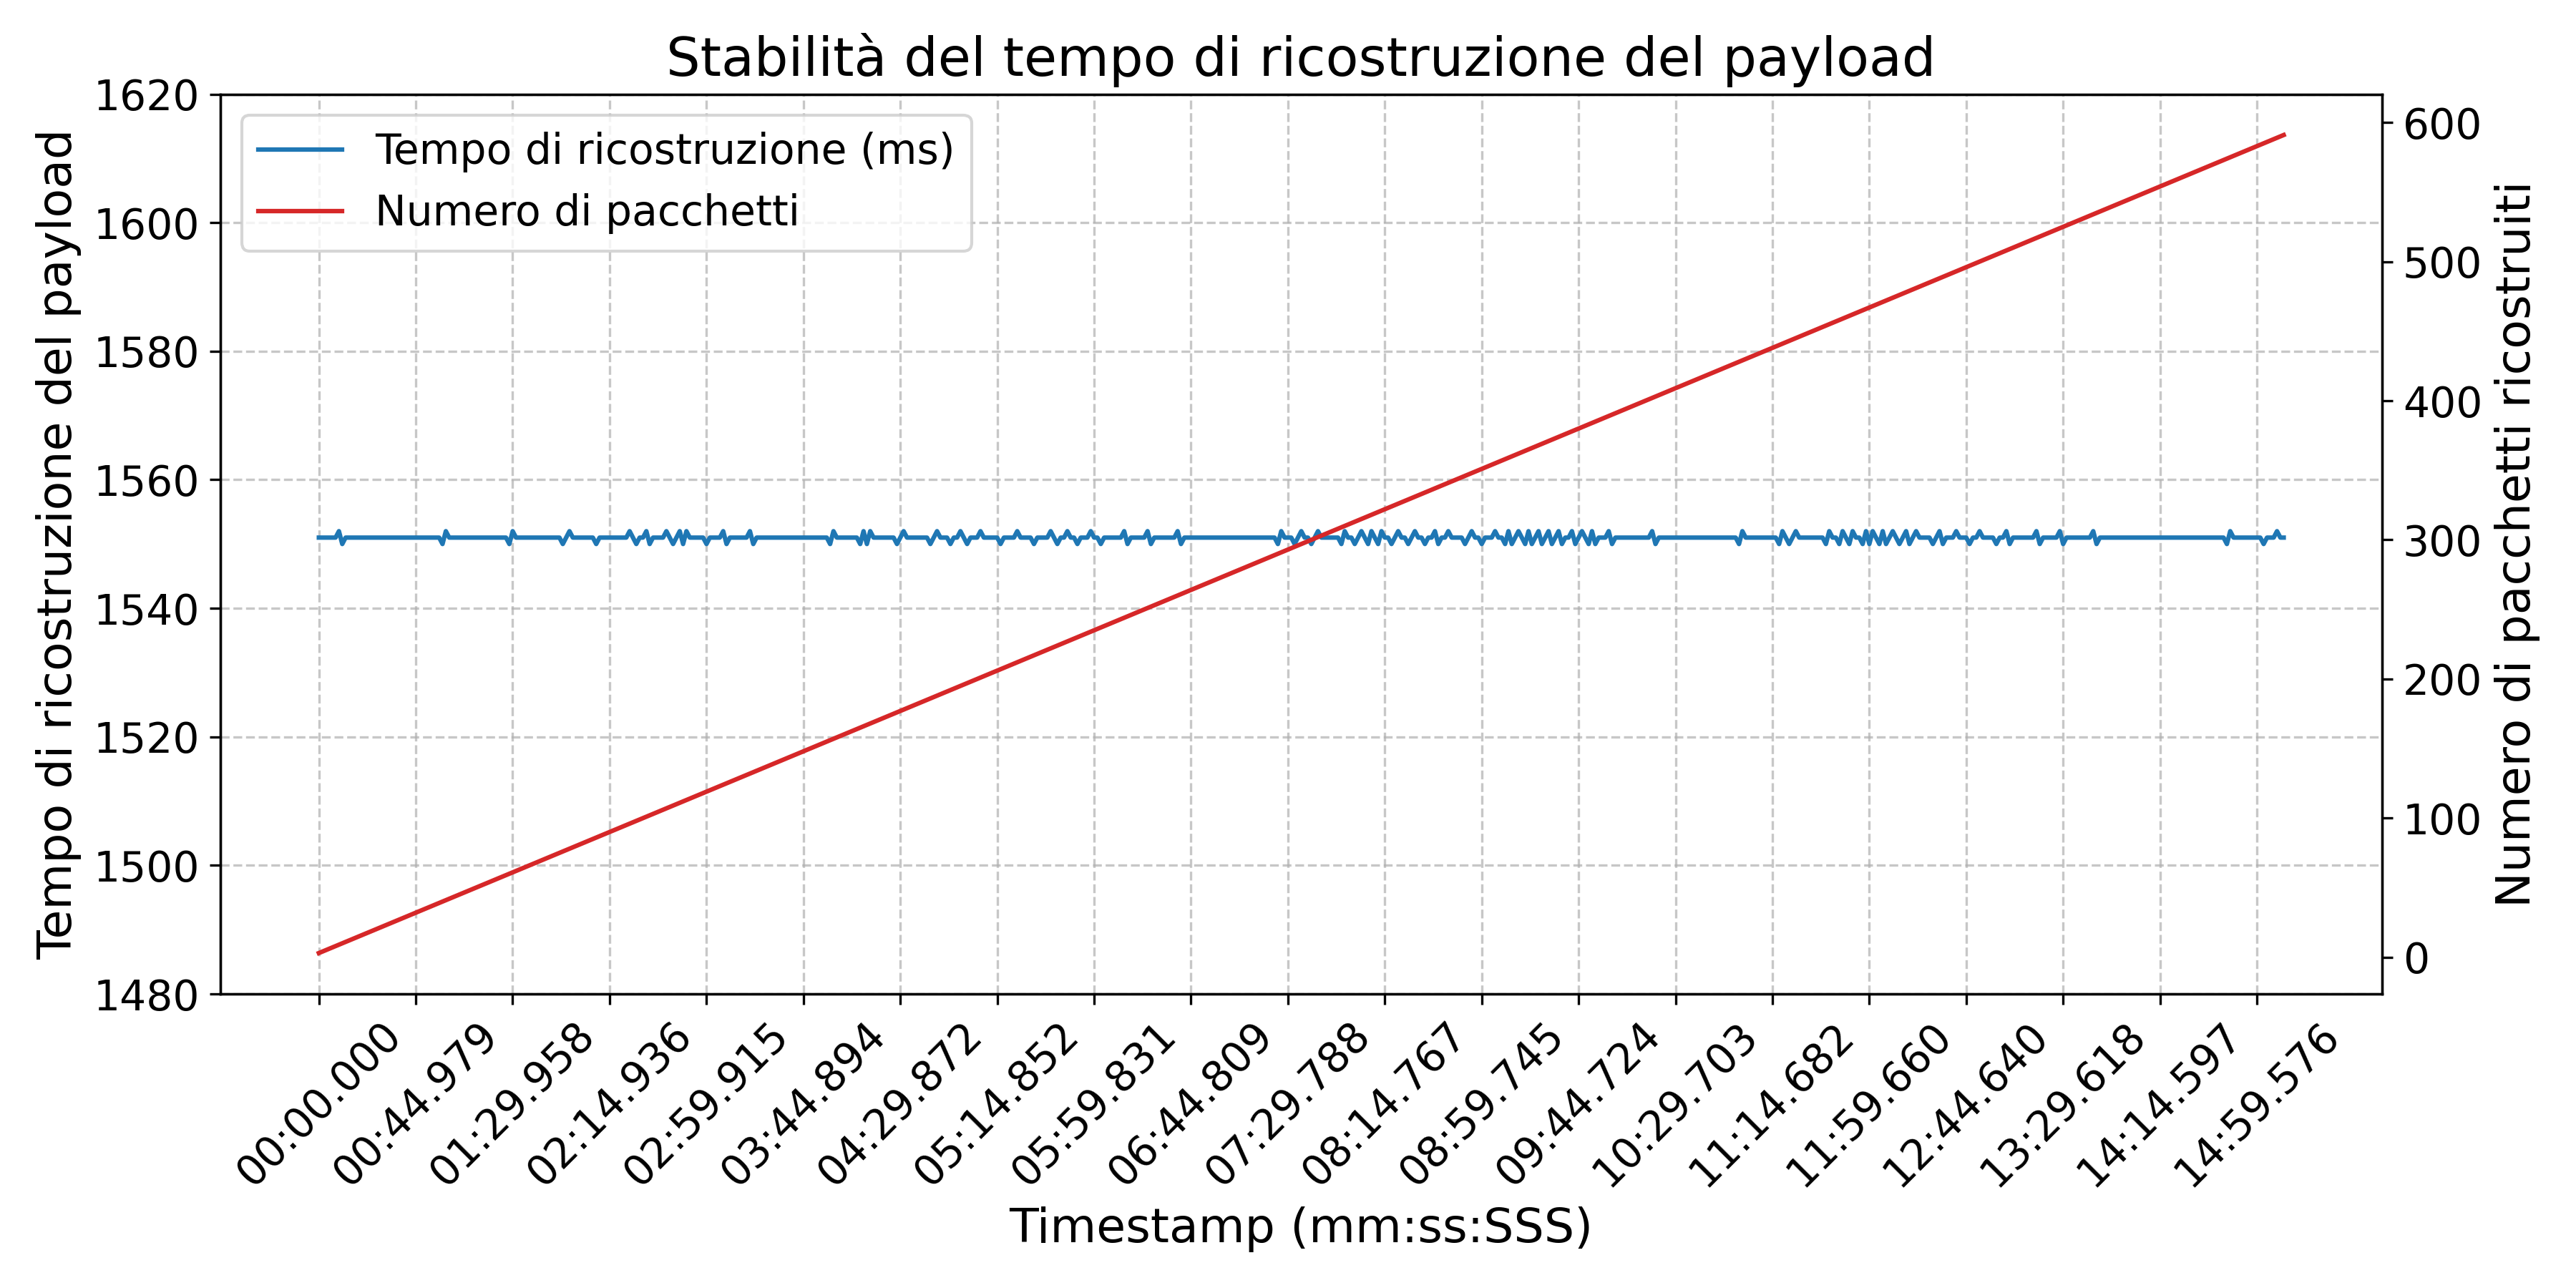
\includegraphics[width=\textwidth]{img/tests/T5/T5.png}
    \caption{Stabilità della comunicazione in assenza di interferenza diretta.}
    \label{fig:telemetry-robustness-test}
\end{figure}
\newpage

Anche nel secondo test, nonostante la presenza di una seconda antenna trasmittente
attiva sulla stessa frequenza, il sistema ha mantenuto una buona stabilità della
comunicazione, con un numero di pacchetti ricevuti in linea con le attese e senza
cali significativi di prestazioni, come mostrato nella figura~\ref{fig:telemetry-robustness-test-2}.

\begin{figure}[H]
    \centering
    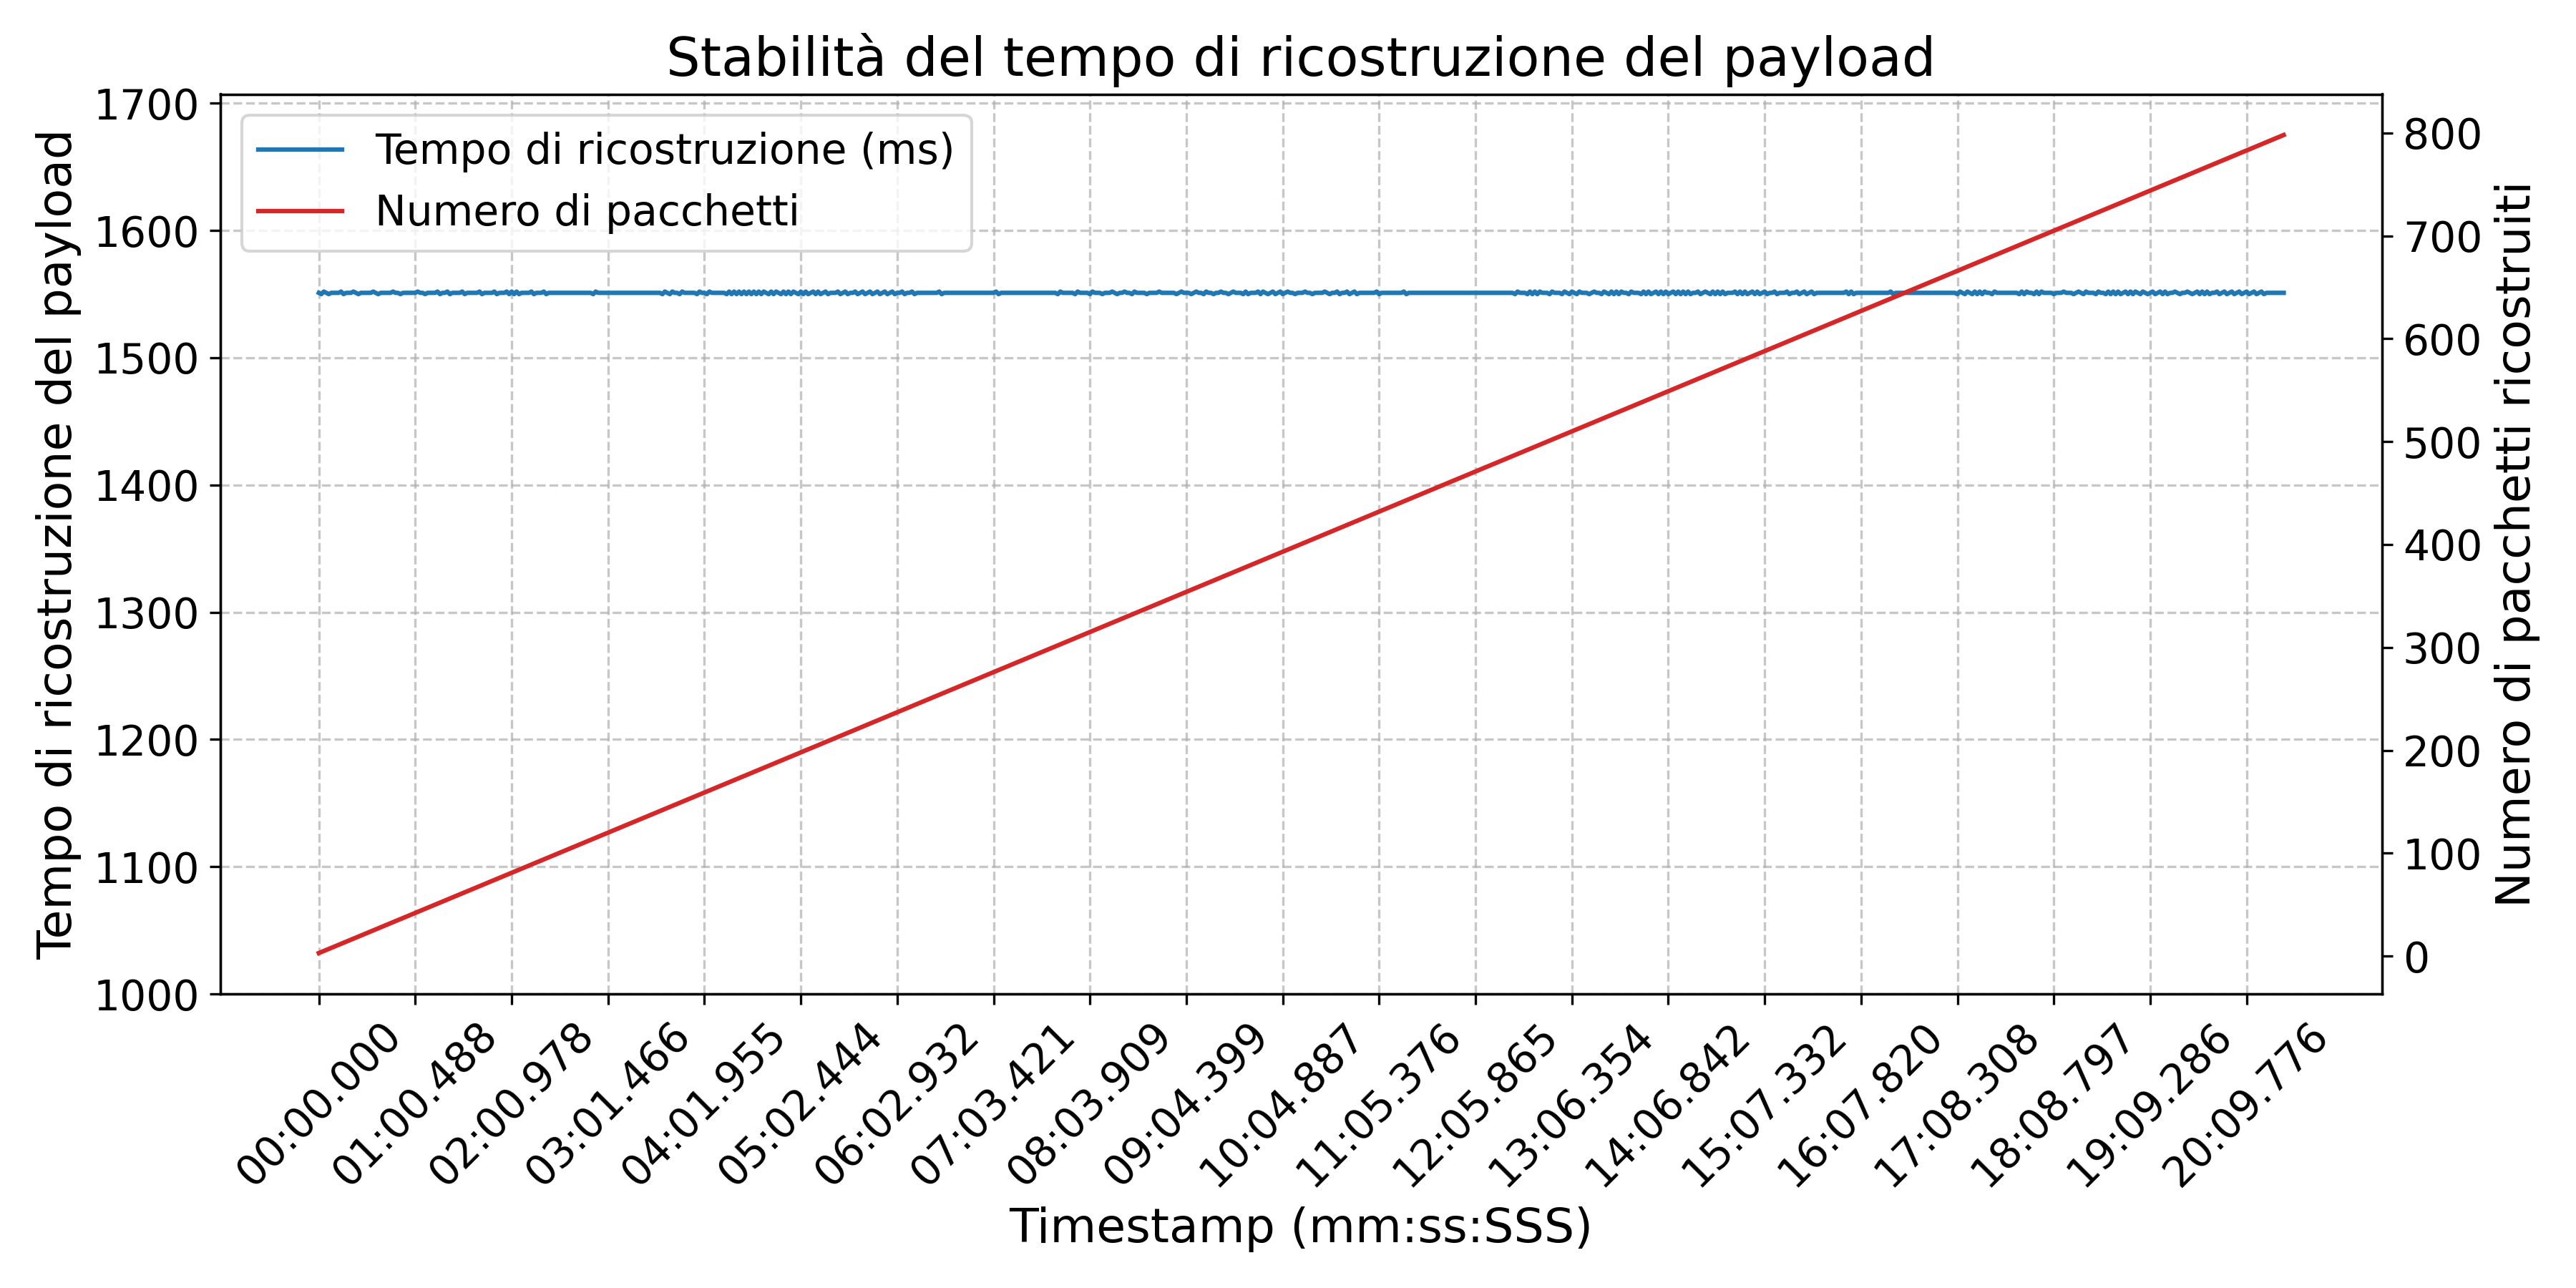
\includegraphics[width=\textwidth]{img/tests/T6/T6.png}
    \caption{Stabilità della comunicazione in presenza di interferenza diretta.}
    \label{fig:telemetry-robustness-test-2}
\end{figure}

Confrontando i risultati dei due test, si osserva che l'introduzione della seconda
antenna non ha avuto un impatto significativo sulla stabilità della comunicazione
né sulle prestazioni del sistema. Come illustrato nella figura~\ref{fig:telemetry-robustness-test-comparison},
i dati raccolti nei due scenari risultano sovrapponibili.

\begin{figure}[H]
    \centering
    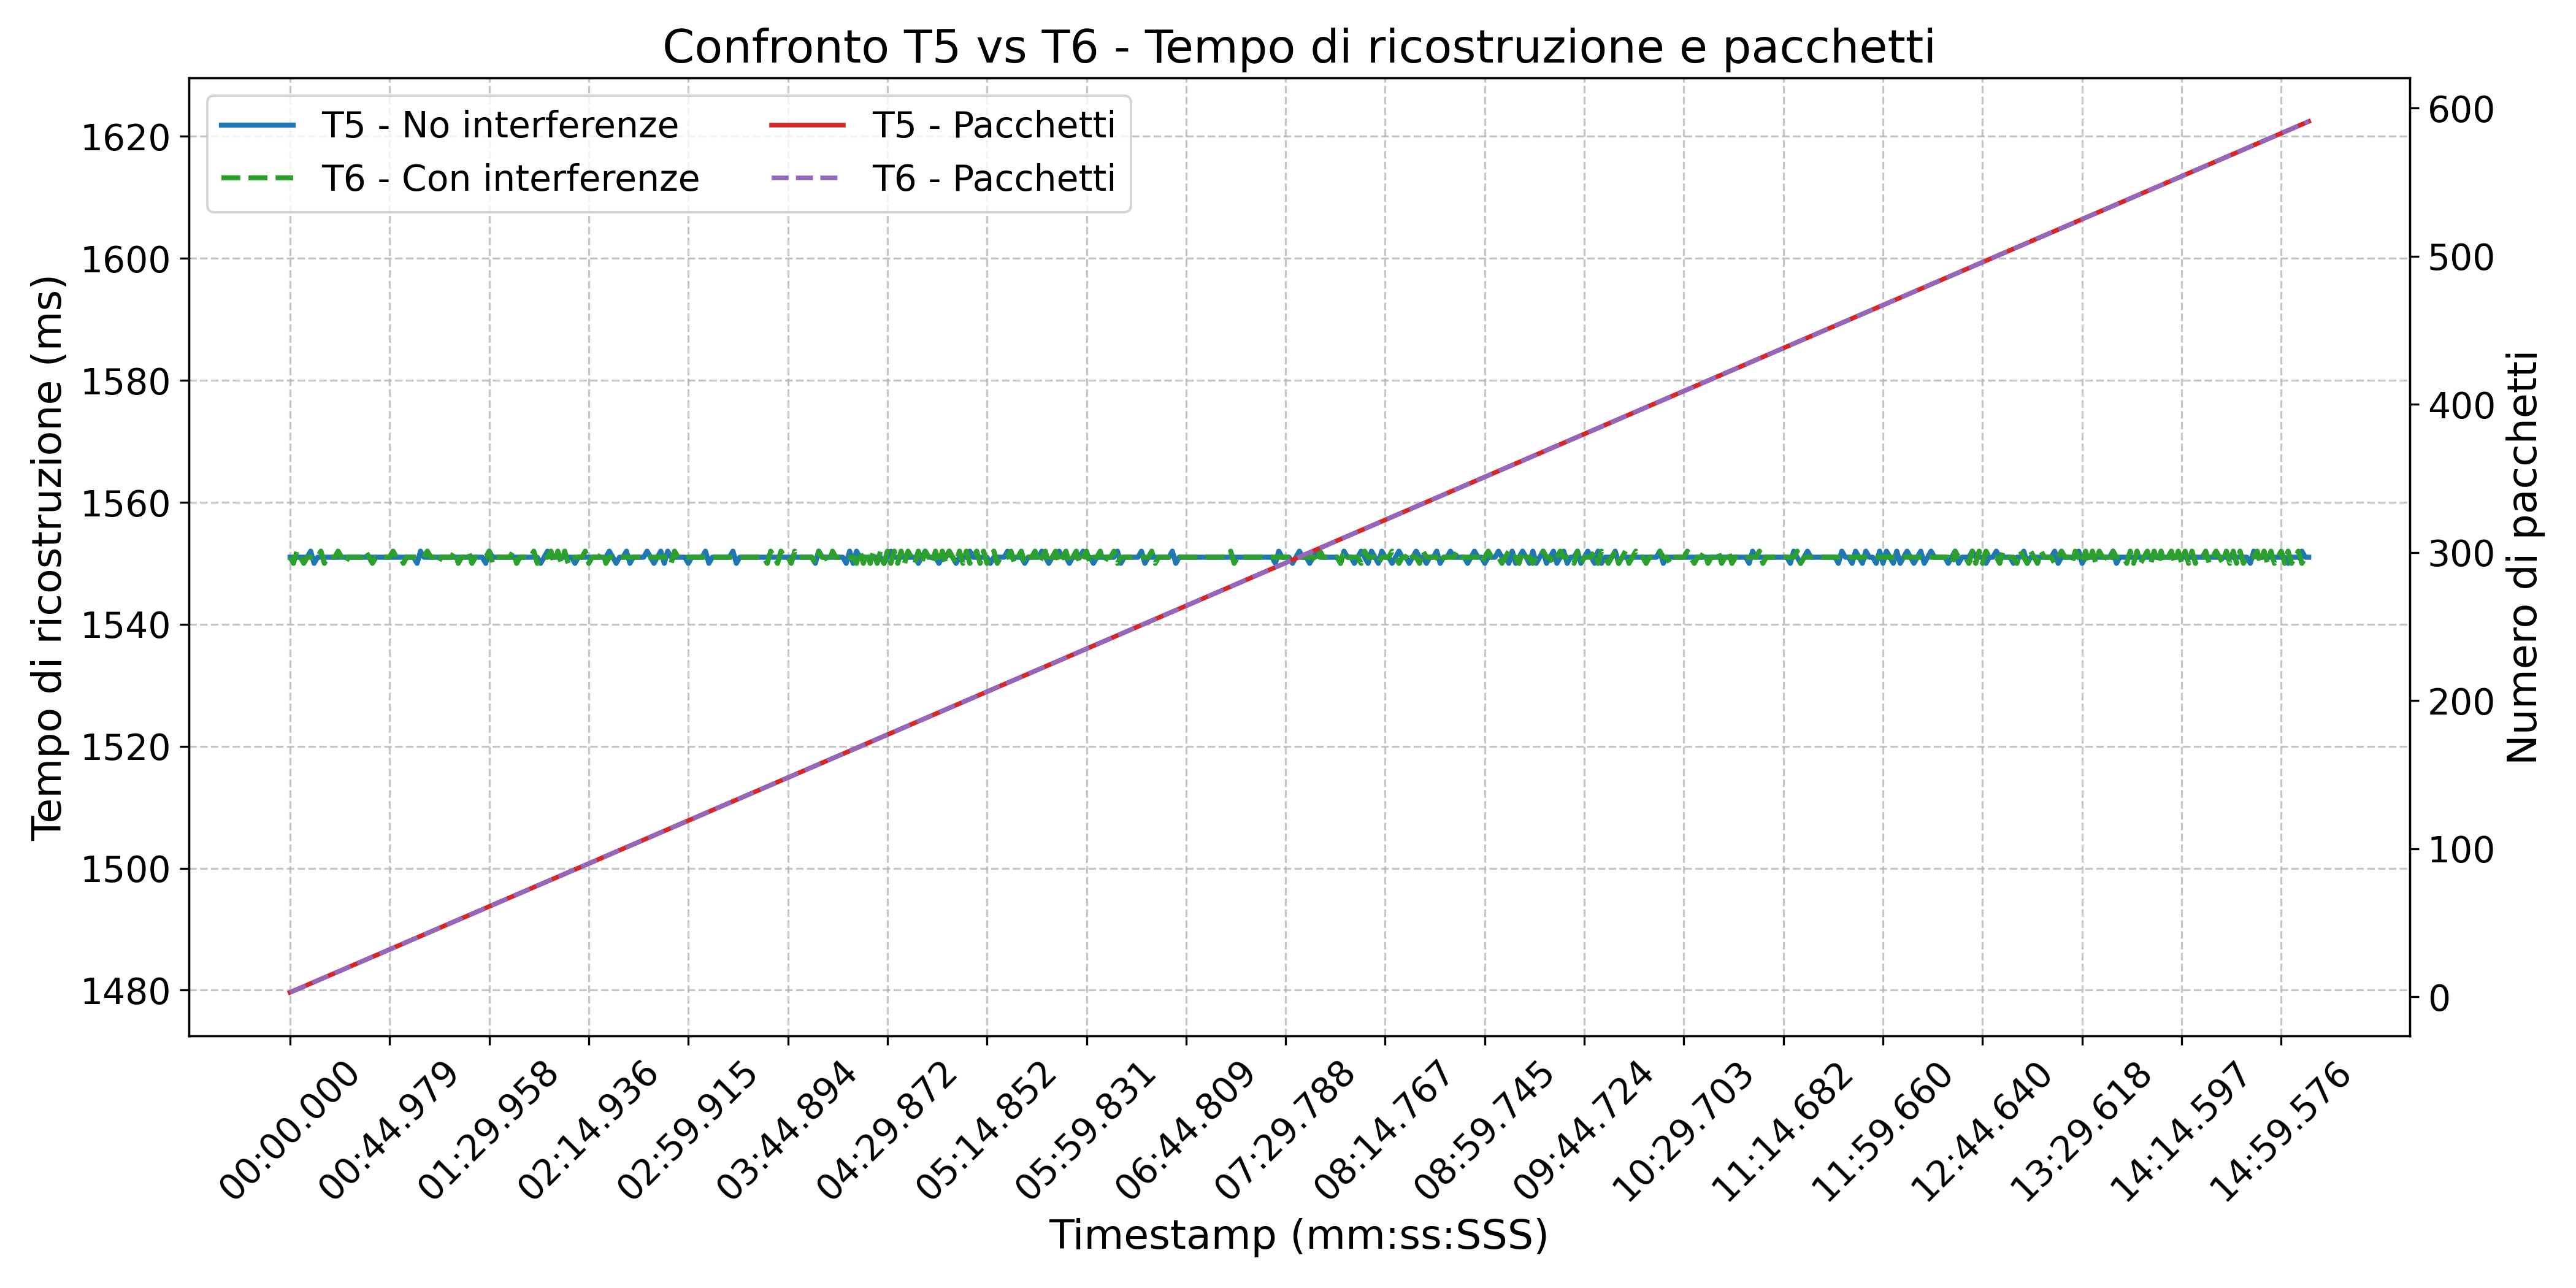
\includegraphics[width=\textwidth]{img/tests/T5-6/T5-6.png}
    \caption{Confronto tra i due test di robustezza.}
    \label{fig:telemetry-robustness-test-comparison}
\end{figure}

L'analisi numerica conferma che le differenze tra i due test sono trascurabili,
sebbene rilevabili. Come riportato nella tabella~\ref{tab:robustness-test-comparison},
la deviazione standard e la varianza dei tempi di ricostruzione sono leggermente
superiori nel test con interferenze, indicando una maggiore variabilità della
latenza di ricostruzione del \emph{payload}, imputabile alla presenza di
trasmissioni concorrenti.
\begin{table}[H]
    \centering
    \begin{tabular}{|l|c|c|}
        \hline
        \textbf{Metrica}                            & \textbf{Senza interferenze} & \textbf{Con interferenze} \\
        \hline
        Tempo di ricostruzione medio ($\delta_{r}$) & 1550.99                     & 1550.99                   \\ \hline
        Deviazione standard $\delta_{r}$            & 0.49                        & 0.62                      \\ \hline
        Varianza $\delta_{r}$                       & 0.24                        & 0.38                      \\ \hline
        Numero di pacchetti ricevuti                & 588                         & 588                       \\ \hline
        Numero di misure                            & 589                         & 589                       \\
        \hline
    \end{tabular}
    \caption{Confronto delle metriche statistiche tra test senza interferenze e con interferenze}

    \label{tab:robustness-test-comparison}
\end{table}

\newpage

\section{Limiti e possibili miglioramenti futuri}
Il sistema di telemetria sviluppato ha dimostrato buone prestazioni e un'elevata
affidabilità, ma presenta alcuni limiti che potrebbero essere oggetto di
miglioramento in sviluppi futuri.

Tra le criticità principali si segnala la necessità di ottimizzare la gestione
della latenza nella ricostruzione dei \emph{payload} segmentati, nonché il basso
\emph{throughput} dei moduli \ac{LoRa} impiegati, che limita la quantità di dati
trasmissibili nell’unità di tempo. Tali vincoli derivano dalle caratteristiche
intrinseche del protocollo LoRa e dall’architettura a pacchetti frammentati adottata.

Un ulteriore limite significativo riguarda la difficoltà di testare il sistema
in condizioni operative reali: il lancio di razzi sperimentali comporta infatti
complesse problematiche di natura legale, logistica, organizzativa ed economica,
che rendono difficile la pianificazione e l’esecuzione di prove realistiche in volo.

\section{Implicazioni del sistema sviluppato per progetti simili}
Il sistema di telemetria sviluppato per il progetto \emph{Borealis} rappresenta
una soluzione economica, affidabile e facilmente replicabile, potenzialmente
applicabile a un'ampia varietà di scenari nel campo della ricerca e dello sviluppo
di razzi sperimentali, ma non solo.

La modularità dell'architettura e l’impiego di tecnologie open-source consentono
una facile personalizzazione e integrazione con altri sottosistemi, rendendo il
progetto un solido punto di partenza per ulteriori sviluppi o adattamenti.

Il protocollo di comunicazione implementato, basato su segmentazione e
ricostruzione di \emph{payload}, estende le capacità di trasmissione offerte dai
moduli \ac{LoRa}, rendendolo adatto anche ad applicazioni che richiedono l’invio
affidabile di pacchetti di dati di medie dimensioni, pur operando in ambienti a
banda stretta e bassa latenza.

\chapter{Conclusioni} \label{chap:conclusion}
\section{Riepilogo dei risultati ottenuti}

Il progetto di telemetria sviluppato per il razzo \emph{Borealis} ha raggiunto
tutti gli obiettivi operativi prefissati.
I test sperimentali condotti hanno confermato la solidità del sistema in termini
di affidabilità, stabilità e resilienza operativa, evidenziando una copertura
adeguata, una gestione efficace della segmentazione dei dati e una comunicazione
stabile anche in condizioni avverse, quali disallineamento angolare tra le antenne
e presenza di interferenze co-canalari.

Il sistema ha dimostrato di essere tecnicamente valido, adattabile e compatibile
con i vincoli imposti da contesti aerospaziali a basso budget, confermando la bontà
delle scelte progettuali sia hardware che software.

\section{Riflessioni sull'impatto del progetto nell'ambito della ricerca e dello sviluppo di razzi sperimentali}
In letteratura sono documentati pochi progetti di telemetria per razzi sperimentali
basati su tecnologia \ac{LoRa}, la maggior parte dei quali si trova ancora a
livello di \emph{proof-of-concept} \cite{Andrade2022}, oppure non risulta adeguata
alle esigenze operative reali.
Ad esempio, il sistema presentato in \cite{Misbahuddin2022}, pur completo dal punto
di vista funzionale, si è dimostrato sottodimensionato sul piano prestazionale,
con un raggio operativo limitato a meno di 500 metri, un valore non compatibile con
scenari di volo suborbitale o a lungo raggio.

Altri lavori più recenti, come \cite{Brzynska2023,inproceedings}, mostrano dati sperimentali
promettenti, ma non approfondiscono lo sviluppo di protocolli di comunicazione
né la gestione strutturata dei dati come affrontato nel presente progetto.

A confronto con altri approcci documentati in letteratura, basati su tecnologie
differenti come WiFi \cite{muchiri2024implementation}, XBee \cite{10150/626955} con trasmettitori radio
ad alta potenza \cite{lombardozzo2017development,10150/666950}, il sistema
sviluppato per \emph{Borealis} offre un equilibrio ottimale tra portata, consumo
energetico e semplicità di implementazione.

L’uso efficiente dei moduli \ac{LoRa}, abbinato a un protocollo
personalizzato di segmentazione e ricostruzione, consente di ottenere distanze
operative di diversi chilometri con requisiti hardware minimi e consumi contenuti,
rendendo il sistema preferibile in molte applicazioni embedded in ambito aerospaziale
sperimentale.

In questo contesto, il sistema sviluppato per il progetto \emph{Borealis} si
distingue per l’approccio metodico, la modularità dell’architettura e la scalabilità,
oltre che per l’implementazione di un protocollo di comunicazione flessibile,
progettato per estendere in modo efficiente le capacità dei moduli \ac{LoRa}
anche in condizioni operative critiche.
Queste caratteristiche rendono il sistema adattabile e riutilizzabile in una
varietà di contesti, contribuendo in modo significativo all’avanzamento dello stato
dell’arte nei sistemi di telemetria embedded a basso consumo.

\section{Prospettive di sviluppo futuro}
\subsection{Miglioramenti al sistema di telemetria}
\subsubsection{Utilizzo di antenne \emph{patch}}
L'utilizzo di un'antenna elicoidale omnidirezionale si \'e rivelato efficace, tuttavia,
per migliorare la copertura e la direzionalit\'a, e per ridurre le dimensioni del sistema,
si potrebbe considerare l'uso di antenne \emph{patch}, da applicare sulla fusoliera del razzo,
in questo modo si elimina il problema del mascheramento del segnale dovuto al materiale della fusoliera
(alluminio o fibra di carbonio), eliminando la necessità di inserire la finestra in plexiglass utilizzata
su Borealis. In questo modo migliorerebbero anche le propriet\'a strutturali e aerodinamiche del razzo.
\subsubsection{Utilizzo di moduli \ac{LoRa} con maggiore \emph{throughput}}
I moduli \ac{LoRa} EByte E220-900T22D utilizzati hanno dimostrato buone prestazioni
in termini di portata e affidabilità, ma presentano un limite di \emph{throughput} che
può essere migliorato utilizzando moduli con capacità di trasmissione dati più elevate.
Moduli come i moduli della serie Semtech SX126x offrono un \emph{throughput} maggiore e
una maggiore flessibilità nella configurazione dei parametri di trasmissione, a fronte
di un costo superiore e del minore support software rispetto ai moduli EByte.
\subsection{Miglioramenti al protocollo di comunicazione}
\subsubsection{Implementazione di un sistema di \emph{retransmission}}
Attualmente il protocollo di comunicazione implementato non prevede un meccanismo di \emph{retransmission} dei pacchetti persi,
si potrebeb valutare l'implementazione di un sistema di \emph{retransmission} da coadiuvare al meccanismo di \emph{drop} temporizzato dei pacchetti,
in modo da ridurre il numero di pacchetti persi in caso di errori di trasmissione o di congestione della rete.
Questo potrebbe essere realizzato implementando un sistema di \emph{acknowledgment} dei pacchetti,
tuttavia, bisogna valutare l'impatto che questo potrebbe avere sul \emph{throughput} del sistema.
\subsection{Parsing dei dati e visualizzazione}
\subsubsection{Implementazione di un sistema di visualizzazione in tempo reale}
\'E prevista l'implementazione di una \emph{dashboard}, per poter monitorare il
volo del razzo in tempo reale.
Si prevede di utilizzare un sistema di visualizzazione basato su \emph{Flask},
che permetterebbe di visualizzare i dati raccolti in tempo reale tramite un'interfaccia web.

\newpage
\renewcommand{\appendixtocname}{Appendici}
\renewcommand{\appendixpagename}{Appendici}
% \csname @openrightfalse\endcsname
\pagenumbering{gobble}
\begin{appendices}
    % \library{url}{name}{description}{label}
    % or
    % \library[url=...,name=...,description=...,label=...]
    % 
    % This command creates a hyperlink with a bold name and a description, 
    % and assigns a label for referencing.
    % 
    % Parameters:
    %   #1: The URL to link to.
    %   #2: The name to display in bold.
    %   #3: The description to display after the name.
    %   #4: The label for referencing.
    \newcommandx{\library}[4]{\item \href{#1}{\textbf{#2}} - #3\label{#4}}
    \renewcommand{\thechapter}{\Alph{chapter}} % Per avere "Appendice A, B, C..."
    \chapter{Librerie} \label{app:librerie}
    \begin{enumerate}
        \library{https://github.com/xreef/EByte_LoRa_E220_Series_Library}%
        {EByte LoRa E220 Series}%
        {Per la gestione dei moduli \ac{LoRa} E220.}{lib:lora}
        \library{https://github.com/adafruit/Adafruit_Sensor}%
        {Adafruit Unified Sensor}%
        {Per le API standard di gestione dei sensori.}{lib:uni-sensor}
        \library{https://github.com/adafruit/Adafruit_BNO055}%
        {Adafruit BNO055}%
        {Per la gestione della \ac{IMU}.}{lib:bno055}
        \library{https://github.com/adafruit/Adafruit_MPRLS}%
        {Adafruit MPRLS}%
        {Per la gestione dei barometri MPRLS.}{lib:mprls}
        \library{https://github.com/greiman/SdFat}%
        {Adafruit SDFat}%
        {Per la gestione del logging su scheda SD.}{lib:sdfat}
        \library{https://github.com/nlohmann/json}%
        {nlohmann-json}%
        {Per la gestione di oggetti JSON in C++.}{lib:json}
    \end{enumerate}

    \chapter{Datasheet} \label{app:datasheet}
    \begin{enumerate}
        \library{https://www.cdebyte.com/pdf-down.aspx?id=3552}%
        {Datasheet EByte E220-900T22D}%
        {Datasheet del modulo EByte E220-900T22D.}{ds:lora}
        \library{https://www.mouser.it/datasheet/2/1161/Delta_5A_Datasheet_Rev_2_2-2486634.pdf}%
        {Datasheet Siretta Delta 5A}%
        {Datasheet dell'antenna omnidirezionale Siretta Delta 5A.}{ds:omni}
        \library{https://www.siretta.com/?sdm_process_download=1&download_id=3401}%
        {Datasheet Siretta Oscar 3A}%
        {Datasheet dell'antenna Yagi Siretta Oscar 3A.}{ds:yagi}
    \end{enumerate}

    \chapter{Dati di test} \label{app:test}
    \begin{enumerate}
        \library{https://docs.google.com/spreadsheets/d/18jeeM74zrUXYElvqgezdn9tdanWeXri5lLqX9B6a6Do/edit?usp=sharing}%
        {Disallineamento delle antenne}%
        {Dati raccolti durante i test di disallineamento delle antenne.}{test:misalignement}
        \library{https://docs.google.com/spreadsheets/d/1uNnyeW3Q8s5x24YAA0kJOUTOkH-Pz_z4T3AYBhDrex0/edit?usp=sharing}%
        {Test del \emph{throughput}}%
        {Dati raccolti durante i test di throughput del protocollo di comunicazione.}{test:throughput}
        \library{https://docs.google.com/spreadsheets/d/1S1JPVLed6u9Xg_fJpRhLmknomVhyZoRTk6BMkn2IwYY/edit?usp=sharing}%
        {Test di segmentazione e ricostruzione dei dati}%
        {Dati raccolti durante i test di segmentazione e ricostruzione dei dati.}{test:segmentation}
        \library{https://docs.google.com/spreadsheets/d/12eh43EHKv12Hg0LvEx2MS6zIxmNwMrx_Yy7wnoK4u0s/edit?usp=sharing}%
        {Test del meccanismo di \emph{drop}}%
        {Dati raccolti durante i test del meccanismo di \emph{drop} dei pacchetti.}{test:drop}
        \library{https://docs.google.com/spreadsheets/d/1GKSbkaEbUHr0ZOiz14gFqvqbBCe8doklDKrzemptGEw/edit?usp=sharing}%
        {Test di riordinamento dei pacchetti}%
        {Dati raccolti durante i test di riordinamento dei pacchetti.}{test:reordering}
        \library{https://docs.google.com/spreadsheets/d/1xAPwyOoEX-zgcn06yl7xqlSX9hobIEPWwbrz_aBrxHM/edit?usp=sharing}%
        {Test di robustezza e affidabilità}%
        {Dati raccolti durante i test di robustezza e affidabilità del protocollo di comunicazione.}{test:robustness}
    \end{enumerate}
    % \chapter{Embed di interi PDF}
    % \label{Appendice:C}
    % Se ti serve puoi fare embed di PDF interi con pdfpage, scegliendo anche le pagine (o mettendo - se le vuoi tutte):

    % 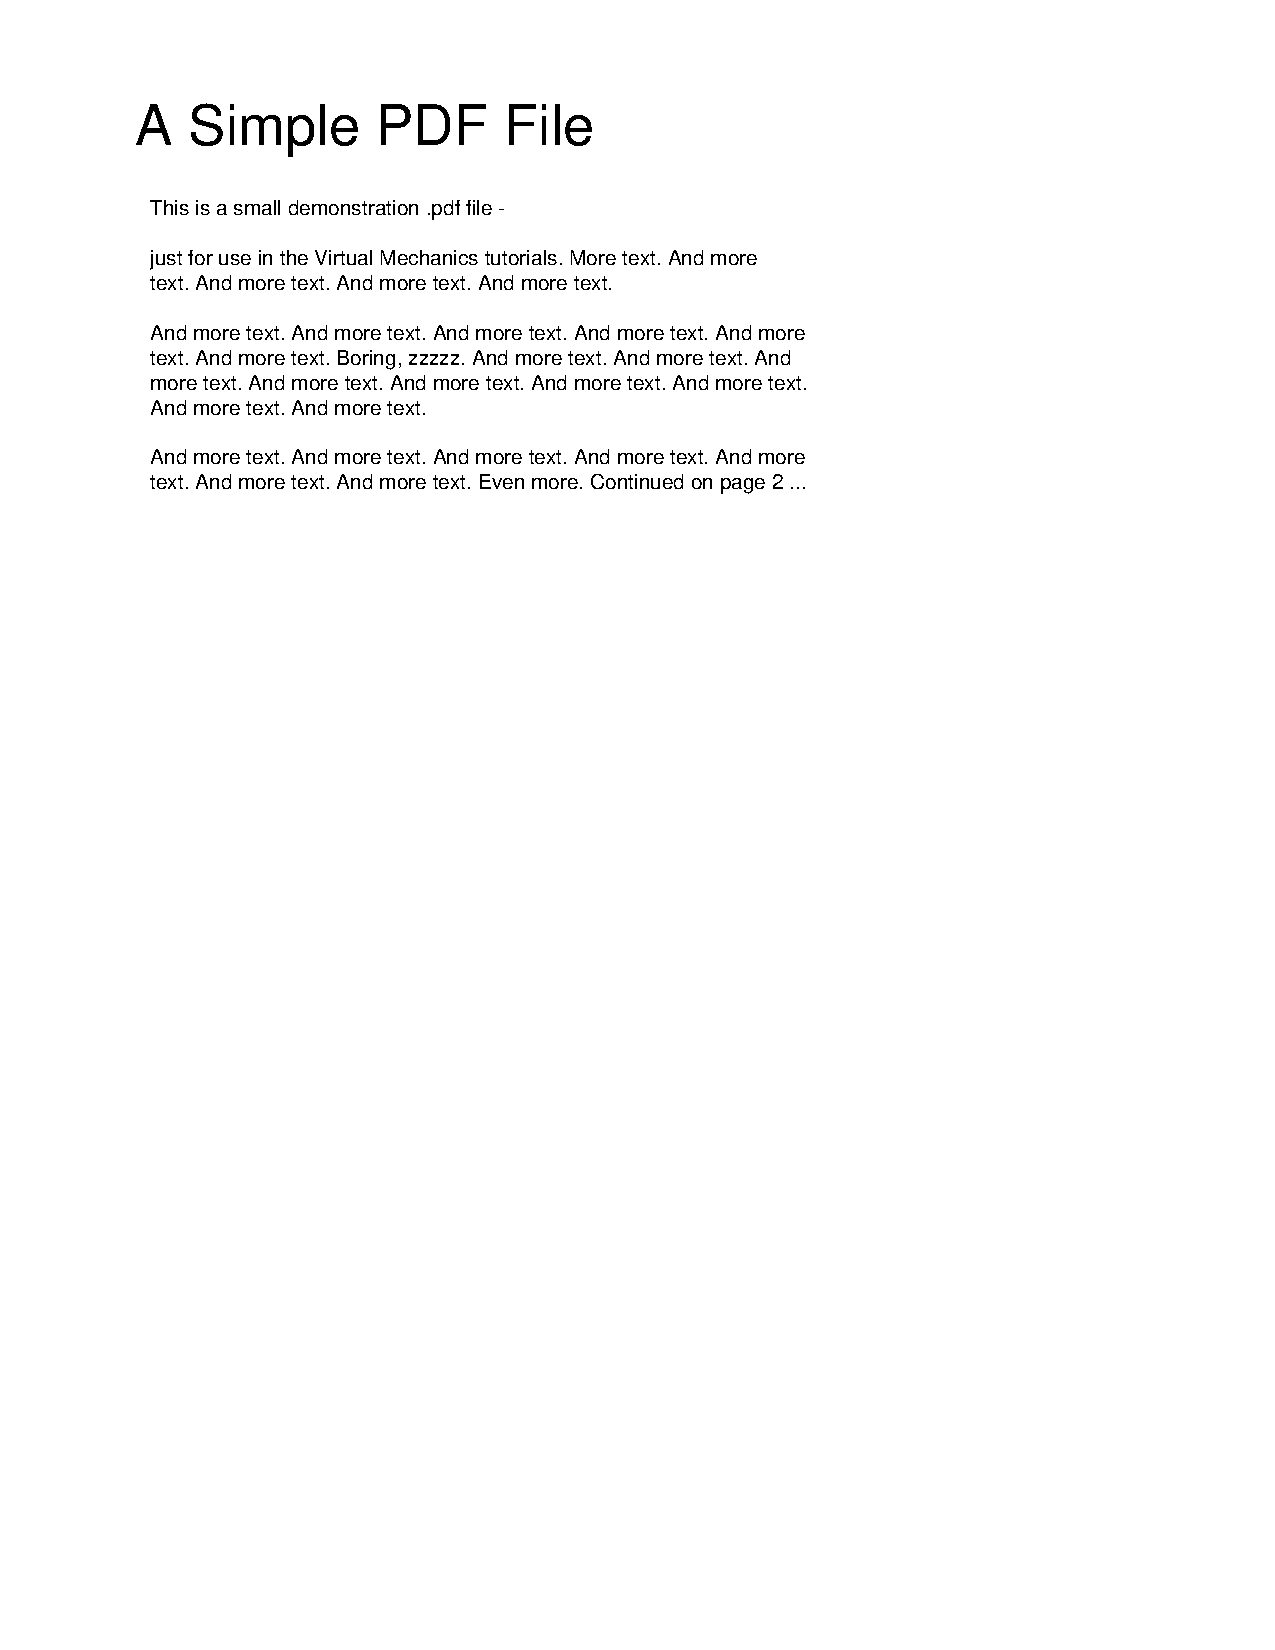
\includepdf[pages=1]{pdf/sample.pdf}
\end{appendices}
% \section{elenchi}
% \subsection{Elenchi puntati}
% \begin{itemize}
%     \item bla
%     \begin{itemize}
%         \item sub-bla
%     \end{itemize}
%     \item bla
% \end{itemize}

% \subsection{Elenchi numerati}
% \begin{enumerate}
%     \item bla1
%     \begin{enumerate}
%         \item sub bla 1
%         \item sub bla 2
%     \end{enumerate}
%     \item bla 2
% \end{enumerate}

% \subsection{Mix}
% \begin{itemize}
%     \item bla
%     \begin{enumerate}
%         \item sub bla 1
%     \end{enumerate}
%     \item bla
% \end{itemize}

% \begin{enumerate}
%     \item bla 1
%     \begin{itemize}
%         \item sub bla
%     \end{itemize}
%     \item bla 2
% \end{enumerate}

% \section{Font}
% \textbf{bla bla bla}\\
% \textit{Ancora bla bla bla}\\
% \texttt{bla bla ma in un'altra riga}

% \subsection{Sottosezione 1 - parskip}
% Grazie al package parskip se vai a capo nel .tex lasciando una riga

% ti mette un po' di spazio anche nel pdf.\\
% Attenzione però che ogni tanto questa feature fa lasciare troppo spazio tra testo e immagini / tabelle, se capita prova a togliere un po' di righe vuote. \\
% Senza questo pacchetto, una doppia new line (\texttt{$\backslash n\backslash n$}) crea un nuovo paragrafo, la cui prima riga viene leggermente indentata (un comportamento indesiderato se vieni da altri strumenti di stesura). Eventualmente, si può usare per allungare di qualche pagina alla tesi, evitando di abusarne.
% \subsection{Sottosezione 2 - capitoli}
% I capitoli iniziano sempre in una pagina dispari, quindi a volte vedrai delle pagine bianche tra uno e l'altro
% \subsubsection{Sottosottosezione 1} \label{subsub:bla}
% bla bla bla

% \chapter{Dopo l'introduzione}
% qua scrivi qualcosa
% \section{Immagini}
% Quando fai begin figure, ricordati di mettere tra quadre un modificatore di posizione: H significa esattamente nel punto dove si trova l'immagine nel file .tex e ti consiglio di usare quello, se no ci sono ad esempio t (top) e b (bottom).

% \begin{figure}[H]
%     \centering
%     % Se metti solo una delle due dimensioni, l'altra scala in automatico
%     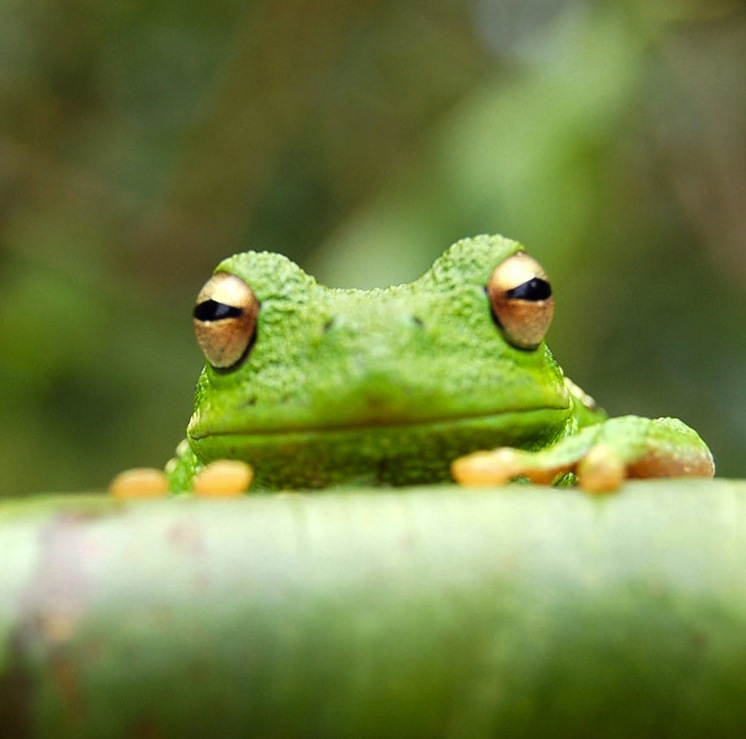
\includegraphics[height = 6cm, width=8cm]{img/frog.jpg}
%     \caption{Caption (questo viene scritto nell'indice delle figure)}
%     % La label ci vuole sempre e te la inventi tu: serve per riferirsi alle immagini successivamente
%     \label{fig:frog}
% \end{figure}

% \section{tabelle}
% \subsection{Tabella semplice}
% Anche qui nota H tra quadre, la caption e la label

% \begin{table}[H]
%     \centering
%     \begin{tabular}{|c|c|}
%     \hline
%         \textbf{Pratiche agili} & \textbf{Studenti}  \\ \hline
%         Sprint planning & 73  \\ \hline
%         Pair programming & 73  \\ \hline
%         Retrospettiva & 48  \\ \hline
%     \end{tabular}
%     \caption{Tabella semplice (anche questo scritto nell'indice delle tabelle)}
%     \label{tab:simple}
% \end{table}

% \subsection{tabelle avanzate}
% Con multirow (e multicolumn che però serve meno) puoi fare righe (colonne) più grandi del normale.\\
% \begin{table}[H]
%     \centering
%     \begin{tabular}{|c|c|c|c|c|}
%     \hline
%         \textbf{Team} & \textbf{LoC verificate} & \textbf{LoC sviluppatori} & \textbf{Ore sviluppatori} & \textbf{LoC/h}  \\ \hline
%         \multirow{2}*{1} & 1148& m: 888& m: 40& 22\cr & Diff: -1852& $\sigma$: 371& $\sigma$: 27& \\ \hline
%         \multirow{2}*{2}&1858& m: 1404& m: 65& 22\cr &  Diff: -448& $\sigma$: 1222& $\sigma$: 78& \\ \hline
%         \multirow{2}*{3}&1640& m: 1400& m: 96& 15\cr &  Diff: -2810& $\sigma$: 1417& $\sigma$: 41& \\ \hline
%     \end{tabular}
%     \caption{CAPTION}
%     \label{tab:avanz}
% \end{table}

% \subsubsection{Tabelle girate}
% Se usi landscape la tabella viene girata (nel caso dovessi inserirne una molto grande)
% \begin{landscape}
% \begin{table}[H]
%     \centering
%     \begin{tabular}{|c|c|}
%     \hline
%         \textbf{Numero} & \textbf{\#}  \\ \hline
%         UNO & 1  \\ \hline
%         DUE & 2  \\ \hline
%         TRE & 3  \\ \hline
%     \end{tabular}
%     \caption{Tabella girata}
%     \label{tab:girata}
% \end{table}

% \end{landscape}

% \section{Grafici}
% Puoi creare grafici con tikzpicture.
% Qui c'e' un grafico con asse x e y customizzabili per ogni tipo d'utilizzo.
% Tutti i tool e tutorial necessari per creare ogni tipo di grafico puo' essere trovato qui: https://tikz.dev/

% \begin{tikzpicture}
%   % Draw x-axis
%   \draw[->] (-1,0) -- (15,0) node[right] {$x$};
%   % Draw y-axis
%   \draw[->] (0,-1) -- (0,5) node[above] {$y$};

%   % Draw grid lines (optional)
%   \foreach \x in {1,2,3,4,5,6,7,8,9,10,11,12,13,14}
%     \draw (\x,-0.1) -- (\x,0.1);
%   \foreach \y in {1,2,3,4}
%     \draw (-0.1,\y) -- (0.1,\y);

%   % Draw origin
%   \fill (0,0) circle[radius=2pt];
% \end{tikzpicture}

% \section{Import di file TeX}
% Puoi importare altri file tex per intero includendoli cosi'.
% Questo e' molto utile per mettere insieme diversi capitoli di una tesi o di un grande documento in generale.

% Questo e' il contenuto del documento imported\textunderscore document.tex


% \chapter{Altri comandi}
% bla bla
% \section{Math mode}
% Per inserire simboli matematici (e lettere greche) serve la math mode:

% Usando il simbolo del dollaro hai la math mode inline: $5 \times \alpha = 3\lambda$

% Altrimenti hai quella con le barre e le quadre \[ \frac{\sum_6^i 3i\theta}{12k^2\times 7}\]

% Infine hai quelle con begin equation (che vengono numerate):
% \begin{equation}
%     \frac{1}{2}\times A_{bcd}\times E^{fgh}
% \end{equation}

% Anche le equazioni possono avere label.
% \section{url e footnote}
% per mettere un link usa url: \url{wikipedia.it}

% per fare note a piè di pagina usa footnote\footnote{Tipo questa}

% \section{Code snippets}
% per inserire code snippets, puoi usare lstlisting

% \begin{lstlisting}[language=c]
% #include<stdio.h>

% int main(void) {
%     printf("Hello World\n");
%     return 0;
% }
% \end{lstlisting}

% \section{verbatim}
% Se ti serve scrivere codice o qualcosa per cui ti serve una formattazione specifica usa verbatim:
% \begin{verbatim}
%     Qui puoi scrivere

%     come      vuoi
%     e viene tutto

% scritto
%                     monospaziato
% \end{verbatim}
%\section{riferimenti}
% Come detto prima le label servono per riferirsi ad altre parti del testo citate precendentemente.\\
% Ti consiglio di metterle sempre almeno a figure. immagini e capitoli.

% Per riferirti a qualcosa basta fare ref seguito dal nome della label, ad esempio ``vedi capitolo \ref{chap:intro}''.\\In questo modo dal pdf cliccando sulla reference, ti porta direttamente al punto giusto.
% Altri pacchetti come \texttt{fancyref} e \texttt{cleveref} (consigliato) possono aiutare nell'automatizzare la creazione delle refrence. Usando ad esempio \texttt{\cref{chap:intro}} viene generata la dicitura corrispondete all'elemento a cui si fa riferimento, seguita dalla numerazione. Eccone un esempio: \cref{chap:intro}.
%\section{citazioni}
% Per citare si usa cite seguito dal nome dell'articolo nel file.bib, ad esempio ``come visto nell'articolo di tizio\cite{greenwade93}''.

% Se non ti piace lo stile di citazione puoi modificarlo sopra dove scrivo usepackage natbib, ma quello impostato attualmente dovrebbe andare bene.



\renewcommand{\bibsection}{}
\chapter*{Riferimenti bibliografici}
\bibliography{refs}
\newpage

\newpage~\newpage
\chapter*{Ringraziamenti}
Grazie a tutti!
\end{document}
